\documentclass[12pt,a4paper]{article}

% ==================== FONT / ENCODING ====================
\usepackage[utf8]{inputenc}
\usepackage[T5]{fontenc}
\usepackage{mathptmx}

% ==================== TOÁN HỌC ====================
\usepackage{amsmath,amssymb,amsfonts,yhmath}
\numberwithin{figure}{subsection}

% ==================== LAYOUT ====================
\usepackage[top=2cm, bottom=2cm, left=3cm, right=2cm]{geometry}
\usepackage{setspace}
\onehalfspacing

\usepackage{indentfirst}
\setlength{\parindent}{1.1cm}

% ==================== DANH SÁCH / BẢNG / HÌNH ====================
\usepackage{enumitem}
\usepackage[table]{xcolor}
\usepackage{booktabs}
\usepackage{array}
\usepackage{graphicx}
\usepackage{float}

% ==================== TIKZ ====================
\usepackage{tikz}
\usetikzlibrary{
    calc,
    arrows.meta,
    shadows,
    decorations.pathreplacing
}

% ==================== MÀU SẮC ====================
\definecolor{uehred}{RGB}{210, 50, 40}
\definecolor{uehteal}{HTML}{2D5D66}
\definecolor{uehorange}{HTML}{D96B42}
\definecolor{uehblue}{HTML}{1A408B}
\definecolor{vscodebg}{HTML}{1E1E1E}
\definecolor{vscodegreen}{HTML}{6A9955}
\definecolor{vscodetext}{HTML}{D4D4D4}
\definecolor{LightGray}{gray}{0.9}


\definecolor{genBlue}{RGB}{230, 240, 255}
\definecolor{genGreen}{RGB}{230, 255, 230}
\definecolor{genOrange}{RGB}{255, 240, 230}
\definecolor{lineBlue}{RGB}{60, 120, 200}
\definecolor{lineGreen}{RGB}{60, 160, 80}
\definecolor{lineOrange}{RGB}{210, 120, 50}

% ==================== TITLE / SECTION ====================
\usepackage{titlesec}
\titleformat{\section}{\Large\bfseries}{\thesection}{1em}{}
\titleformat{\subsection}{\large\bfseries}{\thesubsection}{1em}{}

% ==================== CÁC GÓI KHÁC CỦA FILE GỐC ====================
\usepackage{fontawesome5}
\usepackage[solcolor]{ex_test}
\usepackage{anyfontsize}
\usepackage{longtable}
\usepackage{makecell}
\usepackage{pdflscape}

\hypersetup{unicode}
\graphicspath{{resources/}}

% ==================== MINTED: CODE PYTHON TỰ XUỐNG DÒNG ====================

\usepackage{minted}
\setminted{
    frame=lines,
    framesep=2mm,
    baselinestretch=1.1,
    bgcolor=lightgray!15,
    fontsize=\small,
    linenos,
    breaklines=true,
    breakanywhere=true,
    autogobble=true
}

\renewcommand{\theFancyVerbLine}{
    \textcolor{gray!60!white}{\scriptsize\arabic{FancyVerbLine}}
}

% ==================== ALGORITHM: DÙNG BẢN BREAKABLE ====================
% Không dùng \begin{algorithm}[H] cho thuật toán dài nữa,
% vì algorithm là float và dễ bị nhảy nguyên khối sang trang sau.
\usepackage{algpseudocode}
\usepackage{caption}
\usepackage[most]{tcolorbox}
\tcbuselibrary{breakable}
\usepackage{tabularx}      % Bắt buộc cho môi trường tabularx và cột X

\newcounter{breakablealgocounter}

\newenvironment{breakablealgorithm}[1]
{
    \refstepcounter{breakablealgocounter}
    \begin{tcolorbox}[
        breakable,
        enhanced,
        colback=white,
        colframe=black!55,
        sharp corners,
        boxrule=0.5pt,
        left=2mm,
        right=2mm,
        top=1mm,
        bottom=1mm,
        title={Algorithm \thebreakablealgocounter. #1},
        fonttitle=\bfseries
    ]
}
{
    \end{tcolorbox}
}

% ==================== VIỆT HÓA ====================
\renewcommand{\contentsname}{Mục lục}
\renewcommand{\figurename}{Hình}
\renewcommand{\tablename}{Bảng}
\renewcommand{\refname}{Tài liệu tham khảo}

% ==================== CUSTOM TOÁN HỌC ====================
\renewcommand{\ge}{\geqslant}
\renewcommand{\geq}{\geqslant}
\renewcommand{\le}{\leqslant}
\renewcommand{\leq}{\leqslant}

\newcommand{\tron}[1]{\left( #1 \right)}
\newcommand{\vuong}[1]{\left[ #1 \right]}
\newcommand{\nhon}[1]{\left\{ #1 \right\}}
\newcommand{\sieuto}[1]{\Big( #1 \Big)}

\begin{document}

% ==================== TRANG BÌA ====================
\begin{titlepage}

\begin{tikzpicture}[remember picture, overlay]
    \node[inner sep=0pt] at (current page.center) {
        
\includegraphics[width=1.1\paperwidth, height=1\paperheight]{resources/khung_pdf.pdf}
    };
\end{tikzpicture}

\centering
\vspace*{0.2cm}

{\small BỘ GIÁO DỤC VÀ ĐÀO TẠO} \\[0.2cm]
{\bfseries \large ĐẠI HỌC KINH TẾ TP HỒ CHÍ MINH (UEH)} \\[0.2cm]
{\bfseries \small TRƯỜNG CÔNG NGHỆ VÀ THIẾT KẾ} \\
\vspace{1cm} 


\includegraphics[width=5cm]{resources/Logo_UEH_xanh.png} \\
\vspace{1cm} 

{\bfseries \Large ĐỒ ÁN MÔN HỌC} \\[0.5cm]
{\bfseries \large ĐỀ TÀI} \\[0.5cm]
\textcolor{uehred}{\bfseries \Large GIẢI BÀI TOÁN TỐI ƯU MẠNG/LUỒNG GIAO} \\[0.3cm]
\textcolor{uehred}{\bfseries \Large THÔNG DỰA TRÊN GIẢI THUẬT DI TRUYỀN} \\
\vspace{0.8cm}

\begin{flushleft}
\hspace{3.5cm} \textbf{Học Phần:} Trí Tuệ Nhân Tạo \\[0.2cm]
\hspace{3.5cm} \textbf{Danh Sách Nhóm}: \\[0.5cm]
\hspace{4.5cm} 1 \hspace{0.5cm} NGUYỄN HOÀNG ANH \\[0.2cm]
\hspace{4.5cm} 2 \hspace{0.5cm} LỮ VÕ HOÀNG PHÚC \\[0.2cm]
\hspace{4.5cm} 3 \hspace{0.5cm} NGUYỄN ĐỨC TRÍ \\[0.2cm]
\hspace{4.5cm} 4 \hspace{0.5cm} MINH THƯ \\
\end{flushleft}
\vspace{0.5cm} 

\begin{flushleft}
\hspace{3.5cm} \textbf{Chuyên Ngành:} KHOA HỌC DỮ LIỆU - \textcolor{uehred}{KỸ THUẬT} \\[0.1cm]
\hspace{3.5cm} \textcolor{uehred}{PHẦN MỀM} \\[0.2cm]
\hspace{3.5cm} \textbf{Khóa:} \textcolor{uehred}{K50} \\[0.8cm]
\hspace{3.5cm} \textbf{Giảng Viên:} Đặng Ngọc Hoàng Thành
\end{flushleft}

\vfill

{\bfseries \small Tp. Hồ Chí Minh, Ngày xx tháng 12 năm 2025}

\end{titlepage}

% ==================== TRANG MỤC LỤC ====================
\newpage
\tableofcontents
\thispagestyle{empty} 

% ==================== NỘI DUNG CHÍNH ====================
\newpage
\pagestyle{plain}
\setcounter{page}{1}
\section{TỔNG QUAN VÀ CƠ SỞ LÝ THUYẾT}
\subsection{Đặt vấn đề}
Trong bối cảnh nền kinh tế toàn cầu hóa và sự phát triển mạnh mẽ của chuỗi cung ứng, việc tối ưu hóa mạng lưới logistics đóng vai trò sống còn đối với năng lực cạnh tranh của mọi doanh nghiệp. Điểm cốt lõi trong khâu vận hành này chính là giải quyết bài toán điều phối xe (Vehicle Routing Problem - VRP). Mục tiêu của VRP là thiết lập các lộ trình vận chuyển tối ưu cho một đội xe nhằm đáp ứng nhu cầu giao/nhận hàng của một tập hợp khách hàng phân tán ở nhiều vị trí địa lý khác nhau. Việc tìm ra lời giải tốt cho bài toán này giúp các nhà máy sản xuất và các doanh nghiệp dịch vụ (như bưu chính, vận tải hành khách, phân phối hàng hóa) cắt giảm đáng kể chi phí vận hành, từ đó trực tiếp hạ giá thành sản phẩm và nâng cao chất lượng dịch vụ.

Về mặt lý thuyết độ phức tạp, VRP là một bài toán thuộc lớp NP-khó (NP-hard). Thực tế cho thấy, các phương pháp tối ưu chính xác như quy hoạch động hay nới lỏng Lagrange thường gặp giới hạn về mặt thời gian và bất lực trước các bộ dữ liệu thực tế có kích thước lớn. Để tìm kiếm lời giải khả thi cho bài toán này, hướng tiếp cận sử dụng các thuật toán heuristic và meta-heuristic đang được cộng đồng nghiên cứu đặc biệt quan tâm. Các thuật toán này tuy không đảm bảo tìm ra nghiệm tối ưu toàn cục nhưng thường cung cấp các lời giải có chất lượng cao trong một khoảng thời gian tính toán chấp nhận được.

Trong số các phương pháp tiếp cận đó, Giải thuật Di truyền (Genetic Algorithm - GA) nổi lên như một công cụ đắc lực, được ứng dụng rộng rãi trong nhiều bài toán tối ưu thực tế. Đây là một thuật toán dựa trên nền tảng của quá trình tiến hóa tự nhiên, cho phép tìm kiếm trên một không gian lời giải rộng lớn thông qua các quần thể cá thể. Thuật toán tiến hành chắt lọc và duy trì những đặc điểm tốt qua nhiều thế hệ bằng các toán tử lai ghép và đột biến, từ đó hội tụ về những lời giải tiệm cận với mức tối ưu toàn cục.

Mặc dù mang lại hiệu quả vượt trội về chất lượng lời giải, việc áp dụng thành công Giải thuật Di truyền đòi hỏi phải thiết kế và tinh chỉnh cẩn thận các tham số cũng như các toán tử di truyền sao cho phù hợp với đặc thù của bài toán. Nhận thức được tầm quan trọng này, đồ án đặt trọng tâm vào việc nghiên cứu và ứng dụng Giải thuật Di truyền để giải quyết bài toán VRP. Mục tiêu cốt lõi của đồ án là xây dựng một mô hình tối ưu hóa khả thi, nỗ lực tìm kiếm các lộ trình vận chuyển với chi phí (tổng quãng đường) thấp nhất, đồng thời đảm bảo tuân thủ chặt chẽ các ràng buộc về khả năng chuyên chở của đội xe, qua đó nâng cao tính ứng dụng thực tiễn của mô hình trong các hệ thống vận tải hiện đại.

\subsection{Giới thiệu về bài toán Vehicle Routing Problem (VRP)}
Trong ngành công nghiệp sản xuất và logistics, khâu vận chuyển đóng vai trò như mạch máu kết nối toàn bộ hệ thống. Chu trình này bao trùm nhiều giai đoạn phức tạp: từ việc tập hợp nguyên vật liệu thô từ các nhà cung cấp về nhà máy, luân chuyển thành phẩm đến các kho bãi phân tán về mặt địa lý, cho đến quá trình phân phối hàng hóa từ kho trung tâm đến tận tay khách hàng (thậm chí bao gồm cả quy trình thu hồi hàng hóa đổi/trả). Hiệu quả hoạt động của toàn bộ chuỗi cung ứng phụ thuộc rất lớn vào năng lực quản lý và điều phối các phương tiện vận tải. Để tối ưu hóa chi phí vận hành và nâng cao năng lực cạnh tranh, yêu cầu bức thiết đặt ra là phải xây dựng được các lộ trình di chuyển hiệu quả nhất cho đội xe. Đây chính là tiền đề dẫn đến sự ra đời và phát triển của bài toán Lập lộ trình xe (Vehicle Routing Problem - VRP).

Về mặt bản chất, VRP là sự kế thừa và mở rộng từ bài toán Người chào hàng (Traveling Salesman Problem - TSP) kinh điển. Trong bài toán TSP cơ bản, mục tiêu là tìm một hành trình khép kín đi qua một tập hợp các thành phố cho trước sao cho tổng quãng đường di chuyển là ngắn nhất. Khi mở rộng bài toán này cho $m$ người chào hàng cùng xuất phát từ một vị trí và phải ghé thăm tất cả các thành phố (mỗi thành phố chỉ được thăm đúng một lần), ta có bài toán m-TSP.VRP đưa mô hình m-TSP tiến sát hơn với thực tế vận tải bằng cách bổ sung các ràng buộc về mặt vật lý: mỗi điểm đến (khách hàng) có một khối lượng nhu cầu hàng hóa nhất định và mỗi phương tiện vận chuyển (xe) có một giới hạn sức chứa (tải trọng) tối đa. Nói cách khác, VRP là một bài toán ra quyết định nhằm tìm kiếm tập hợp các lộ trình tối ưu cho một đội xe để phục vụ một nhóm khách hàng phân tán.(Lưu ý đối với hình minh họa trong đồ án: Một lời giải tiêu biểu của VRP thường được biểu diễn dưới dạng đồ thị có hướng. Trong đó, kho trung tâm được thể hiện bằng hình vuông, các khách hàng là các vòng tròn được đánh số, và các cung có hướng biểu diễn lộ trình vận chuyển của từng xe).

Mục tiêu cốt lõi của VRP là cực tiểu hóa tổng khoảng cách hoặc thời gian di chuyển, đồng thời tuân thủ nghiêm ngặt các ràng buộc như tải trọng xe hay yêu cầu phục vụ của khách hàng. Quá trình giải quyết bài toán VRP thường được phân rã thành hai bài toán con có mối liên hệ mật thiết với nhau:

Bài toán phân cụm (Clustering/Partitioning): Phân chia tập hợp các khách hàng thành các nhóm nhỏ rời rạc, sao cho mỗi nhóm sẽ được phục vụ bởi duy nhất một phương tiện và tổng nhu cầu của nhóm khách hàng đó không được vượt quá tải trọng của xe.

Bài toán định tuyến (Routing): Thiết lập thứ tự ghé thăm các khách hàng bên trong từng cụm đã được phân chia nhằm tìm ra lộ trình di chuyển tối ưu nhất cho mỗi chiếc xe.

VRP là một họ bài toán rộng lớn. Trong thực tiễn hoạt động của các doanh nghiệp, để đáp ứng tiêu chuẩn dịch vụ khắt khe (phân phối đúng số lượng, chuẩn chất lượng, chính xác địa điểm và thời gian), bài toán VRP cơ bản sẽ được tích hợp thêm nhiều ràng buộc phụ trợ. Tùy thuộc vào mục tiêu và đặc thù của từng hệ thống logistics, các mô hình biến thể của VRP sẽ được hình thành để giải quyết triệt để các tình huống và bài toán con khác nhau.

\subsection{Một số dạng chính của bài toán VRP}
\subsubsection{Bài toán VRP có ràng buộc trọng tải (Capacitated VRP - CVRP)}Đây là biến thể cơ bản và phổ biến nhất của bài toán VRP. Trong mô hình CVRP, một đội xe đồng nhất với cùng mức tải trọng tối đa $Q$ xuất phát từ một kho trung tâm để phục vụ một tập hợp khách hàng. Mỗi khách hàng $i$ có một nhu cầu hàng hóa xác định là $q_i$. Ràng buộc cốt lõi của CVRP là tổng lượng hàng hóa phân phối trên mỗi lộ trình không được vượt quá khả năng chuyên chở của xe. Giả sử biến quyết định $x_{ij}^k = 1$ nếu xe $k$ di chuyển từ điểm $i$ đến điểm $j$, và bằng 0 trong trường hợp ngược lại. Khi đó, ràng buộc về tải trọng được biểu diễn bằng công thức toán học như sau:
$$ \sum_{i \in V} \sum_{j \in V} q_i x_{ij}^k \le Q \quad \forall k \in K $$
Trong đó, $V$ là tập hợp tất cả các địa điểm (bao gồm cả kho và khách hàng), và $K$ là tập hợp các phương tiện vận chuyển. Điều kiện này đảm bảo rằng các phương tiện vận tải không bị quá tải trong suốt quá trình thực hiện lộ trình vận chuyển, từ đó duy trì tính khả thi của bài toán tối ưu.

\subsubsection{Bài toán VRP có cửa sổ thời gian (VRP with Time Windows - VRPTW)}Biến thể này là sự mở rộng của CVRP nhằm đáp ứng các yêu cầu khắt khe về mặt thời gian phục vụ trong chuỗi cung ứng hiện đại. Mỗi khách hàng $i$ yêu cầu phải được phục vụ trong một khoảng thời gian xác định $[e_i, l_i]$, được gọi là cửa sổ thời gian. Trong đó, $e_i$ là thời điểm sớm nhất và $l_i$ là thời điểm muộn nhất mà khách hàng chấp nhận dịch vụ. Nếu phương tiện vận chuyển đến sớm hơn $e_i$, nó buộc phải chờ đợi cho đến khi cửa sổ thời gian mở ra. Ngược lại, việc vi phạm cửa sổ thời gian (tức là đến sau $l_i$) thường không được cho phép hoặc sẽ bị tính một mức chi phí phạt rất lớn vào hàm mục tiêu.

\subsubsection{Bài toán VRP có nhiều kho trung tâm (Multi-Depot VRP - MDVRP)}Trong các mạng lưới phân phối có quy mô lớn, các doanh nghiệp thường sở hữu và vận hành nhiều hơn một kho hàng. MDVRP được thiết kế để giải quyết bài toán định tuyến cho đội xe xuất phát từ nhiều kho trung tâm khác nhau. Mỗi phương tiện sau khi hoàn thành lộ trình phục vụ khách hàng bắt buộc phải quay trở về chính kho xuất phát ban đầu. Bài toán này đòi hỏi hệ thống phải giải quyết đồng thời hai khía cạnh: phân bổ khách hàng vào các cụm tương ứng với từng kho và thiết lập lộ trình tối ưu cho các xe thuộc hệ thống kho đó.

\subsubsection{Bài toán VRP nhận và giao hàng (VRP with Pickup and Delivery - VRPPD)}Khác biệt với mô hình phân phối một chiều truyền thống, VRPPD cho phép các phương tiện thực hiện đồng thời hai nhiệm vụ: giao hàng từ kho đến khách hàng và nhận hàng từ khách hàng để đưa về kho (hoặc chuyển đến một địa điểm thứ ba). Bài toán này có độ phức tạp cao do sự biến động liên tục về tải trọng của xe dọc theo lộ trình di chuyển. Việc tính toán và cân đối tỷ lệ hàng hóa luân chuyển, chẳng hạn như tỷ lệ $\dfrac{q_{pickup}}{q_{delivery}}$, đòi hỏi thuật toán phải kiểm soát chặt chẽ sức chứa tại mọi mắt xích trên tuyến nhằm đảm bảo không có bất kỳ thời điểm nào xe vượt quá giới hạn tải trọng $Q$.

\subsubsection{Bài toán VRP cho phép chia nhỏ đơn hàng (Split Delivery VRP - SDVRP)}Trong mô hình CVRP truyền thống, một giả thiết cơ bản là mỗi khách hàng chỉ được phục vụ bởi đúng một phương tiện duy nhất. Tuy nhiên, SDVRP tiến hành nới lỏng ràng buộc này, cho phép nhu cầu của một khách hàng có thể được đáp ứng bởi nhiều xe khác nhau. Biến thể này mang lại hiệu quả đặc biệt cao trong trường hợp khối lượng hàng hóa yêu cầu của một khách hàng vượt quá hoặc xấp xỉ tải trọng tối đa của một xe, giúp tối ưu hóa không gian trống trên các phương tiện và làm giảm tổng số xe cần sử dụng trong toàn bộ hệ thống.

\section{GIẢI THUẬT DI TRUYỀN}
\subsection{Giới thiệu về giải thuật di truyền}
\subsubsection{Khái niệm}

Thuật toán Di truyền (Genetic Algorithm - viết tắt là GA) là một phương pháp tìm kiếm ngẫu nhiên (stochastic search) và là một nhánh quan trọng của khoa học máy tính dùng để giải quyết các bài toán tối ưu hóa tổ hợp (combinatorial optimization). GA hoạt động dựa trên việc mô phỏng lại quá trình tiến hóa của sinh vật trong tự nhiên, tuân theo các nguyên lý của di truyền học Mendel và thuyết tiến hóa muôn loài của Charles Darwin.

Thay vì đi tìm một giải pháp duy nhất, GA duy trì một "quần thể" (population) gồm nhiều giải pháp tiềm năng. Thông qua các toán tử sinh học được số hóa như: Đánh giá độ thích nghi (Fitness), Chọn lọc (Selection), Lai ghép (Crossover) và Đột biến (Mutation), quần thể này sẽ "tiến hóa" qua từng thế hệ để tạo ra những giải pháp ngày càng tốt hơn.

\subsubsection{Nguồn gốc hình thành}

Lý thuyết về Thuật toán Di truyền được khởi xướng và phát triển bởi nhà khoa học máy tính John Holland vào những năm 1960, sau đó được ông trình bày hoàn chỉnh trong cuốn sách nổi tiếng "Adaptation in Natural and Artificial Systems" xuất bản năm 1975.Mục tiêu ban đầu của Holland khi tạo ra GA không hẳn là để viết ra một thuật toán tối ưu hóa đơn thuần, mà là để lập mô hình toán học cho "quá trình thích nghi" của tự nhiên, từ đó chứng minh cách mà quá trình tiến hóa sinh học có thể được ứng dụng vào các hệ thống máy tính nhân tạo. Học thuyết của ông dựa trên một quy luật sinh tồn tàn khốc nhưng hiệu quả của tự nhiên: "Survival of the fittest" (Kẻ mạnh nhất là kẻ sống sót).

\subsubsection{Tại sao chúng ta cần Thuật toán Di truyền ?}

Sự ra đời và bùng nổ của Thuật toán Di truyền xuất phát từ những bế tắc của nền toán học và khoa học máy tính truyền thống trước các bài toán thực tế:
\begin{itemize}[label={ $\circ$}, leftmargin=1.5cm]
    \item Sự bất lực trước không gian tìm kiếm khổng lồ (Bài toán NP-hard): Trong thực tế, các bài toán như lập lịch trình thời khóa biểu, định tuyến phương tiện (VRP), hay bài toán người chào hàng (TSP) có số lượng cấu hình giải pháp tăng theo cấp số nhân. Với một không gian tìm kiếm vô cùng lớn (ví dụ 5854 tổ hợp), các thuật toán "vét cạn" (Brute Force) kiểm tra từng trường hợp sẽ mất hàng trăm năm để máy tính chạy xong. GA ra đời cung cấp một con đường tắt: nó không đảm bảo tìm ra kết quả hoàn hảo tuyệt đối 100\%, nhưng nó tìm ra kết quả đủ tốt (xấp xỉ tối ưu) trong một thời gian cực kỳ ngắn.
    \item Vượt qua rào cản của bài toán "Hộp đen" (Black-box): Rất nhiều thuật toán tối ưu truyền thống (như Gradient Descent) yêu cầu chúng ta phải biết rõ phương trình hàm mục tiêu và hàm đó phải có đạo hàm. Tuy nhiên, trong nhiều vấn đề thực tế, chúng ta hoàn toàn không biết cấu trúc hàm số bên trong là gì; chúng ta chỉ có thể quan sát được hành vi của nó thông qua các giá trị đầu vào (Input) và đầu ra (Output). GA là một thuật toán giải quyết xuất sắc dạng bài toán "hộp đen" này vì nó chỉ quan tâm đến việc đo lường điểm "Fitness" của đầu ra thay vì cần biết phương trình đạo hàm.
    \item Khắc phục nhược điểm "Hội tụ cục bộ": Các thuật toán tìm kiếm đơn lẻ (Single-solution metaheuristics) như thuật toán leo đồi (Hill Climbing) rất dễ bị kẹt ở "đỉnh đồi giả" (tối ưu cục bộ) mà không thể tìm thấy "đỉnh núi cao nhất" (tối ưu toàn cục). Nhờ việc duy trì một quần thể đa dạng và có cơ chế Đột biến (Mutation), GA có khả năng "nhảy" ra khỏi các bẫy cục bộ này để tiếp tục khám phá các vùng không gian mới.
\end{itemize}

Để tiếp cận đến giải thuật di truyền một cách dễ dàng nhất, có lẽ chúng ta có thể nghĩ về quá trình mà một quần thể loài vật phát triển qua từng thế hệ trong tự nhiên.

\begin{figure}[H]
    \centering
    
\includegraphics[scale = 0.35]{resources/huu_cao_co.png}
    \caption{Minh họa quá trình chọn lọc tự nhiên và sự tiến hóa đặc điểm sinh tồn của loài hươu cao cổ qua từng thế hệ}
    \label{fig:huu_cao_co}
\end{figure}

Hiểu một cách ngắn gọn rằng, trong một quần thể loài vật, theo thời gian, các cá thể luôn cần phải có sự tiến hóa liên tục qua từng thế hệ để có thể thích nghi và sinh tồn. Các bạn có thể hình dung trong ví dụ ở Hình \ref{fig:huu_cao_co}, các con hươu cao cổ với chiều cao hạn chế dần sẽ bị đào thải vì một lẽ hiển nhiên rằng chúng luôn gặp khó khăn khi kiếm thức ăn hằng ngày. Và rằng các cá thể có chiều cao vượt trội sẽ dễ dàng sinh tồn hơn rất nhiều. Chính bởi lẽ đó, toàn bộ các cá thể trong quần thể, đặc biệt là các cá thể mới được sinh ra, cần phải liên tục thích nghi và cải thiện bản thân để có thể tồn tại được trong môi trường.

\subsubsection{Các khái niệm cơ bản về giải thuật di truyền}

\subsubsection{Mã hóa nhiễm sắc thể (Encoding / Representation)}

Trước khi thuật toán có thể khởi tạo quần thể hay tiến hành tính toán, chúng ta cần xác định cách biểu diễn một lời giải thực tế thành một cấu trúc dữ liệu mà máy tính có thể hiểu được. Bước này được gọi là Mã hóa (Encoding). 

Đối với bài toán VRP, phương pháp mã hóa nhị phân (chỉ dùng bit 0 và 1) truyền thống thường không được sử dụng vì nó khó biểu diễn thứ tự. Thay vào đó, phương pháp \textbf{mã hóa hoán vị (Permutation Encoding)} là lựa chọn tối ưu. Một nhiễm sắc thể (cá thể) sẽ được biểu diễn dưới dạng một chuỗi các số nguyên, trong đó mỗi số nguyên đại diện cho định danh (ID) của một khách hàng. Thứ tự của các số trong chuỗi chính là thứ tự mà phương tiện sẽ ghé thăm. Trong quá trình giải mã, việc chèn thêm các mốc định danh kho trung tâm vào chuỗi sẽ giúp chia cắt lộ trình dài thành các tuyến đường riêng biệt tương ứng với từng chiếc xe.

\subsection{Initialization (Khởi tạo)}

\begin{figure}[H]
    \centering
    
\includegraphics[scale = 0.7]{resources/khoi_tao.png}
    \caption{Minh họa quá trình khởi tạo (Initialization) tạo ra tập hợp các cá thể ngẫu nhiên ban đầu cho quần thể}
    \label{fig:khoi_tao}
\end{figure}
        
Trong Genetic Algorithm (GA), bước Initialization hay khởi tạo quần thể ban đầu là bước đầu tiên và có ý nghĩa nền tảng đối với toàn bộ quá trình tối ưu. GA là một phương pháp tìm kiếm và tối ưu hóa dựa trên mô phỏng quá trình tiến hóa tự nhiên, trong đó các lời giải của bài toán được biểu diễn dưới dạng các cá thể trong một quần thể. Trước khi thuật toán có thể thực hiện các thao tác như chọn lọc, lai ghép hay đột biến, nó cần một tập hợp các cá thể ban đầu để bắt đầu quá trình tiến hóa. Tập hợp này được gọi là quần thể khởi tạo.

Quần thể ban đầu không chỉ đơn thuần là điểm xuất phát của thuật toán, mà còn ảnh hưởng trực tiếp đến chất lượng nghiệm cuối cùng, tốc độ hội tụ, khả năng khám phá không gian tìm kiếm và mức độ đa dạng di truyền của toàn bộ quá trình. Nếu khởi tạo không tốt, thuật toán có thể nhanh chóng hội tụ về nghiệm kém tối ưu hoặc rơi vào cực trị cục bộ. Ngược lại, if khởi tạo hợp lý, GA có thể khai thác hiệu quả không gian nghiệm và tìm được lời giải tốt hơn.

\subsection{Fitness Evaluation (Đánh giá độ thích nghi)}
\subsubsection{Khái niệm}

Sau bước khởi tạo quần thể, mỗi cá thể cần được đánh giá để xác định mức độ "tốt" của lời giải mà nó mã hóa. Đây chính là nhiệm vụ của bước Fitness Evaluation. Hàm fitness là một dạng hàm mục tiêu đặc biệt dùng để tóm gọn - bằng một chỉ số duy nhất - mức độ gần đích của một nghiệm ứng viên so với mục tiêu cần đạt. Đây là thành phần cốt lõi của các thuật toán tiến hóa, trong đó nhiều nghiệm ứng viên được tạo ra và đánh giá qua hàm fitness nhằm định hướng quá trình tiến hóa về phía mục tiêu mong muốn.

Nói cách khác, hàm fitness đóng vai trò là "thước đo sinh tồn" trong GA - tương tự như môi trường tự nhiên sàng lọc các cá thể thích nghi tốt hơn qua từng thế hệ. Nếu không có cơ chế chọn lọc dựa trên fitness, quá trình tìm kiếm sẽ mù quáng và hầu như không khác gì phương pháp tìm kiếm ngẫu nhiên Monte Carlo.

\begin{figure}[H]
    \centering
    
\includegraphics[width=0.95\textwidth]{resources/Fitness Evaluation.png}
    \caption{Minh họa quá trình quy đổi lời giải của các cá thể thành điểm đánh giá độ thích nghi (Fitness Evaluation)}
    \label{fig:mh_fe}
\end{figure}

\subsubsection{Mối quan hệ với hàm mục tiêu}

Trong hầu hết các trường hợp, hàm fitness và hàm mục tiêu là giống nhau, vì mục tiêu là tối đa hóa hoặc tối thiểu hóa một giá trị xác định. Tuy nhiên, với các bài toán phức tạp hơn có nhiều mục tiêu và ràng buộc, người thiết kế thuật toán có thể lựa chọn một hàm fitness khác biệt so với hàm mục tiêu gốc.

Một trường hợp phổ biến là khi bài toán yêu cầu tối thiểu hóa (ví dụ: tối thiểu chi phí), trong khi GA thường được thiết kế để tối đa hóa fitness. Khi đó, hàm fitness được chuyển đổi theo dạng:

\[
f_{\text{fitness}}(x) = \frac{1}{f_{\text{obj}}(x) + \varepsilon}
\]
hoặc:
\[
f_{\text{fitness}}(x) = f_{\max} - f_{\text{obj}}(x)
\]

Trong đó $f_{\max}$ là một hằng số đủ lớn để đảm bảo $f_{\text{fitness}}(x) > 0$ với mọi cá thể, và $\varepsilon$ là hằng số nhỏ tránh chia cho 0.

\subsubsection{Xử lý ràng buộc}

Trong nhiều bài toán thực tế, một số cá thể sinh ra trong quá trình lai ghép hoặc đột biến có thể vi phạm các ràng buộc của bài toán. Để xử lý điều này mà không loại bỏ hoàn toàn các cá thể vi phạm --- vốn có thể vẫn mang một phần cấu trúc lời giải tốt --- kỹ thuật hàm phạt (penalty function) thường được áp dụng.

Đối với các bài toán tối thiểu hóa chi phí như VRP, hàm phạt không nên được hiểu là một lượng trừ trực tiếp khỏi fitness, mà được cộng vào hàm mục tiêu chi phí. Khi đó, thuật toán tối thiểu hóa hàm mục tiêu mở rộng:

\[
\mathcal{F}(x)
=
f_{\text{cost}}(x)
+
P(x),
\]

trong đó $f_{\text{cost}}(x)$ là chi phí vận hành gốc của lời giải, còn $P(x) \geq 0$ là tổng chi phí phạt do vi phạm ràng buộc. Cá thể vi phạm càng nghiêm trọng thì $P(x)$ càng lớn, kéo theo $\mathcal{F}(x)$ càng lớn.

Vì Giải thuật Di truyền thường ưu tiên các cá thể có giá trị fitness lớn, hàm mục tiêu mở rộng được ánh xạ sang fitness thông qua phép nghịch đảo:

\[
\text{Fitness}(x)
=
\begin{cases}
\dfrac{1}{\mathcal{F}(x)}, & \mathcal{F}(x) > 0, \\[1.2ex]
0, & \mathcal{F}(x) \leq 0.
\end{cases}
\]

Cách định nghĩa này phù hợp với bài toán tối thiểu hóa: lời giải có tổng chi phí càng thấp thì fitness càng cao; ngược lại, lời giải vi phạm nhiều ràng buộc sẽ bị cộng thêm chi phí phạt, làm giảm khả năng được chọn trong quá trình tiến hóa.

\subsubsection{Yêu cầu thiết kế}

Hàm fitness cần đảm bảo các tính chất sau: (1) tốc độ tính toán đủ nhanh; (2) đo lường định lượng được mức độ phù hợp của nghiệm; (3) trong trường hợp việc tính trực tiếp quá tốn kém, kỹ thuật xấp xỉ fitness có thể được áp dụng thay thế.

Bên cạnh đó, sự cân bằng giữa khám phá (exploration) và khai thác (exploitation) rất quan trọng: thiên quá về khám phá khiến thuật toán không hội tụ, trong khi khai thác quá mức dễ khiến thuật toán bị kẹt tại nghiệm tối ưu cục bộ, bỏ lỡ nghiệm tốt hơn. 

Sau khi tính được giá trị fitness cho toàn bộ quần thể, các giá trị này được sử dụng trực tiếp trong bước Selection (Chọn lọc) tiếp theo để xác định những cá thể nào được giữ lại cho thế hệ kế tiếp.

\subsection{Selection (Chọn lọc)}

\begin{figure}[H]
    \centering
    
\includegraphics[scale = 0.4]{resources/qua_trinh_chon_loc.png}
    \caption{Minh họa quá trình chọn lọc (Selection) so sánh điểm fitness để chọn các cá thể xuất sắc}
    \label{fig:qua_trinh_chon_loc}
\end{figure}

Sau khi đã tính toán giá trị fitness cho từng cá thể trong quần thể, bước tiếp theo là chọn lọc ra
các cá thể tốt nhất để đưa vào \textbf{Selection Pool}, đây là nhóm các cá thể sẽ tham gia lai ghép và
đột biến trong bước tiếp theo. Một trong những phương pháp phổ biến nhất được sử dụng ở bước này là \textbf{Chọn lọc đấu giải (Tournament Selection)}. Cụ thể cách chọn lọc diễn ra như sau:
\begin{enumerate}[label=\arabic*., leftmargin=1.5cm]
    \item Ngẫu nhiên chọn 2 cá thể từ quần thể hiện tại.
    \item So sánh giá trị fitness của 2 cá thể này.
    \item Giữ lại cá thể có fitness cao hơn.
\end{enumerate}

Bên cạnh Tournament Selection, một chiến lược thường thấy khác là \textbf{Chọn lọc bánh xe Roulette (Roulette Wheel Selection)}, trong đó xác suất được chọn của một cá thể tỷ lệ thuận với giá trị Fitness của nó, mở ra cơ hội để những cá thể không quá xuất sắc nhưng vẫn mang bộ gen độc đáo được di truyền.

\begin{figure}[H]
    \centering
    
\includegraphics[scale=0.4]{resources/lap_lai_qua_trinh_chon_loc.png}
    \caption{Quá trình chọn lọc được lặp đi lặp lại để nạp đủ các cá thể tiềm năng vào Selection Pool}
    \label{fig:lap_lai_chon_loc}
\end{figure}

Quá trình Selection được lặp lại cho tới khi có đủ số lượng cá thể tinh anh trong Selection Pool như mong muốn thì sẽ tiến hành bước tiếp theo.

\subsection{Crossover (Lai ghép)}

\begin{figure}[H]
    \centering
    
\includegraphics[scale = 0.7]{resources/nhiem_sac_the.png}
    \caption{Minh họa quá trình lai ghép (Crossover) tại một điểm ngẫu nhiên trên nhiễm sắc thể của hai cá thể cha mẹ}
    \label{fig:lai_ghep}
\end{figure}

Trong bước này, các cá thể tinh anh trong Selection Pool sẽ được bắt cặp để tạo ra thế hệ con
mới. Quá trình lai ghép giúp các cá thể con kế thừa đặc điểm tốt từ cả cha lẫn mẹ. 

Có nhiều cách lai ghép khác nhau tuỳ vào cấu trúc dữ liệu của bài toán. Một cách phổ biến và dễ hiểu nhất là lai ghép một điểm (Single-point crossover): người ta sẽ chọn ngẫu nhiên một điểm cắt trên chuỗi gen của cha và mẹ, sau đó hai cá thể sẽ tráo đổi các đoạn gen từ điểm cắt đó trở về sau để tạo ra cá thể con. Quá trình này giúp cá thể con mang trong mình sự kết hợp gen của cả cha và mẹ, từ đó có cơ hội hội tụ những đặc tính ưu việt nhất và đạt giá trị Fitness cao hơn.

Cần đặc biệt lưu ý, đối với các bài toán tối ưu lộ trình như VRP (sử dụng mã hóa hoán vị), phương pháp lai ghép một điểm (Single-point crossover) cơ bản sẽ gây ra lỗi nghiêm trọng. Việc tráo đổi gen ngẫu nhiên sẽ tạo ra các cá thể con bị trùng lặp ID khách hàng (một khách được thăm nhiều lần) hoặc bỏ sót khách hàng, phá vỡ ràng buộc của bài toán. 

Để khắc phục, các toán tử lai ghép chuyên biệt cho chuỗi hoán vị được áp dụng, tiêu biểu nhất là \textbf{Lai ghép thứ tự (Order Crossover - OX)} hoặc \textbf{Lai ghép ánh xạ từng phần (Partially Mapped Crossover - PMX)}. Lấy ví dụ lai ghép OX, thuật toán sẽ sao chép nguyên vẹn một đoạn gen từ cá thể cha vào con, sau đó điền các gen còn thiếu từ cá thể mẹ theo đúng trình tự xuất hiện của chúng. Cơ chế này đảm bảo mọi khách hàng đều xuất hiện chính xác một lần trong lộ trình.

\subsection{Mutation (Đột biến)}

\begin{figure}[H]
    \centering
    
\includegraphics[scale = 0.6]{resources/dot_bien.png}
    \caption{Minh họa quá trình đột biến (Mutation) tác động làm thay đổi một điểm ngẫu nhiên trên hệ gen}
    \label{fig:dot_bien}
\end{figure}

Đột biến là quá trình biến đổi ngẫu nhiên một hoặc một vài gen của cá thể con vừa được sinh ra sau quá trình lai ghép. Trong thuật toán di truyền, xác suất xảy ra đột biến thường được đặt ở mức rất nhỏ (ví dụ từ 1\% đến 5\%). 

Mục đích chính của đột biến là tạo ra và duy trì sự đa dạng sinh học cho quần thể. Nó giúp thuật toán khám phá những không gian lời giải mới và đặc biệt là giúp quần thể "thoát" khỏi tình trạng bị kẹt ở các cực trị cục bộ (Local Optima) - nơi mà các giải pháp có vẻ tốt nhưng chưa phải là tối ưu toàn cục. Các phép đột biến thông dụng có thể kể đến như lật một bit (từ 0 sang 1), thay đổi một giá trị ngẫu nhiên, hoặc hoán đổi vị trí của hai gen trên nhiễm sắc thể.

Tương tự như lai ghép, VRP không thể dùng phép lật bit (Bit-flip) thông thường để tạo đột biến do tính chất hoán vị. Thay vào đó, thuật toán sẽ sử dụng các phép toán như:
\begin{itemize}[label={ $\circ$}, leftmargin=1.5cm]
    \item \textbf{Đột biến hoán đổi (Swap Mutation):} Chọn ngẫu nhiên hai vị trí trong lộ trình và đảo vị trí của hai khách hàng cho nhau.
    \item \textbf{Đột biến đảo ngược (Inversion Mutation):} Chọn ngẫu nhiên một đoạn đường trên tuyến và lật ngược thứ tự tham quan của toàn bộ các khách hàng nằm trong đoạn đó.
\end{itemize}

\begin{figure}[H]
    \centering
    
\includegraphics[scale = 0.6]{resources/mo_phong_dot_bien.png}
    \caption{Mô phỏng sự biến đổi của cá thể sau quá trình đột biến để gia tăng tính đa dạng cho toàn bộ quần thể}
    \label{fig:mo_phong_dot_bien}
\end{figure}

\subsection{Termination (Điều kiện dừng)}

Thuật toán di truyền sẽ lặp đi lặp lại vòng đời bao gồm: Khởi tạo, Đánh giá, Chọn lọc, Lai ghép và Đột biến để sinh ra các thế hệ liên tiếp. Do đặc thù là một thuật toán tìm kiếm ngẫu nhiên, GA không tự biết chính xác khi nào nó tìm được kết quả hoàn hảo nhất. Vì vậy, thuật toán sẽ kết thúc khi thỏa mãn một trong các "điều kiện dừng" được định trước, cụ thể:

\begin{itemize}[label={ $\circ$}, leftmargin=1.5cm]
    \item \textbf{Đạt số thế hệ tối đa:} Thuật toán dừng lại khi chạy đủ số lượng vòng đời (generations) cho phép.
    \item \textbf{Quần thể hội tụ:} Thuật toán dừng khi giá trị Fitness của cá thể tốt nhất không có sự cải thiện đáng kể nào sau một số lượng thế hệ liên tiếp định trước.
    \item \textbf{Giới hạn thời gian:} Dừng thuật toán khi hết thời gian chạy tính toán thực tế.
\end{itemize}

Sau khi thuật toán kết thúc, cá thể có độ thích nghi (Fitness) cao nhất trong thế hệ cuối cùng sẽ được chọn làm lời giải xấp xỉ tối ưu nhất cho bài toán.
\section{ỨNG DỤNG GIẢI THUẬT DI TRUYỀN VÀO BÀI TOÁN VRP (CƠ BẢN)}
% 3.1 Tổng quan
\subsection{Tổng quan}
Bài toán VRP (Vehicle Routing Problem) thuộc nhóm NP-Hard — tức là không có giải thuật đa thức nào tìm được lời giải tối ưu tuyệt đối trong thời gian hợp lý khi số điểm lớn. Giải Thuật Di Truyền (Genetic Algorithm — GA) là một phương pháp meta-heuristic lấy cảm hứng từ quá trình tiến hóa tự nhiên (Darwin) để tìm lời giải gần tối ưu (near-optimal) trong thời gian chấp nhận được.

Module \textbf{$\text{ga\_core}$} trong dự án này gồm 7 file Python, mỗi file đảm nhận một vai trò riêng biệt trong pipeline GA:
    \begin{minted}{text}
    ga_core/
    |-- chromosome.py    # Biểu diễn lời giải (cá thể)
    |-- cost_matrix.py   # Xây dựng ma trận chi phí
    |-- fitness.py       # Hàm đánh giá chất lượng lời giải
    |-- selection.py     # Chọn lọc cha mẹ
    |-- crossover.py     # Lai ghép tạo con cái
    |-- mutation.py      # Đột biến duy trì đa dạng
    |-- ga_engine.py     # Vòng lặp GA chính (PyQt6 thread)
    \-- ga_runner.py     # Runner độc lập (không GUI)
\end{minted}
\subsection{Mô hình hóa không gian lời giải (Solution Space Modeling)}

Việc ứng dụng Giải thuật Di truyền (GA) vào bài toán tối ưu hóa tổ hợp đòi hỏi một cơ chế ánh xạ (mapping) chặt chẽ từ không gian vật lý của bài toán sang không gian tính toán của máy tính. Trong kiến trúc hệ thống đề xuất, không gian lời giải được định hình bởi hai cấu phần cốt lõi: vật chất di truyền biểu diễn phương án phân phối (\texttt{Chromosome}) và mô hình toán học của môi trường vận hành (\texttt{Cost Matrix}).

\subsubsection{Cấu trúc Chromosome và Cơ chế bảo toàn di truyền}

Trong các nghiên cứu tiền nhiệm về VRP, một hướng tiếp cận phổ biến để phân tách các tuyến đường là sử dụng phương pháp mã hóa gen giả (Dummy Encoding), trong đó các điểm mang giá trị $0$ (đại diện cho trạm trung chuyển) được chèn trực tiếp vào chuỗi hoán vị khách hàng. Tuy nhiên, dưới tác động của các toán tử tiến hóa như lai ghép và đột biến, cấu trúc chứa gen giả bộc lộ sự thiếu ổn định nghiêm trọng. Các điểm $0$ liên tục bị xáo trộn vị trí, dẫn đến sự bùng nổ của các lời giải bất hợp lệ (infeasible solutions) — điển hình như việc sinh ra các tuyến đường rỗng hoặc vi phạm sức chứa phần cứng. Để khắc phục triệt để chi phí tính toán phát sinh từ việc sửa lỗi cấu trúc, bài nghiên cứu đề xuất mô hình \textbf{Mã hóa Hoán vị kết hợp Điểm phân cắt (Permutation Encoding with Break Points)}. 

Tư duy cốt lõi của kiến trúc này là sự cô lập hoàn toàn giữa không gian Định tuyến (Routing) và không gian Phân cụm (Clustering). Cấu trúc dữ liệu của một cá thể được định nghĩa chi tiết trong Bảng \ref{tab:chromosome_attrs}.

\begin{table}[H]
    \centering
    \caption{Cấu trúc dữ liệu và không gian trạng thái của đối tượng \texttt{Chromosome}}
    \label{tab:chromosome_attrs}
    \renewcommand{\arraystretch}{1.5}
    \begin{tabular}{|l|l|p{8.5cm}|}
        \hline
        \textbf{Thuộc tính} & \textbf{Kiểu dữ liệu} & \textbf{Cơ sở toán học và Vai trò kiến trúc} \\
        \hline
        \texttt{genes} & \texttt{List[str]} & Vector hoán vị $\pi$ của tập $n$ khách hàng. Kích thước không gian tìm kiếm là $\mathcal{O}(n!)$. Việc loại bỏ điểm Depot ra khỏi chuỗi giúp mọi cá thể sinh ra từ lai ghép đều duy trì tính hợp lệ tuyệt đối. \\
        \hline
        \texttt{breaks} & \texttt{List[int]} & Vector gồm $k-1$ biến rời rạc, đóng vai trò làm vách ngăn ảo chia cắt chuỗi \texttt{genes} thành tối đa $k$ tuyến đường độc lập. Không gian cấu hình của mảng này tương đương với tổ hợp $\mathbf{C}_{n-1}^{k-1}$ (với điều kiện $k \le n$). \\
        \hline
        \texttt{num\_vehicles} & \texttt{int} & Tham số $k$, biểu thị giới hạn quy mô đội xe của mạng lưới. \\
        \hline
        \texttt{total\_cost} & \texttt{float} & Hàm mục tiêu toàn cục $\mathcal{F}(x)$, biểu diễn chi phí hình học của phương án kết hợp với các hàm phạt khi nới lỏng ràng buộc. \\
        \hline
        \texttt{fitness} & \texttt{float} & Hàm độ thích nghi, được định nghĩa bằng phép biến đổi: $\text{Fitness} = \dfrac{1}{\text{total\_cost}}$. \\
        \hline
    \end{tabular}
\end{table}

Với mô hình này, việc trích xuất kiểu hình (Phenotype) từ kiểu gen (Genotype) diễn ra một cách tự nhiên. Chẳng hạn, với tập \texttt{genes = [C, A, E, B, D, F]} và điểm phân cắt \texttt{breaks = [3, 5]}, chuỗi lập tức được phân rã thành ba lộ trình độc lập: \texttt{[C, A, E]}, \texttt{[B, D]} và \texttt{[F]}. 

\begin{figure}[H]
    \centering
    % Resizebox giúp thu phóng tự động vừa với chiều rộng trang giấy nếu hình quá to
    \resizebox{\textwidth}{!}{
    \begin{tikzpicture}[
        font=\sffamily,
        % Định dạng cho khối Route (Phenotype)
        route/.style={
            rectangle,
            draw=#1,
            thick,
            fill=#1!10,
            rounded corners=8pt,
            minimum height=1.5cm,
            inner sep=10pt, % Tăng khoảng trống bên trong
            align=center,
            drop shadow={shadow xshift=2pt, shadow yshift=-2pt, opacity=0.15}
        },
        % Định dạng cho mũi tên ánh xạ
        arrow/.style={
            ->,
            thick,
            draw=#1,
            >={Stealth[length=3mm, width=3mm]}
        },
        % Định dạng cho dấu ngoặc gom nhóm
        brace/.style={
            decorate,
            decoration={brace, amplitude=8pt, mirror},
            thick,
            draw=black!50
        }
    ]

        % ==========================================
        % PHẦN 1: GENOTYPE (MẢNG NHIỄM SẮC THỂ)
        % ==========================================
        % Nhãn phân lớp
        \node[font=\bfseries\Large, text=black!60, anchor=east] at (-1.5, 0) {Genotype};

        % Kích thước mỗi ô gen bây giờ là 1.8cm (rộng hơn)
        % Tọa độ x: 0 -> 5.4 -> 9.0 -> 10.8
        \fill[genBlue] (0, -0.8) rectangle (5.4, 0.8);
        \fill[genGreen] (5.4, -0.8) rectangle (9.0, 0.8);
        \fill[genOrange] (9.0, -0.8) rectangle (10.8, 0.8);

        % Viền ngoài và các vạch chia ô của mảng Gen
        \draw[draw=black!40, thick, rounded corners=5pt] (0, -0.8) rectangle (10.8, 0.8);
        \foreach \x in {1.8, 3.6, 5.4, 7.2, 9.0} {
            \draw[black!20, thick] (\x, -0.8) -- (\x, 0.8);
        }

        % Điền các Gene vào trung tâm các ô
        \node at (0.9, 0) {\huge\bfseries C};
        \node at (2.7, 0) {\huge\bfseries A};
        \node at (4.5, 0) {\huge\bfseries E};
        \node at (6.3, 0) {\huge\bfseries B};
        \node at (8.1, 0) {\huge\bfseries D};
        \node at (9.9, 0) {\huge\bfseries F};

        % Các vạch phân cắt (Break points) và Chỉ số mảng
        \foreach \x/\val in {0/0, 5.4/3, 9.0/5, 10.8/6} {
            \draw[red!70, very thick, loosely dashed] (\x, 1.2) -- (\x, -1.2);
            \node[fill=white, inner sep=2pt, text=red!80, font=\bfseries\normalsize, rounded corners=2pt] at (\x, -1.5) {\val};
        }

        % ==========================================
        % PHẦN 2: DẤU NGOẶC GOM NHÓM (DECODING)
        % ==========================================
        \draw[brace] (0.05, -2.0) -- (5.35, -2.0) node[midway, below=12pt] (b1) {};
        \draw[brace] (5.45, -2.0) -- (8.95, -2.0) node[midway, below=12pt] (b2) {};
        \draw[brace] (9.05, -2.0) -- (10.75, -2.0) node[midway, below=12pt] (b3) {};

        % ==========================================
        % PHẦN 3: PHENOTYPE (CÁC LỘ TRÌNH SAU KHI GIẢI MÃ)
        % ==========================================
        % Nhãn phân lớp
        \node[font=\bfseries\Large, text=black!60, anchor=east] at (-1.5, -5.5) {Phenotype};

        % Tọa độ x được tính toán chuẩn để không bao giờ đè nhau: 2.7, 7.2, 10.6
        \node[route=lineBlue] (r1) at (2.7, -5.5) {
            \textbf{\Large\color{lineBlue!90!black}Route 1}\\[1ex] 
            $d_1^* \rightarrow \mathbf{C} \rightarrow \mathbf{A} \rightarrow \mathbf{E} \rightarrow d_1^*$\\[1ex]
            {\LARGE\color{lineBlue!80} \faTruck}
        };
        
        \node[route=lineGreen] (r2) at (7.2, -5.5) {
            \textbf{\Large\color{lineGreen!90!black}Route 2}\\[1ex] 
            $d_2^* \rightarrow \mathbf{B} \rightarrow \mathbf{D} \rightarrow d_2^*$\\[1ex]
            {\LARGE\color{lineGreen!80} \faTruck}
        };
        
        \node[route=lineOrange] (r3) at (10.8, -5.5) { 
            \textbf{\Large\color{lineOrange!90!black}Route 3}\\[1ex] 
            $d_3^* \rightarrow \mathbf{F} \rightarrow d_3^*$\\[1ex]
            {\LARGE\color{lineOrange!80} \faTruck}
        };

        % ==========================================
        % PHẦN 4: MŨI TÊN ÁNH XẠ (MAPPING ARROWS)
        % ==========================================
        \draw[arrow=lineBlue]   (b1.center) .. controls +(0,-1.2) and +(0,1.2) .. (r1.north);
        \draw[arrow=lineGreen]  (b2.center) .. controls +(0,-1.2) and +(0,1.2) .. (r2.north);
        \draw[arrow=lineOrange] (b3.center) .. controls +(0,-1.2) and +(0,1.2) .. (r3.north);

    \end{tikzpicture}
    } % Kết thúc resizebox
    \caption{Cơ chế ánh xạ từ kiểu gen (Genotype) sang lộ trình xe (Phenotype).}
    \label{fig:genotype_phenotype_mapping_final}
\end{figure}

\textbf{Khởi tạo tính đa dạng quần thể:} Để đảm bảo quần thể ban đầu có độ phủ rộng trên không gian cấu hình thay vì tập trung vào một cực tiểu cục bộ, mảng \texttt{breaks} không được chia đều một cách máy móc. Thay vào đó, hệ thống sử dụng thuật toán lấy mẫu ngẫu nhiên (\texttt{random.sample}) để tạo ra các vách ngăn phân bố không đồng đều. Kỹ thuật này giúp duy trì tính đa dạng (Diversity) của quần thể ngay từ thế hệ số 0, ngăn ngừa hiện tượng hội tụ sớm (Premature Convergence).

\textbf{Bảo vệ toàn vẹn vùng nhớ:} Đặc biệt, trong kiến trúc Vòng lặp Tiến hóa, việc truyền dữ liệu qua các thế hệ đối diện với rủi ro rò rỉ tham chiếu bộ nhớ (pass-by-reference) đặc thù của ngôn ngữ Python. Nếu cá thể tinh hoa không được cô lập vùng nhớ, các toán tử đột biến ở thế hệ sau sẽ vô tình thay đổi dữ liệu gốc. Do đó, đối tượng \texttt{Chromosome} được thiết kế đi kèm phương thức \texttt{copy()} nhằm thực thi sao chép sâu (Deep Copy), đảm bảo tính toàn vẹn tuyệt đối cho mảng \texttt{genes} và \texttt{breaks}.

\begin{minted}{python}
def copy(self) -> "Chromosome":
    """Deep copy."""
    c = Chromosome(list(self.genes), self.num_vehicles, list(self.breaks))
    c.fitness = self.fitness
    c.travel_cost = self.travel_cost
    c.handling_cost = self.handling_cost
    c.penalty_cost = self.penalty_cost
    c.total_cost = self.total_cost
    c.conflicts = self.conflicts
    return c
\end{minted}

\textbf{Toán tử Đột biến Không gian Phân cụm:} Trong khi đột biến trên mảng \texttt{genes} giải quyết bài toán định tuyến, hệ thống còn thiết kế thêm toán tử đột biến tác động trực tiếp lên mảng \texttt{breaks} thông qua hàm \texttt{mutate\_breaks}. Bằng cách dịch chuyển ngẫu nhiên giá trị của một điểm phân cắt ($\pm 1$), thuật toán thực hiện thao tác cân bằng tải (Load Balancing) điều chỉnh số lượng khách hàng giữa hai xe liền kề. Thao tác này có độ phức tạp $\mathcal{O}(1)$ nhưng đóng vai trò then chốt giúp thuật toán linh hoạt tiến hóa cách phân bổ tải trọng và thoát khỏi cực tiểu địa phương.

\begin{breakablealgorithm}{Toán tử đột biến cân bằng tải điểm phân cắt (Break Mutation)}
\label{alg:mutate_breaks}
\begin{algorithmic}[1]
\Require Mảng điểm phân cắt $B$, Tổng số khách hàng $n$

\If {$|B| == 0$ \textbf{or} $n < 2$}
    \State \textbf{return} \Comment{Bỏ qua nếu không có điểm cắt hoặc quá ít khách}
\EndIf

\State $idx \gets \text{Random\_Integer\_in}(0, |B|-1)$
\State $\Delta \gets \text{Random\_Choice}(\{-1, 1\})$ \Comment{Dịch trái hoặc phải 1 đơn vị}
\State $new\_val \gets B[idx] + \Delta$

\State $lower \gets (idx > 0) \textbf{ ? } B[idx - 1] \textbf{ : } 0$
\State $upper \gets (idx < |B| - 1) \textbf{ ? } B[idx + 1] \textbf{ : } n$

\If {$lower < new\_val < upper$}
    \State $B[idx] \gets new\_val$ \Comment{Cập nhật vách ngăn trong biên độ an toàn}
\EndIf
\end{algorithmic}
\end{breakablealgorithm}

\subsubsection{Cơ chế Giải mã (Decoding) và Heuristic tối ưu hóa Trạm trung chuyển}

Sau khi đã định hình được cấu trúc nhiễm sắc thể, một thách thức thực thi nảy sinh: Làm thế nào để chuyển đổi kiểu gen (Genotype) trừu tượng thành các lộ trình vận hành vật lý (Phenotype) một cách hiệu quả nhất? Trong kiến trúc hệ thống, phương thức \texttt{get\_routes} đóng vai trò là bộ giải mã trung tâm, thực hiện phân rã chuỗi \texttt{genes} dựa trên các chỉ số được lưu trữ trong mảng \texttt{breaks}.

Để tối ưu hóa hiệu suất tại tầng thực thi, hệ thống áp dụng kỹ thuật \textbf{Biên ảo (Phantom Bounds)} bằng cách thiết lập mảng cắt toàn cục \texttt{all\_breaks} bao gồm chỉ số $0$ ở đầu và chiều dài chuỗi khách hàng ở cuối. Kỹ thuật này kết hợp với heuristic chọn trạm cho phép toàn bộ quá trình giải mã diễn ra với độ phức tạp tối ưu $\mathcal{O}(n + k \cdot |D|)$ (với $k$ là số lượng phương tiện và $|D|$ là số trạm trung chuyển), đồng thời triệt tiêu hoàn toàn các cấu trúc rẽ nhánh rườm rà (branching) nhằm kiểm soát lỗi tràn viền (Index Out of Bounds) vốn thường gặp trong các thuật toán thao tác mảng.

Đặc biệt, đối với mô hình tích hợp nhiều trạm trung chuyển (Multi-Depot VRP), việc ấn định trạm nào sẽ phục vụ một cụm khách hàng cụ thể đóng vai trò then chốt trong việc giảm thiểu quãng đường chạy không tải (deadhead distance). Thay vì đưa biến số trạm vào quá trình tiến hóa — vốn làm phình to không gian tìm kiếm một cách vô ích — hệ thống nhúng trực tiếp một chiến lược tối ưu cục bộ (Greedy Heuristic) vào giai đoạn giải mã. Với mỗi phân đoạn khách hàng được trích xuất, thuật toán tiến hành khảo sát toàn bộ tập hợp trạm \texttt{depots}. Gọi $f$ là khách hàng đầu tiên và $l$ là khách hàng cuối cùng của phân đoạn, trạm tối ưu $d^*$ được chỉ định thông qua hệ thức cực tiểu hóa chi phí khứ hồi:
\[ d^* = \underset{d \in \text{depots}}{\arg\min} \left( C_{d, f} + C_{l, d} \right) \]
Trong đó $C_{i,j}$ là chi phí di chuyển từ điểm $i$ đến điểm $j$ được trích xuất từ ma trận chi phí định tuyến. Logic này đảm bảo rằng mỗi phương tiện luôn xuất phát từ trạm có vị trí thuận lợi nhất đối với cụm khách hàng được giao, từ đó nâng cao tính thực tiễn của lời giải.

\begin{breakablealgorithm}{Cơ chế Giải mã kết hợp Heuristic chọn trạm tối ưu}
\label{alg:decoding}
\begin{algorithmic}[1]
\Require Chuỗi Genotype $G$, Mảng điểm phân cắt $B$, Tập trạm $D$, Ma trận chi phí $C$

\State $Routes \gets \emptyset$
\State $Bounds \gets [0] \cup B \cup [|G|]$ \Comment{Thiết lập Biên ảo (Phantom Bounds)}

\For {$i = 0$ \textbf{to} $|Bounds| - 2$}
    \State $segment \gets G[Bounds[i] \dots Bounds[i+1]-1]$

    \If {$|segment| > 0$}
        \State $f \gets segment[0]$
        \State $l \gets segment[-1]$
        \State $d^* \gets D[0]$
        \State $min\_cost \gets \infty$

        \For {$d \in D$}
            \State $cost \gets C[d, f] + C[l, d]$ \Comment{Hàm Heuristic khứ hồi}

            \If {$cost < min\_cost$}
                \State $min\_cost \gets cost$
                \State $d^* \gets d$
            \EndIf
        \EndFor

        \State $Routes \gets Routes \cup \{[d^*] + segment + [d^*]\}$
    \EndIf
\EndFor

\State \textbf{return} $Routes$
\end{algorithmic}
\end{breakablealgorithm}

\subsubsection{Tiền xử lý Không gian Môi trường (Ma trận Chi phí)}

Song song với việc định nghĩa cá thể, thuật toán yêu cầu một môi trường để đánh giá độ thích nghi. Thao tác truy xuất khoảng cách giữa các tọa độ địa lý được gọi ra hàng triệu lần trong một chu kỳ tiến hóa. Nếu áp dụng các cấu trúc dữ liệu cơ bản như từ điển lồng nhau (\texttt{Dict[str, Dict[str, float]]}), hệ thống sẽ vấp phải tỷ lệ trượt bộ nhớ đệm (Cache Miss) cực cao do cấu trúc Dict cấp phát bộ nhớ phân mảnh ngẫu nhiên trên không gian Heap, làm suy giảm nghiêm trọng hiệu năng tổng thể.

Để giải quyết nút thắt này, dự án áp dụng chiến lược tiền xử lý toàn bộ mạng lưới vào một ma trận vuông $C \in \mathbb{R}^{N \times N}$ dưới dạng mảng \texttt{numpy ndarray} thông qua các phương thức \texttt{build\_cost\_matrix} và \texttt{haversine\_matrix}. Nhờ khối lượng dữ liệu được ánh xạ thành các dải bộ nhớ liên tục (contiguous memory block) ở mức C-backend, \textbf{tính cục bộ của bộ nhớ (Cache Locality)} được bảo toàn, đưa thời gian truy xuất phần tử $C_{i,j}$ về chuẩn $\mathcal{O}(1)$ với chi phí hằng số cực thấp.

Thêm vào đó, để đảm bảo độ chính xác hình học trên mặt cầu Trái Đất, khoảng cách giữa hai điểm tọa độ $(\phi_1, \lambda_1)$ và $(\phi_2, \lambda_2)$ được tính toán bằng phương trình Haversine:
\[ a = \sin^2\!\left(\dfrac{\Delta\phi}{2}\right) + \cos\phi_1 \cdot \cos\phi_2 \cdot \sin^2\!\left(\dfrac{\Delta\lambda}{2}\right) \]
\[ d = 2R \cdot \arcsin(\sqrt{a}) \]
với $R \approx 6371$ km. Để đưa độ phức tạp khởi tạo từ $\mathcal{O}(N^2)$ về mức tối ưu, thuật toán khai thác kỹ thuật Vector hóa (Vectorization). Thay vì duyệt qua từng phần tử, cơ chế Broadcasting của Numpy tính toán đồng thời toàn bộ ma trận bằng các chỉ thị tối ưu ở tầng vi kiến trúc. Hơn nữa, hàm \texttt{np.clip} được áp dụng để ép miền giá trị của $a$ vào khoảng $[0, 1]$, ngăn chặn triệt để lỗi số học do sai số dấu phẩy động phát sinh trong quá trình tính \texttt{arcsin}.

\begin{minted}{python}
    # Broadcasting: nâng vector 1D thành ma trận 2D chênh lệch
    lat1 = lats[:, None]   # shape (N, 1)
    lat2 = lats[None, :]   # shape (1, N)
    lon1 = lons[:, None]
    lon2 = lons[None, :]

    dlat = lat2 - lat1     # Ma trận chênh lệch vĩ độ
    dlon = lon2 - lon1     # Ma trận chênh lệch kinh độ

    # Thực thi Haversine đồng thời trên toàn bộ mảng (Vectorization)
    a = (np.sin(dlat / 2) ** 2
         + np.cos(lat1) * np.cos(lat2) * np.sin(dlon / 2) ** 2)
    c = 2 * np.arcsin(np.sqrt(np.clip(a, 0, 1)))

    R = 6371.0  # Bán kính Trái Đất (km)
    cost_matrix = R * c
    np.fill_diagonal(cost_matrix, 0.0)  # Chi phí di chuyển tại chỗ bằng 0
\end{minted}

\subsection{Khởi tạo Quần thể Ban đầu (Initial Population Generation)}

Trong kiến trúc của Giải thuật Di truyền, chất lượng và sự phân bố của quần thể ban đầu (thế hệ $P_0$) đóng vai trò quyết định đến hiệu năng tìm kiếm toàn cục. Nếu $P_0$ thiếu tính đa dạng (Diversity) hoặc mang tính đối xứng quá cao, quỹ đạo tiến hóa của thuật toán sẽ đối mặt với rủi ro hội tụ sớm (Premature Convergence) và mắc kẹt tại các vùng cực tiểu cục bộ (Local Optima). Để ngăn chặn nguy cơ này, chiến lược khởi tạo của hệ thống được thiết kế theo nguyên tắc tối đa hóa độ phủ (maximum coverage) trên cả hai chiều không gian cấu hình: Định tuyến (Routing) và Phân cụm (Clustering).

Toàn bộ quy trình khởi tạo tiến hóa này được thiết kế tự động hóa nhằm sinh ra một quần thể mang vật liệu di truyền phong phú nhất.

\noindent\textbf{Đa dạng hóa Không gian Định tuyến (Routing Diversity)} \\
Khác với các phương pháp chèn trạm trung chuyển tĩnh, bước đầu tiên của thuật toán là phân lập hoàn toàn tập khách hàng bằng cách loại bỏ các điểm Depot. Đối với mỗi cá thể trong quần thể kích thước \texttt{pop\_size}, mảng khách hàng này được sao chép và thực thi thao tác xáo trộn ngẫu nhiên toàn cục (thông qua thuật toán Fisher-Yates của \texttt{random.shuffle}). Cơ chế này đảm bảo mọi chuỗi \texttt{genes} sinh ra là một điểm mẫu độc lập, đưa tính đa dạng hoán vị chạm đến giới hạn của không gian tìm kiếm $\mathcal{O}(n!)$.

\noindent\textbf{Phá vỡ tính đối xứng trong Phân cụm (Clustering Diversity)} \\
Nhiều hệ thống VRP truyền thống thường khởi tạo điểm cắt bằng cách chia đều chuỗi khách hàng cho số lượng phương tiện $k$. Tuy nhiên, cách tiếp cận đối xứng này lại kìm hãm không gian tìm kiếm. Thay vào đó, việc hệ thống rải ngẫu nhiên các vách ngăn qua thuật toán lấy mẫu ngẫu nhiên mang lại một hệ quả tiến hóa sâu sắc: Quần thể $P_0$ ngay lập tức bao hàm phổ phân bố tải trọng cực kỳ đa dạng. Trong cùng một thế hệ, có những cá thể phân bổ tải trọng đồng đều, nhưng cũng tồn tại những cá thể cực đoan (một phương tiện phục vụ phần lớn mạng lưới trong khi phương tiện khác chạy rỗng).

Chính sự chênh lệch có chủ đích này cung cấp nguồn "vật liệu di truyền" phong phú, tạo dải phổ không gian trạng thái đủ rộng để các toán tử Lai ghép (Crossover) và Đột biến (Mutation) khai phá hiệu quả ở các vòng lặp tiến hóa tiếp theo.

\begin{breakablealgorithm}{Cơ chế khởi tạo quần thể ban đầu (Initial Population)}
\label{alg:init_pop}
\begin{algorithmic}[1]
\Require Tập khách hàng $V_c$, Số lượng xe $k$, Kích thước quần thể $N_{pop}$

\State $P_0 \gets \emptyset$

\For {$i = 1$ \textbf{to} $N_{pop}$}
    \State $\pi \gets \text{Fisher-Yates\_Shuffle}(V_c)$ \Comment{Đa dạng hóa hoán vị định tuyến}
    \State $B \gets \text{Random\_Sample}(\{1, \dots, |V_c|-1\}, k-1)$ \Comment{Phá vỡ đối xứng phân cụm}
    \State $B \gets \text{Sort}(B)$
    \State $chrom \gets \text{Create\_Chromosome}(\pi, B)$
    \State $P_0 \gets P_0 \cup \{chrom\}$
\EndFor

\State \textbf{return} $P_0$
\end{algorithmic}
\end{breakablealgorithm}

Quá trình này được cài đặt gọn gàng thông qua hàm \texttt{create\_initial\_population}, trong đó cơ chế \texttt{breaks=None} được ép kiểu để kích hoạt hàm sinh vách ngăn ngẫu nhiên nội tại của lớp \texttt{Chromosome}:

\begin{minted}{python}
    for _ in range(pop_size):
        genes = list(non_depot)
        # Khởi tạo đa dạng Không gian Định tuyến (Routing)
        random.shuffle(genes) 
        
        # Ép breaks=None để kích hoạt cơ chế random.sample nội tại, 
        # tạo phổ phân bổ tải trọng đa dạng giữa các phương tiện (Clustering)
        chrom = Chromosome(genes, num_vehicles, breaks=None)
        population.append(chrom)
\end{minted}
\subsection{Đánh giá Độ thích nghi (Fitness Evaluation)}

Trong Giải thuật Di truyền, hàm độ thích nghi (Fitness Function) đóng vai trò là "chiếc la bàn" định hướng cho toàn bộ quá trình tìm kiếm. Nó cung cấp một thang đo định lượng để đánh giá chất lượng của từng cá thể $\textbf{x}$ trong không gian lời giải, từ đó làm cơ sở cho các toán tử chọn lọc (Selection) giữ lại những mã gen ưu tú nhất cho thế hệ sau.

\subsubsection{Mô hình hóa Hàm Mục tiêu (Objective Function)}

Bài toán Định tuyến Phương tiện (VRP) về bản chất là một bài toán tối ưu hóa cực tiểu (Minimization Problem). Trái ngược với nguyên lý cực đại hóa của GA truyền thống, mục tiêu cốt lõi của VRP là tìm ra phương án sao cho tổng chi phí vận hành đạt mức thấp nhất. Trong khuôn khổ của mô hình VRP cốt lõi (Core VRP), hàm mục tiêu toàn cục $\mathcal{F}(x)$ được định nghĩa là tổng của hai thành phần: Chi phí di chuyển (Travel Cost) và Phí bốc xếp (Handling Fee).

Gọi $R = \{r_1, r_2, \dots, r_k\}$ là tập hợp các tuyến đường được giải mã từ cá thể $\textbf{x}$. Mỗi tuyến $r \in R$ là một chuỗi các đỉnh $r = \langle v_0, v_1, \dots, v_m, v_{m+1} \rangle$, trong đó $v_0$ và $v_{m+1}$ là trạm trung chuyển (Depot), các đỉnh từ $v_1$ đến $v_m$ là khách hàng. Hàm chi phí toàn cục được mô hình hóa như sau:

\[ \mathcal{F}(x) = \sum_{r \in R} \left( \underbrace{\sum_{i=0}^{|r|-1} C(v_i, v_{i+1})}_{\text{Chi phí di chuyển}} + \underbrace{\sum_{j=1}^{|r|-2} H(v_j)}_{\text{Phí bốc xếp}} \right) + \mathcal{P}(x) \]

Trong đó:
\begin{itemize}[label={ $\circ$}, leftmargin=1.5cm]
    \item $C(v_i, v_{i+1})$: Khoảng cách hoặc chi phí di chuyển giữa hai điểm liên tiếp, được truy xuất trực tiếp từ ma trận \texttt{cost\_matrix} với độ phức tạp $\mathcal{O}(1)$.
    \item $H(v_j)$: Phí dịch vụ (bốc xếp) tại điểm khách hàng $v_j$. 
    \item $\mathcal{P}(x)$: Tổng hàm phạt ràng buộc (Penalty Component). Ngay trong mô hình VRP cốt lõi, $\mathcal{P}(x)$ đã hiện diện dưới dạng \textbf{Phạt cạnh không hợp lệ} (Invalid Edge Penalty): khi một thành phố không tồn tại trong bộ chỉ mục \texttt{city\_index}, hệ thống cộng một hằng số phạt lớn (\texttt{DEFAULT\_INVALID\_EDGE\_PENALTY} $= 10^6$) vào $\mathcal{P}(x)$, ngăn các lời giải lỗi thoát khỏi vùng bị phạt. Các thành phần phạt phức tạp hơn gồm ràng buộc sức chứa $P_{\text{cap}}$ và khung thời gian $P_{\text{tw}}$ sẽ được phân tích toán học chuyên sâu tại \textbf{Chương 4}.
\end{itemize}

Một điểm nhấn kỹ thuật quan trọng trong kiến trúc hệ thống là cơ chế loại trừ điểm trung chuyển khỏi hàm tính phí bốc xếp. Hệ thống sử dụng cấu trúc dữ liệu Set (\texttt{depot\_set} và \texttt{visited\_for\_fee}) để thực thi thao tác kiểm tra $\mathcal{O}(1)$, đảm bảo phí bốc xếp chỉ được áp dụng duy nhất một lần cho mỗi khách hàng thực tế và triệt tiêu sai số nếu tuyến đường quay vòng qua Depot.

\subsubsection{Phép biến đổi Độ thích nghi (Fitness Transformation)}

Để tương thích với cơ chế chọn lọc của Giải thuật Di truyền (vốn ưu tiên các giá trị lớn), hàm mục tiêu $\mathcal{F}(x)$ cần được ánh xạ ngược về không gian Fitness. Hệ thống sử dụng phép biến đổi nghịch đảo (Inverse Transformation):

\[ \text{Fitness}(x) = 
\begin{cases} 
\dfrac{1}{\mathcal{F}(x)} & \text{nếu } \mathcal{F}(x) > 0 \\
0 & \text{nếu } \mathcal{F}(x) \le 0 \text{ (hoặc cấu trúc lỗi)}
\end{cases}
\]

Phép biến đổi này sở hữu hai ưu điểm: (1) Cực tiểu hóa $\mathcal{F}(x)$ đồng nghĩa với cực đại hóa Fitness một cách tuyến tính; (2) Giới hạn dải giá trị của tập quần thể vào khoảng $(0, 1]$, giúp tránh hiện tượng tràn số (Overflow) trong quá trình tính toán xác suất ở toán tử chọn lọc Roulette Wheel.

\begin{breakablealgorithm}{Thuật toán Đánh giá Độ thích nghi cho Core VRP}
\label{alg:fitness_eval}
\begin{algorithmic}[1]
\Require Cá thể $chrom$, Ma trận $C$, Tập trạm $D$, Biểu phí $H$

\State $Routes \gets \text{Decode}(chrom)$ \Comment{Giải mã kiểu gen thành các tuyến đường}
\State $Total\_Cost \gets 0$

\For {$route \in Routes$}
    \State $Visited \gets \emptyset$

    \For {$i = 0$ \textbf{to} $|route| - 2$}
        \State $c_1 \gets route[i]$
        \State $c_2 \gets route[i+1]$
        \State $Total\_Cost \gets Total\_Cost + C[c_1, c_2]$ \Comment{Truy xuất $\mathcal{O}(1)$}

        \If {$c_2 \notin D$ \textbf{and} $c_2 \notin Visited$}
            \State $Total\_Cost \gets Total\_Cost + H[c_2]$ \Comment{Loại trừ Depot}
            \State $Visited \gets Visited \cup \{c_2\}$
        \EndIf
    \EndFor
\EndFor

\State $chrom.total\_cost \gets Total\_Cost + \text{Calculate\_Penalties}()$
\State $chrom.fitness \gets \dfrac{1}{chrom.total\_cost}$

\State \textbf{return} $chrom$
\end{algorithmic}
\end{breakablealgorithm}

Quá trình tính toán này được hiện thực hóa thông qua hàm \texttt{evaluate}, trong đó các biến số về vi phạm (conflicts) được thiết kế sẵn như một bộ khung (framework) để chuẩn bị cho các bài toán mở rộng (CVRP, VRPTW).
\begin{minted}{python}
def evaluate(
    chromosome: Chromosome,
    depots: List[str],
    cost_matrix: np.ndarray,
    city_index: Dict[str, int],
    handling_fees: Dict[str, float],
    demands: Dict[str, int],
    max_capacity: int,
    time_windows: Optional[Dict[str, Tuple[int, int]]] = None,
    service_times: Optional[Dict[str, int]] = None,
    use_tw: bool = False,
    capacity_penalty_weight: float = DEFAULT_CAPACITY_PENALTY_WEIGHT,
    time_window_penalty_weight: float = DEFAULT_TIME_WINDOW_PENALTY_WEIGHT,
    invalid_edge_penalty: float = DEFAULT_INVALID_EDGE_PENALTY,
) -> None:
    routes = chromosome.get_routes(depots, cost_matrix, city_index)
    depot_set = set(depots)

    travel_cost = 0.0
    handling_cost = 0.0
    penalty_cost = 0.0
    total_conflicts = 0

    for route in routes:
        route_demand = 0
        current_time = 480.0
        visited_for_fee = set()

        for i in range(len(route) - 1):
            c1, c2 = route[i], route[i + 1]
            idx1 = city_index.get(c1, -1)
            idx2 = city_index.get(c2, -1)

            if idx1 == -1 or idx2 == -1:
                penalty_cost += invalid_edge_penalty
                total_conflicts += 1
                continue

            dist = cost_matrix[idx1, idx2]
            if not np.isfinite(dist):
                penalty_cost += invalid_edge_penalty
                total_conflicts += 1
                continue

            travel_cost += float(dist)

            if c2 not in depot_set and c2 not in visited_for_fee:
                handling_cost += handling_fees.get(c2, 0.0)
                visited_for_fee.add(c2)

            if c2 not in depot_set:
                route_demand += demands.get(c2, 0)

            # Các ràng buộc mở rộng như Time Window được phân tích ở Chương 4.
            ...

        # Ràng buộc tải trọng CVRP được phân tích chi tiết ở Chương 4.
        ...

    total_cost = travel_cost + handling_cost + penalty_cost

    chromosome.travel_cost = travel_cost
    chromosome.handling_cost = handling_cost
    chromosome.penalty_cost = penalty_cost
    chromosome.total_cost = total_cost
    chromosome.fitness = 1.0 / total_cost if total_cost > 0 else 0.0
    chromosome.conflicts = total_conflicts
\end{minted}
\subsection{Cơ chế Chọn lọc (Selection Mechanism)}

Trong hệ sinh thái của Giải thuật Di truyền, toán tử chọn lọc (Selection) đóng vai trò mô phỏng nguyên lý "chọn lọc tự nhiên" của Darwin — những cá thể có độ thích nghi cao hơn sẽ có xác suất sống sót và truyền lại vật chất di truyền cho thế hệ kế tiếp lớn hơn. Tuy nhiên, việc áp dụng cơ chế chọn lọc nào phụ thuộc rất lớn vào đặc thù của không gian cấu hình bài toán. Hệ thống đề xuất tích hợp hai phương pháp kinh điển nhưng phân tích và ưu tiên sử dụng một phương pháp chuyên biệt nhằm khắc phục hiện tượng mất đa dạng cục bộ.

\subsubsection{Lựa chọn Bánh xe Roulette (Roulette Wheel Selection) và Rủi ro Hội tụ sớm}

Phương pháp Bánh xe Roulette, hay còn gọi là chọn lọc tỷ lệ (Proportional Selection), gán cho mỗi cá thể $\textbf{x}_i$ một xác suất được chọn $P(\textbf{x}_i)$ tỷ lệ thuận tuyệt đối với giá trị độ thích nghi của nó:

\[ P(\textbf{x}_i) = \frac{\text{Fitness}(\textbf{x}_i)}{\sum_{j=1}^{N} \text{Fitness}(\textbf{x}_j)} \]

Mặc dù có nền tảng thống kê chặt chẽ, Roulette Wheel bộc lộ điểm yếu chí mạng khi áp dụng vào các bài toán VRP có hệ thống hàm phạt lớn (Heavy Penalty Functions). Như đã mô hình hóa ở Mục~\ref{alg:fitness_eval}, hàm phạt $\mathcal{P}(x)$ được nhân với hệ số $\lambda_{\text{cap}}$ (mặc định $10\,000$) tỷ lệ với lượng vượt tải thực tế, kéo theo $\mathcal{F}(x)$ của cá thể vi phạm cao hơn cá thể hợp lệ hàng nghìn lần. Điều này dẫn đến sự chênh lệch biên độ (magnitude gap) khổng lồ giữa hai nhóm cá thể trong quần thể. 

Hệ quả là, các cá thể hợp lệ (Super Individuals) sẽ lập tức chiếm gần như $100\%$ diện tích của "bánh xe xác suất". Quần thể bị đồng hóa chỉ sau một vài thế hệ, đánh mất hoàn toàn tính đa dạng di truyền trước khi kịp khám phá các vùng không gian tiềm năng khác. Đây là nguyên nhân trực tiếp dẫn đến hiện tượng hội tụ sớm (Premature Convergence).

\subsubsection{Chọn lọc Tranh đấu (Tournament Selection) — Giải pháp Tối ưu cho VRP}

Để khắc phục rào cản về tỷ lệ (scaling issue) của hàm phạt, kiến trúc hệ thống áp dụng chiến lược Chọn lọc Tranh đấu làm phương pháp chủ đạo. Thay vì xét xác suất trên toàn bộ quần thể, phương pháp này chọn ngẫu nhiên một nhóm nhỏ gồm $k$ cá thể (với $k$ là kích thước giải đấu - \texttt{tournament\_size}). Các cá thể trong nhóm này sẽ "thi đấu" với nhau, và cá thể có \texttt{fitness} cao nhất sẽ được chọn làm cha mẹ.

Ưu điểm cốt lõi của chiến lược này nằm ở tính chất \textbf{so sánh tương đối (Rank-based)} thay vì định lượng tuyệt đối. Phương pháp này hoàn toàn miễn nhiễm với sự chênh lệch biên độ do hàm phạt gây ra. Ngay cả khi giải đấu chỉ gồm toàn các cá thể vi phạm ràng buộc (infeasible solutions), cá thể "ít tệ nhất" vẫn có cơ hội được chọn để truyền lại các gen tốt (ví dụ: các cụm định tuyến tối ưu cục bộ) cho thế hệ sau. Bằng cách điều chỉnh tham số $k$, thuật toán có thể kiểm soát linh hoạt áp lực chọn lọc (Selection Pressure) — $k$ càng lớn, áp lực giữ lại cá thể tinh hoa càng cao và ngược lại.

\begin{breakablealgorithm}{Toán tử Chọn lọc Tranh đấu (Tournament Selection)}
\label{alg:tournament_selection}
\begin{algorithmic}[1]
\Require Quần thể hiện tại $P$, Kích thước giải đấu $k$

\State $Candidates \gets \text{Random\_Sample}(P, k)$ 
\Comment{Lấy ngẫu nhiên $k$ cá thể}

\State $winner \gets Candidates[0]$

\For {$c \in Candidates$}
    \If {$c.fitness > winner.fitness$}
        \State $winner \gets c$ 
        \Comment{Chọn cá thể có độ thích nghi cao nhất}
    \EndIf
\EndFor

\State \textbf{return} $winner.copy()$ 
\Comment{Bảo toàn vùng nhớ bằng Deep Copy}
\end{algorithmic}
\end{breakablealgorithm}

Quá trình điều phối các cơ chế chọn lọc được lập trình dạng module, cho phép chuyển đổi linh hoạt thông qua hàm \texttt{select\_parents}. Đặc biệt, tương tự như quá trình khởi tạo, hệ thống sử dụng phương thức \texttt{.copy()} trước khi trả về cá thể chiến thắng nhằm đảm bảo sự cô lập vùng nhớ.

\begin{minted}{python}
def tournament_selection(population: List[Chromosome], 
                         tournament_size: int = 5) -> Chromosome:
    """
    Tournament Selection (Rank-based): Không bị ảnh hưởng bởi độ chênh lệch 
    fitness cực lớn.
    """
    candidates = random.sample(population, 
                               min(tournament_size, 
                               len(population)))
    winner = max(candidates, key=lambda c: c.fitness)
    return winner.copy()

def roulette_wheel_selection(population: List[Chromosome]) -> Chromosome:
    """
    Roulette Wheel Selection: Tỷ lệ thuận với fitness. Nhạy cảm với nhiễu do 
    hàm phạt.
    """
    total_fitness = sum(c.fitness for c in population)
    if total_fitness <= 0:
        return random.choice(population).copy()

    pick = random.uniform(0, total_fitness)
    cumulative = 0.0
    for chrom in population:
        cumulative += chrom.fitness
        if cumulative >= pick:
            return chrom.copy()
    return population[-1].copy()

def select_parents(
    population: List[Chromosome], count: int, tournament_size: int = 5, 
    method: str = "tournament") -> List[Chromosome]:
    """
    Trích xuất `count` cha mẹ từ quần thể để chuẩn bị cho quá trình 
    lai ghép.
    """
    parents = []
    for _ in range(count):
        if method == "roulette":
            parents.append(roulette_wheel_selection(population))
        else:
            parents.append(tournament_selection(population, tournament_size))
    return parents
\end{minted}

\subsection{Toán tử Lai ghép (Crossover Mechanism)}

Trong cơ chế vận hành của Giải thuật Di truyền, toán tử lai ghép (Crossover) được xem là "trái tim" của quá trình khai thác (Exploitation). Mục tiêu của lai ghép là kết hợp các đặc tính ưu tú (building blocks) từ hai cá thể cha mẹ để lai tạo ra các cá thể con ưu việt hơn. Đối với bài toán Định tuyến Phương tiện (VRP), việc thiết kế toán tử lai ghép đối diện với một thách thức toán học đặc thù: Không gian lời giải là một hoán vị $\pi$.

\subsubsection{Cơ chế Lai ghép Thứ tự (Order Crossover - OX)}

Nếu áp dụng các phép lai ghép cơ bản (như lai ghép 1 điểm hay đa điểm), cá thể con sinh ra chắc chắn sẽ gặp tình trạng trùng lặp gen (một khách hàng được thăm nhiều lần) và thiếu hụt gen (bỏ sót khách hàng). Hệ quả là hệ thống phải tốn chi phí tính toán $\mathcal{O}(n^2)$ để chạy các hàm sửa chữa (Repair Functions).

Nhờ việc đã phân lập hoàn toàn tập khách hàng khỏi điểm Depot ở pha khởi tạo, kiến trúc hệ thống áp dụng thành công toán tử \textbf{Lai ghép Thứ tự (Order Crossover - OX)} mà không cần bất kỳ hàm sửa chữa nào. Thuật toán OX hoạt động dựa trên nguyên lý bảo tồn cấu trúc chuỗi con liền kề, qua đó giữ lại được các "cung đường cục bộ tốt nhất" (good local edges) từ cha mẹ. 

Quá trình lai tạo giữa cha $P_1$ và mẹ $P_2$ để tạo ra con $C_1$ diễn ra theo ba bước:
\begin{enumerate}
    \item Lựa chọn ngẫu nhiên một phân đoạn gen $[i, j)$ từ $P_1$ và chèn trực tiếp vào vị trí tương ứng trên $C_1$.
    \item Trích xuất toàn bộ các gen còn thiếu của $C_1$ từ tập gen của $P_2$, theo đúng thứ tự xuất hiện của chúng trên $P_2$.
    \item Lấp đầy các khoảng trống còn lại trên $C_1$ bằng tập gen vừa trích xuất. Quá trình sinh ra $C_2$ diễn ra tương tự nhưng hoán đổi vai trò của $P_1$ và $P_2$.
\end{enumerate}

\begin{breakablealgorithm}{Thuật toán Lai ghép Thứ tự (Order Crossover - OX)}
\label{alg:ox_crossover}
\begin{algorithmic}[1]
\Require Hai chuỗi gen cha mẹ $P_1, P_2$ có kích thước $n$
\If {$n < 2$}
    \State \textbf{return} $P_1, P_2$
\EndIf
\State Lựa chọn ngẫu nhiên hai điểm cắt $start < end \in [0, n-1]$
\State $C_1 \gets [\text{null}] \times n$
\State $C_1[start \dots end-1] \gets P_1[start \dots end-1]$ \Comment{Bảo tồn phân đoạn gen từ $P_1$}
\State $SegmentSet \gets \text{Set}(C_1[start \dots end-1])$
\State $Remaining \gets [g \text{ for } g \in P_2 \text{ if } g \notin SegmentSet]$ \Comment{Lọc các gen chưa xuất hiện}
\State $idx \gets 0$
\For {$i = 0$ \textbf{to} $n-1$}
    \If {$C_1[i] == \text{null}$}
        \State $C_1[i] \gets Remaining[idx]$ \Comment{Điền gen theo thứ tự của $P_2$}
        \State $idx \gets idx + 1$
    \EndIf
\EndFor
\State \textbf{return} $C_1$
\end{algorithmic}
\end{breakablealgorithm}

\subsubsection{Chiến lược Kế thừa Phân cụm (Clustering Inheritance)}

Trong các mô hình gen giả (Dummy Encoding), do điểm cắt (Depot) bị xem như một gen bình thường, phép lai OX sẽ xáo trộn vị trí của Depot, dẫn đến việc phân cụm bị phá vỡ hoàn toàn. Các cá thể con thường sinh ra với sự mất cân bằng tải trọng nghiêm trọng (ví dụ: một xe chở $90\%$ khách hàng).

Trong kiến trúc của hệ thống, không gian Định tuyến (\texttt{genes}) và Không gian Phân cụm (\texttt{breaks}) được tách biệt. Dựa trên triết lý này, bài nghiên cứu đề xuất một \textbf{chiến lược kế thừa chéo đột phá}: Cá thể $C_1$ sẽ nhận bộ gen lai ghép từ $P_1$ và $P_2$, nhưng kế thừa nguyên trạng cấu trúc mảng phân cắt $B$ từ $P_1$ ($B_{C_1} \gets B_{P_1}$). Ngược lại, $C_2$ kế thừa mảng phân cắt từ $P_2$.

Cơ chế này mang lại lợi ích kép về mặt tiến hóa: 
\begin{itemize}[label={ $\circ$}, leftmargin=1.5cm]
    \item \textbf{Về Định tuyến:} Con cái được kế thừa các lộ trình di chuyển tối ưu từ cả bố và mẹ thông qua OX.
    \item \textbf{Về Phân cụm:} Khả năng cân bằng tải trọng (Load Balancing) ưu tú của cha mẹ được bảo tồn tuyệt đối qua các thế hệ, giúp hệ thống không bị "rơi tự do" về mặt độ thích nghi (fitness) do vi phạm hàm phạt sức chứa.
\end{itemize}

\noindent Quá trình tiến hóa song song (Co-evolution) này được kiểm soát chặt chẽ tại hàm \texttt{order\_crossover}:

\begin{minted}{python}
def _ox_build(p1: List[str], p2: List[str], start: int, end: int) -> List[str]:
    """Cốt lõi thuật toán Order Crossover (OX) bảo toàn hoán vị tuyệt đối O(n)."""
    size = len(p1)
    child = [None] * size
    child[start:end] = p1[start:end]
    
    segment_set = set(p1[start:end])
    remaining = [g for g in p2 if g not in segment_set] # O(n) lookup

    idx = 0
    for i in range(size):
        if child[i] is None:
            child[i] = remaining[idx]
            idx += 1
    return child

def order_crossover(parent1: Chromosome, parent2: Chromosome) -> Tuple[Chromosome, Chromosome]:
    """
    Kết hợp Lai ghép Định tuyến và Kế thừa Phân cụm.
    """
    size = len(parent1.genes)
    if size < 2: return parent1.copy(), parent2.copy()

    start, end = sorted(random.sample(range(size), 2))
    
    # 1. Lai ghép Không gian Định tuyến (OX)
    child1_genes = _ox_build(parent1.genes, parent2.genes, start, end)
    child2_genes = _ox_build(parent2.genes, parent1.genes, start, end)

    # 2. Bảo tồn Không gian Phân cụm (Kế thừa Breaks trực tiếp từ Cha/Mẹ)
    # Không khởi tạo lại (reset) mảng phân cắt để bảo vệ đặc tính cân bằng tải trọng
    c1 = Chromosome(child1_genes, parent1.num_vehicles, breaks=list(parent1.breaks))
    c2 = Chromosome(child2_genes, parent2.num_vehicles, breaks=list(parent2.breaks))

    return c1, c2
\end{minted}



\subsection{Toán tử Đột biến (Mutation Mechanism)}

Trong khi toán tử lai ghép (Crossover) đóng vai trò hội tụ quần thể về các vùng không gian tiềm năng (Exploitation), thì toán tử đột biến (Mutation) đảm nhiệm vai trò duy trì tính đa dạng di truyền và rẽ nhánh khám phá các vùng không gian mới (Exploration). Đối với bài toán VRP, nếu quần thể bị mất đi một số "vật liệu di truyền" quan trọng sau nhiều thế hệ chọn lọc, đột biến chính là cơ chế duy nhất để tiêm (inject) lại những đặc tính này, giúp thuật toán thoát khỏi các điểm cực tiểu cục bộ (Local Optima).

Đồng nhất với triết lý kiến trúc đã thiết lập, hệ thống triển khai hai luồng đột biến vận hành độc lập: Đột biến Định tuyến (Gene Mutation) và Đột biến Phân cụm (Break Mutation).

\subsubsection{Đột biến Không gian Định tuyến (Routing Mutation)}

Mục tiêu của luồng này là tối ưu hóa thứ tự di chuyển của các điểm khách hàng trong cùng một phương tiện hoặc giữa các phương tiện, nhưng không làm thay đổi tổng số lượng khách hàng mà mỗi phương tiện đảm nhận. Hệ thống sử dụng xen kẽ hai cơ chế đột biến với tỷ suất $50/50$:
\begin{itemize}[label={ $\circ$}, leftmargin=1.5cm]
    \item \textbf{Đột biến Hoán đổi (Swap Mutation):} Lựa chọn ngẫu nhiên hai điểm khách hàng $i$ và $j$ trong chuỗi \texttt{genes} và hoán đổi vị trí của chúng. Phép toán này tạo ra sự thay đổi cục bộ nhỏ, giúp tinh chỉnh lại các cung đường (edges) bị chéo nhau.
    \item \textbf{Đột biến Chèn (Insertion Mutation):} Rút một khách hàng khỏi vị trí hiện tại và chèn vào một vị trí hoàn toàn mới. Đối với bài toán định tuyến, phép chèn thường mang lại hiệu quả cao hơn phép hoán đổi vì nó bảo toàn được trật tự tương đối của các chuỗi tuyến đường liền kề (sub-tours) đã được tối ưu từ trước.
\end{itemize}

\subsubsection{Đột biến Không gian Phân cụm (Clustering Mutation)}

Đây là điểm cải tiến mang tính bước ngoặt của hệ thống so với các thuật toán GA truyền thống. Như đã phân tích ở phần Lai ghép (Mục 3.5), cơ chế kế thừa nguyên trạng mảng phân cắt (\texttt{breaks}) giúp bảo tồn khả năng cân bằng tải. Tuy nhiên, nếu bản thân cấu trúc phân cắt của cha mẹ là thứ cấp (suboptimal), con cái sẽ kế thừa mãi mãi nhược điểm này. Lấy ví dụ, nếu hệ thống chưa từng sinh ra cá thể nào có phương tiện A phục vụ đúng 5 khách hàng, Crossover sẽ không bao giờ tạo ra được trạng thái đó.

Do đó, \textbf{Đột biến Điểm ngắt (Break Mutation)} được thiết kế làm cơ chế tái cân bằng tải trọng (Load Balancer). Bằng cách dịch chuyển ngẫu nhiên một vách ngăn $b_i \in B$ sang trái hoặc phải một đơn vị ($b_i \gets b_i \pm 1$), thuật toán thực hiện thao tác chuyển giao trực tiếp (handover) một khách hàng từ phương tiện này sang phương tiện liền kề. Cơ chế $\mathcal{O}(1)$ này cho phép thuật toán tự động tiến hóa cách phân bổ tải trọng mà không làm xáo trộn cấu trúc định tuyến tổng thể.

\begin{breakablealgorithm}{Chiến lược Đột biến Kép (Dual-Mutation Strategy)}
\label{alg:dual_mutation}
\begin{algorithmic}[1]
\Require Quần thể $P$, Tỷ lệ đột biến gen $R_{gene}$, Tỷ lệ đột biến phân cụm $R_{break}$
\State $N \gets |P|$
\State $N_{gene} \gets \max(1, \lfloor R_{gene} \times N \rfloor)$
\State $Idx_{gene} \gets \text{Random\_Sample}(\{0, \dots, N-1\}, N_{gene})$
\For {$i \in Idx_{gene}$}
    \If {$\text{Random}(0, 1) < 0.5$}
        \State $P[i] \gets \text{Swap\_Mutation}(P[i])$
    \Else
        \State $P[i] \gets \text{Insertion\_Mutation}(P[i])$
    \EndIf
\EndFor

\State $N_{break} \gets \max(1, \lfloor R_{break} \times N \rfloor)$
\State $Idx_{break} \gets \text{Random\_Sample}(\{0, \dots, N-1\}, N_{break})$
\For {$j \in Idx_{break}$}
    \State $P[j] \gets \text{Break\_Mutation}(P[j])$ \Comment{Tái cân bằng tải trọng các phương tiện}
\EndFor
\State \textbf{return} $P$
\end{algorithmic}
\end{breakablealgorithm}

Quá trình đột biến cấp quần thể được thiết lập tại hàm \texttt{mutate\_population}. Việc tách biệt tỷ lệ $R_{gene}$ và $R_{break}$ (mặc định $30\%$) cho phép kiểm soát độc lập áp lực khám phá trên hai chiều không gian cấu hình.

\textbf{Cơ chế Vô hiệu hóa Trạng thái (State Invalidation):} Một điểm cải tiến kiến trúc then chốt cần làm sáng tỏ trước khi trình bày mã nguồn là hàm tiện ích \texttt{\_invalidate()}. Sau mỗi phép đột biến, cá thể con mang bộ gen đã bị thay đổi nhưng vẫn lưu giá trị \texttt{total\_cost} từ thế hệ trước — một trạng thái không nhất quán về mặt dữ liệu (stale state). Nếu không được xử lý, cơ chế Đánh giá Lười (Lazy Evaluation) ở bước sau sẽ hiểu nhầm rằng cá thể này đã có kết quả hợp lệ và bỏ qua việc tái tính toán, dẫn đến lời giải sai hoàn toàn. Để triệt tiêu rủi ro này, hàm \texttt{\_invalidate()} được thiết kế nhằm đặt lại toàn bộ trạng thái đánh giá của cá thể sau mỗi phép biến đổi gen. Không chỉ \texttt{total\_cost} và \texttt{fitness}, các thành phần chi phí con như \texttt{travel\_cost}, \texttt{handling\_cost}, \texttt{penalty\_cost} và chỉ số \texttt{conflicts} cũng được làm mới. Cơ chế này đóng vai trò như một \textbf{thẻ bài vô hiệu hóa} (invalidation token), báo hiệu cho bộ máy đánh giá rằng cá thể này bắt buộc phải được tái định giá ở thế hệ tiếp theo.

\begin{minted}{python}
def _invalidate(chromosome: Chromosome) -> Chromosome:
    chromosome.fitness = 0.0
    chromosome.travel_cost = float("inf")
    chromosome.handling_cost = 0.0
    chromosome.penalty_cost = 0.0
    chromosome.total_cost = float("inf")
    chromosome.conflicts = 0
    return chromosome


def swap_mutation(chromosome: Chromosome) -> Chromosome:
    """Hoán đổi 2 thành phố ngẫu nhiên trong genes."""
    c = chromosome.copy()
    n = len(c.genes)
    if n < 2:
        return c
    i, j = random.sample(range(n), 2)
    c.genes[i], c.genes[j] = c.genes[j], c.genes[i]
    return _invalidate(c)


def insertion_mutation(chromosome: Chromosome) -> Chromosome:
    """Rút 1 gene và chèn vào vị trí ngẫu nhiên."""
    c = chromosome.copy()
    n = len(c.genes)
    if n < 2:
        return c
    i = random.randrange(n)
    gene = c.genes.pop(i)
    j = random.randrange(len(c.genes) + 1)
    c.genes.insert(j, gene)
    return _invalidate(c)
\end{minted}
\subsection{Hoàn thiện Vòng lặp Tiến hóa và Chiến lược Quản trị Quần thể}

Sau khi định nghĩa chi tiết các toán tử di truyền (Khởi tạo, Lựa chọn, Lai ghép, Đột biến), bước cuối cùng để hoàn thiện Giải thuật Di truyền là tích hợp chúng vào một Vòng lặp Tiến hóa Trung tâm (Main Evolution Loop). Trong không gian tìm kiếm khổng lồ $\mathcal{O}(n!)$ của bài toán VRP, một vòng lặp GA tiêu chuẩn rất dễ rơi vào cực tiểu địa phương hoặc tốn quá nhiều chi phí điện toán vô ích. Để tối ưu hóa năng lực tìm kiếm của AI, vòng lặp tiến hóa được thiết kế tích hợp các chiến lược kiểm soát quần thể và khống chế hội tụ cấp cao.

\subsubsection{Chiến lược Thay thế Quần thể $(\mu + \lambda)$ và Bảo tồn Tinh hoa}

Trong Giải thuật Di truyền truyền thống (Generational GA), quần thể thế hệ $t$ thường bị thay thế hoàn toàn bởi quần thể $t+1$. Điều này tạo ra rủi ro phá hủy các cấu trúc gen ưu việt (lời giải tốt nhất) do tính chất ngẫu nhiên của các toán tử đột biến. Để ngăn chặn hiện tượng thoái hóa di truyền (degradation), hệ thống áp dụng cơ chế \textbf{Bảo tồn Tinh hoa (Elitism)} kết hợp với mô hình \textbf{Sản xuất vượt mức và Cắt tỉa (Over-production and Truncation)} – một biến thể của chiến lược tiến hóa $(\mu + \lambda)$ trong \textit{Evolution Strategies}.

Cụ thể, không gian quần thể thế hệ mới được tổng hợp theo trình tự kiến trúc sau:
\begin{enumerate}
    \item \textbf{Tập Tinh hoa (Elites):} $k$ cá thể xuất sắc nhất từ thế hệ trước được sao chép sâu (Deep Copy) và ưu tiên đặt đầu tiên trong quần thể mới, cách ly hoàn toàn khỏi đột biến. Điều này đảm bảo lời giải tốt nhất của hệ thống là một hàm không giảm (monotonically non-decreasing) qua thời gian.
    \item \textbf{Tập Lai tạo (Offspring):} Các cá thể con sinh ra từ Lai ghép (Crossover) và \textbf{đã qua bước Đột biến kép} (Gene Mutation + Break Mutation) ngay trước khi hợp nhất. Toàn bộ Offspring được hàm \texttt{\_invalidate()} đánh dấu \texttt{total\_cost = inf} để chuẩn bị cho cơ chế Lazy Evaluation.
    \item \textbf{Cơ chế Bổ sung (Padding):} Nếu sau khi hợp nhất $E \cup Offspring$ quần thể vẫn chưa đạt đúng kích thước $N$, hệ thống tiến hành lấy mẫu bổ sung thông qua Tournament Selection từ quần thể thế hệ trước cho đến khi đủ số lượng. Đây là biện pháp dự phòng đảm bảo tính ổn định kích thước quần thể qua mọi thế hệ.
\end{enumerate}

Điểm cốt lõi của kiến trúc này là thứ tự thực thi được thiết kế có chủ đích: Đột biến diễn ra \textbf{trước} khi hợp nhất, Đánh giá Lười diễn ra \textbf{sau} khi hợp nhất, và Cắt tỉa diễn ra \textbf{sau cùng} khi toàn bộ Fitness đã được cập nhật chính xác. Trình tự này đảm bảo rằng thao tác Cắt tỉa luôn dựa trên dữ liệu nhất quán, triệt tiêu hoàn toàn nguy cơ loại bỏ nhầm cá thể tiềm năng do đánh giá trên dữ liệu cũ (stale data).

\subsubsection{Tối ưu Hóa Điện toán với Đánh giá Lười (Lazy Evaluation)}

Trong các thuật toán tối ưu hóa Meta-heuristic, hàm tính toán độ thích nghi (Fitness Function) là nút thắt cổ chai (bottleneck) tiêu tốn nhiều tài nguyên nhất, đặc biệt khi phải tính toán chi phí trên ma trận lớn và xử lý các hàm phạt phức tạp. 

Thay vì đánh giá mù quáng toàn bộ quần thể ở mỗi thế hệ, vòng lặp áp dụng cơ chế \textbf{Đánh giá Lười (Lazy Evaluation)}. Cơ chế này hoạt động dựa trên sự phối hợp chặt chẽ với hàm \texttt{\_invalidate()}: sau mỗi phép đột biến, \texttt{total\_cost} của cá thể bị biến đổi được đặt lại về $+\infty$, đóng vai trò như một \textbf{bit cờ hiệu} (dirty flag) báo trạng thái cần tái tính toán. Nhờ đó, thuật toán chỉ cần lọc và gọi hàm \texttt{evaluate\_population} trên tập con các cá thể có \texttt{total\_cost == inf} — tức là những cá thể mới được sinh ra từ Lai ghép hoặc Đột biến. Các cá thể thuộc tập Tinh hoa (Elites) đã được đánh giá từ thế hệ trước và không bị \texttt{\_invalidate()} tác động, do đó được kế thừa trực tiếp giá trị Fitness mà không tốn thêm bất kỳ chi phí điện toán nào. Chiến lược hợp tác này giúp tiết kiệm đến $20\%-30\%$ tổng số phép tính toán trong mỗi chu kỳ tiến hóa mà không làm thay đổi độ chính xác của kết quả.

\subsubsection{Khống chế Hội tụ và Cơ chế Dừng sớm (Early Stopping)}

Đối với các bài toán NP-Hard, quỹ đạo tìm kiếm của thuật toán có thể rơi vào trạng thái bão hòa (Plateau) — nơi không gian cục bộ đã được khai thác cạn kiệt và tổng chi phí không được cải thiện sau hàng chục thế hệ. Việc cố chấp chạy đủ số vòng lặp tối đa ($G_{max}$) sẽ gây lãng phí nghiêm trọng tài nguyên điện toán của hệ thống AI.

Kế thừa tư tưởng từ quá trình huấn luyện Mạng nơ-ron sâu (Deep Learning), hệ thống tích hợp cơ chế \textbf{Dừng sớm (Early Stopping)}. Một bộ đếm được thiết lập để theo dõi số thế hệ liên tiếp không ghi nhận kỷ lục mới. Khi bộ đếm này chạm ngưỡng kiên nhẫn (\texttt{patience}), hệ thống nhận định quần thể đã đạt trạng thái hội tụ cực đại, từ đó chủ động ngắt vòng lặp và xuất kết quả tối ưu.
\begin{breakablealgorithm}{Vòng lặp Tiến hóa Trung tâm: Đột biến kép, Bổ sung, Lazy Eval và Dừng sớm}
\label{alg:main_evolution_loop}
\begin{algorithmic}[1]
\Require Quần thể $P$, Kích thước $N$, Thế hệ tối đa $G$, Mức kiên nhẫn $patience$, Số tinh hoa $k$, $R_{cross}$, $R_{gene}$, $R_{break}$, $k_{tourn}$
\State $\text{Evaluate\_Population}(P)$
\State $best\_sol \gets \min_{c \in P}(c.cost)\text{.copy}()$
\State $no\_improve \gets 0$

\For {$t = 1$ \textbf{to} $G$}
    \State $E \gets \text{Deep\_Copy}\!\left(\text{Sort\_Ascending}(P)\,[0 \dots k{-}1]\right)$
    \Comment{Cô lập $k$ tinh hoa — không tham gia đột biến}

    \State $Parents \gets \text{Select\_Tournament}(P,\; N,\; k_{tourn})$
    \State $Offspring \gets \text{Crossover}(Parents,\; R_{cross})$
    \State $Offspring \gets \text{Mutate\_Dual}(Offspring,\; R_{gene},\; R_{break})$
    \Comment{Đột biến kép gọi \_invalidate(): $cost \gets +\infty$}

    \State $P_{next} \gets E \cup Offspring$
    \Comment{Hợp nhất: Tinh hoa (cost hợp lệ) $\cup$ Lai tạo ($cost = +\infty$)}

    \While {$|P_{next}| < N$}
    \Comment{Cơ chế Bổ sung (Padding)}
        \State $extra \gets \text{Select\_Tournament}(P,\; 1,\; k_{tourn})$
        \State $P_{next} \gets P_{next} \cup \{extra\}$
    \EndWhile

    \State $Unevaluated \gets \{c \in P_{next} \mid c.total\_cost = +\infty\}$
    \State $\text{Evaluate\_Population}(Unevaluated)$
    \Comment{Lazy Evaluation: chỉ tính cá thể bị \_invalidate()}

    \State $P \gets \text{Sort\_Ascending}(P_{next})\,[0 \dots N{-}1]$
    \Comment{Cắt tỉa sau đánh giá — Fitness luôn chính xác}

    \State $gen\_best \gets P[0]$
    \If {$gen\_best.cost < best\_sol.cost$}
        \State $best\_sol \gets gen\_best.\text{copy}()$
        \State $no\_improve \gets 0$
    \Else
        \State $no\_improve \gets no\_improve + 1$
    \EndIf

    \If {$no\_improve \ge patience$}
        \State \textbf{break} \Comment{Bão hòa tìm kiếm — Dừng sớm}
    \EndIf
\EndFor

\State \textbf{return} $best\_sol$
\end{algorithmic}
\end{breakablealgorithm}

Toàn bộ quá trình điều phối trí tuệ nhân tạo này được cài đặt bằng Python thông qua hàm \texttt{run\_ga}, nơi các thông số siêu văn bản (Hyper-parameters) được cấu hình linh hoạt phục vụ cho quá trình thử nghiệm.

\begin{minted}{python}
def run_ga(cities, depots, cost_matrix, city_index, config, ...) -> GAResult:
    """Vòng lặp Tiến hóa AI cho bài toán VRP."""
    population = create_initial_population(...)
    evaluate_population(population, ...)
    best = min(population, key=lambda c: c.total_cost).copy()
    
    history = [best.total_cost]
    no_improve_count = 0

    for gen in range(config.num_generations):
        # 1. Elitism: Bảo tồn tinh hoa tuyệt đối
        elites = [
            e.copy() for e in sorted(
                population, key=lambda c: c.total_cost
            )[:config.elitism_k]
        ]

        # 2. Chọn lọc & Lai ghép: tạo tập Offspring từ Tournament Selection
        parents = select_parents(
            population,
            count=config.pop_size,
            tournament_size=config.tournament_size,
            method=config.selection_method
        )
        offspring = crossover_population(parents, config.crossover_rate)

        # 3. Đột biến kép: Gene Mutation + Break Mutation (gọi _invalidate() nội tại)
        offspring = mutate_population(
            offspring,
            config.mutation_rate,
            config.break_mutation_rate
        )

        # 4. Hợp nhất đa nguồn: Tinh hoa (giữ nguyên cost) → Lai tạo (cost = inf)
        new_population = elites + offspring
        # Bổ sung thêm cá thể nếu quần thể chưa đủ kích thước N
        while len(new_population) < config.pop_size:
            extra = select_parents(
                population, count=1,
                tournament_size=config.tournament_size,
                method=config.selection_method
            )[0]
            new_population.append(extra)

        # 5. Đánh giá lười (Lazy Evaluation): chỉ tái tính cá thể bị _invalidate()
        unevaluated = [
            c for c in new_population if c.total_cost == float("inf")
        ]
        evaluate_population(unevaluated, ...)

        # 6. Cắt tỉa (Truncation): giữ lại đúng N cá thể ưu tú nhất
        population = sorted(
            new_population, key=lambda c: c.total_cost
        )[:config.pop_size]

        # 6. Khống chế Hội tụ (Early Stopping)
        gen_best = min(population, key=lambda c: c.total_cost)
        if gen_best.total_cost < best.total_cost:
            best = gen_best.copy()
            no_improve_count = 0
        else:
            no_improve_count += 1

        history.append(best.total_cost)

        if no_improve_count >= config.patience:
            break # Bão hòa -> Dừng tìm kiếm

    return GAResult(
        best_chromosome=best, 
        best_cost=best.total_cost, 
        history=history)
\end{minted}
\section{MỞ RỘNG BÀI TOÁN VRP THÀNH CVRP VÀ VRPTW}

\subsection{Định hướng mở rộng mô hình}

Ở Chương 3, bài toán định tuyến phương tiện đã được xây dựng dưới dạng mô hình VRP cơ bản. Trong mô hình này, lời giải được biểu diễn bằng một nhiễm sắc thể gồm hai thành phần chính: chuỗi hoán vị khách hàng và mảng điểm phân cắt dùng để chia chuỗi thành các tuyến xe khác nhau. Cơ chế này cho phép Giải thuật Di truyền đồng thời tối ưu thứ tự phục vụ khách hàng và cách phân bổ khách hàng cho từng phương tiện.

Tuy nhiên, trong bối cảnh vận hành thực tế, một phương án định tuyến không chỉ cần có chi phí di chuyển thấp mà còn phải thỏa mãn các điều kiện nghiệp vụ. Hai ràng buộc quan trọng nhất thường xuất hiện trong các hệ thống giao nhận là ràng buộc về tải trọng phương tiện và ràng buộc về thời gian phục vụ. Một tuyến đường có thể ngắn về khoảng cách nhưng vẫn không khả thi nếu tổng nhu cầu của khách hàng vượt quá sức chứa xe. Tương tự, một tuyến đường có tổng chi phí thấp vẫn có thể không phù hợp nếu phương tiện đến khách hàng sau thời điểm phục vụ cho phép.

Vì vậy, chương này mở rộng mô hình VRP cơ bản thành hai biến thể có tính thực tiễn cao hơn: Capacitated Vehicle Routing Problem (CVRP) và Vehicle Routing Problem with Time Windows (VRPTW). Điểm đáng chú ý là phần mở rộng này không làm thay đổi cấu trúc mã hóa nhiễm sắc thể đã xây dựng ở Chương 3. Thay vào đó, mô hình được mở rộng chủ yếu tại tầng đánh giá độ thích nghi, tức là bổ sung thêm các thành phần phạt vào hàm mục tiêu để phản ánh mức độ vi phạm ràng buộc của từng lời giải.

Nói cách khác, Chương 4 không xây dựng lại toàn bộ thuật toán, mà kế thừa kiến trúc Giải thuật Di truyền đã có và mở rộng hàm đánh giá nhằm đưa bài toán tiến gần hơn với môi trường vận hành thực tế.

\subsection{Mở rộng ràng buộc tải trọng: Capacitated VRP}

\subsubsection{Mô hình tải trọng trên từng tuyến}

Trong bài toán CVRP, mỗi khách hàng $i$ có một nhu cầu hàng hóa $q_i \geq 0$, và mỗi phương tiện có sức chứa tối đa $Q$. Sau khi một nhiễm sắc thể được giải mã thành các tuyến đường, mỗi tuyến có dạng:

\[
r = \langle d, v_1, v_2, \dots, v_m, d \rangle,
\]

trong đó $d$ là depot, còn $v_1, v_2, \dots, v_m$ là các khách hàng được phục vụ trên tuyến đó. Tổng tải trọng của tuyến $r$ được xác định bởi:

\[
L(r) = \sum_{j=1}^{m} q_{v_j}.
\]

Một tuyến được xem là khả thi về mặt tải trọng nếu:

\[
L(r) \leq Q.
\]

Ràng buộc này làm thay đổi bản chất của bài toán. Trong VRP cơ bản, thuật toán chủ yếu tìm cách rút ngắn tổng quãng đường. Trong CVRP, thuật toán còn phải học cách phân bổ khách hàng giữa các xe sao cho không có tuyến nào vượt quá sức chứa cho phép. Do đó, chất lượng lời giải không chỉ phụ thuộc vào thứ tự khách hàng trong chuỗi gen, mà còn phụ thuộc trực tiếp vào vị trí của các điểm phân cắt trong mảng \texttt{breaks}.

Chính vì vậy, toán tử đột biến điểm phân cắt đóng vai trò quan trọng trong mô hình mở rộng. Nếu chỉ đột biến thứ tự khách hàng, thuật toán có thể cải thiện quãng đường nhưng khó thay đổi đáng kể cách chia tải giữa các xe. Ngược lại, khi điểm phân cắt có thể dịch chuyển, thuật toán có thêm khả năng tái phân bổ khách hàng giữa các tuyến để giảm vi phạm tải trọng.

\subsubsection{Hàm phạt vượt tải}

Thay vì loại bỏ hoàn toàn các cá thể vi phạm tải trọng, mô hình sử dụng hàm phạt mềm. Cách tiếp cận này phù hợp với Giải thuật Di truyền vì ở các thế hệ đầu, nhiều cá thể có thể chưa khả thi nhưng vẫn chứa một phần cấu trúc lời giải tốt. Nếu loại bỏ toàn bộ các cá thể này quá sớm, quần thể có thể mất tính đa dạng và dễ hội tụ về nghiệm cục bộ.

Với mỗi tuyến $r$, mức vượt tải được định nghĩa là:

\[
O(r) = \max(0, L(r) - Q).
\]

Tổng phạt tải trọng của một lời giải $x$ được xác định bởi:

\[
P_{\text{cap}}(x)
=
\lambda_{\text{cap}}
\sum_{r \in R(x)}
\max(0, L(r) - Q),
\]

trong đó $R(x)$ là tập các tuyến đường được giải mã từ lời giải $x$, còn $\lambda_{\text{cap}} > 0$ là hệ số phạt tải trọng. Khi một tuyến vượt quá sức chứa, phần vượt tải sẽ được cộng vào hàm mục tiêu dưới dạng chi phí phạt. Cá thể vi phạm càng nặng thì tổng chi phí càng lớn, kéo theo độ thích nghi càng thấp.

Trong cài đặt của đồ án, cơ chế này được thực hiện bằng cách cộng dồn nhu cầu của các khách hàng trên từng tuyến. Nếu tổng nhu cầu vượt quá \texttt{max\_capacity}, phần vượt tải được nhân với hệ số phạt và cộng trực tiếp vào \texttt{total\_cost}. Đồng thời, biến \texttt{conflicts} được tăng lên để ghi nhận số lượng vi phạm ràng buộc.

\subsection{Mở rộng ràng buộc thời gian: VRP with Time Windows}

\subsubsection{Mô hình cửa sổ thời gian}

Bên cạnh ràng buộc tải trọng, nhiều bài toán giao nhận thực tế còn yêu cầu khách hàng được phục vụ trong một khoảng thời gian nhất định. Đây là biến thể Vehicle Routing Problem with Time Windows. Với mỗi khách hàng $i$, ta gán một cửa sổ thời gian:

\[
[e_i, l_i],
\]

trong đó $e_i$ là thời điểm sớm nhất khách hàng có thể được phục vụ, còn $l_i$ là thời điểm muộn nhất mà việc phục vụ vẫn được chấp nhận. Ngoài ra, mỗi khách hàng có thể có thời gian phục vụ $s_i$, biểu diễn khoảng thời gian xe phải dừng lại để hoàn tất quá trình giao nhận.

Giả sử phương tiện di chuyển từ điểm $i$ đến điểm $j$ với khoảng cách $C_{ij}$ và tốc độ trung bình $v$. Thời gian di chuyển giữa hai điểm được tính bởi:

\[
\tau_{ij} = \frac{C_{ij}}{v}.
\]

Khi đi qua một tuyến đường, thuật toán mô phỏng tiến trình thời gian theo đúng thứ tự khách hàng trong tuyến. Nếu xe đến khách hàng trước thời điểm $e_i$, xe phải chờ đến khi khách hàng sẵn sàng phục vụ. Nếu xe đến sau thời điểm $l_i$, lời giải bị xem là vi phạm ràng buộc thời gian.

Việc bổ sung cửa sổ thời gian làm bài toán khó hơn đáng kể. Trong VRP cơ bản, hai khách hàng gần nhau thường có xu hướng được xếp gần nhau trên cùng một tuyến. Tuy nhiên, trong VRPTW, khoảng cách địa lý ngắn chưa chắc dẫn đến thứ tự phục vụ tốt nếu cửa sổ thời gian của hai khách hàng không tương thích. Vì vậy, thuật toán phải cân bằng đồng thời giữa chi phí di chuyển, tải trọng và tính đúng hạn.

\subsubsection{Cơ chế chờ sớm và phạt trễ}

Trong mô hình mở rộng của đồ án, cửa sổ thời gian được xử lý theo cơ chế mềm. Nếu phương tiện đến sớm hơn thời điểm $e_i$, xe được phép chờ và không bị phạt. Khi đó, thời gian hiện tại được cập nhật thành:

\[
t_i = e_i.
\]

Ngược lại, nếu phương tiện đến sau thời điểm muộn nhất $l_i$, độ trễ tại khách hàng $i$ được xác định bởi:

\[
T_i = \max(0, t_i - l_i).
\]

Tổng phạt thời gian của lời giải $x$ được mô hình hóa như sau:

\[
P_{\text{tw}}(x)
=
\lambda_{\text{tw}}
\sum_{i \in V_c}
\max(0, t_i - l_i),
\]

trong đó $V_c$ là tập khách hàng và $\lambda_{\text{tw}} > 0$ là hệ số phạt cho mỗi đơn vị thời gian trễ.

Cơ chế này phản ánh một tình huống thực tế: đến sớm thường chỉ làm phát sinh thời gian chờ, trong khi đến trễ có thể ảnh hưởng trực tiếp đến chất lượng dịch vụ. Vì vậy, mô hình không phạt trường hợp đến sớm, nhưng phạt tuyến tính theo số phút trễ nếu phương tiện vượt quá thời hạn phục vụ.

\subsection{Hàm mục tiêu mở rộng}

Sau khi tích hợp ràng buộc tải trọng và cửa sổ thời gian, hàm mục tiêu của bài toán không còn chỉ gồm chi phí di chuyển và phí phục vụ. Với một lời giải $x$, hàm mục tiêu mở rộng được định nghĩa là:

\[
\mathcal{F}(x)
=
C_{\text{travel}}(x)
+
C_{\text{handling}}(x)
+
P_{\text{cap}}(x)
+
P_{\text{tw}}(x).
\]

Trong đó:

\[
C_{\text{travel}}(x)
=
\sum_{r \in R(x)}
\sum_{i=0}^{|r|-2}
C(r_i, r_{i+1})
\]

là tổng chi phí di chuyển của tất cả các tuyến,

\[
C_{\text{handling}}(x)
=
\sum_{i \in V_c} H_i
\]

là tổng phí xử lý tại các khách hàng,

\[
P_{\text{cap}}(x)
=
\lambda_{\text{cap}}
\sum_{r \in R(x)}
\max(0, L(r) - Q)
\]

là thành phần phạt tải trọng, và

\[
P_{\text{tw}}(x)
=
\lambda_{\text{tw}}
\sum_{i \in V_c}
\max(0, t_i - l_i)
\]

là thành phần phạt vi phạm cửa sổ thời gian.

Vì đây là bài toán tối thiểu hóa chi phí, giá trị mục tiêu mở rộng $\mathcal{F}(x)$ được chuyển đổi thành fitness bằng phép nghịch đảo:

\[
\text{Fitness}(x)
=
\frac{1}{\mathcal{F}(x) + \varepsilon},
\]

với $\varepsilon > 0$ là một hằng số rất nhỏ dùng để tránh trường hợp chia cho 0. Như vậy, lời giải có chi phí thấp, ít vượt tải và ít vi phạm thời gian sẽ có giá trị fitness cao hơn, từ đó có khả năng được chọn làm cha mẹ cao hơn trong quá trình tiến hóa.

\subsection{Thuật toán đánh giá cá thể trong mô hình mở rộng}

Từ góc nhìn cài đặt, phần mở rộng CVRP và VRPTW được tích hợp trực tiếp vào hàm đánh giá độ thích nghi. Sau khi một cá thể được giải mã thành các tuyến đường, thuật toán lần lượt duyệt qua từng tuyến để tính tổng chi phí di chuyển, phí phục vụ, tổng nhu cầu và tiến trình thời gian.

Đối với ràng buộc tải trọng, thuật toán sử dụng biến \texttt{route\_demand} để cộng dồn nhu cầu của các khách hàng trong cùng một tuyến. Nếu \texttt{route\_demand} lớn hơn \texttt{max\_capacity}, phần vượt tải được cộng vào \texttt{total\_cost} dưới dạng chi phí phạt.

Đối với ràng buộc thời gian, thuật toán sử dụng biến \texttt{current\_time} để mô phỏng thời điểm hiện tại của xe trên tuyến. Thời gian di chuyển được tính từ khoảng cách chia cho tốc độ trung bình. Nếu xe đến sớm hơn thời điểm mở cửa của khách hàng, thuật toán cập nhật \texttt{current\_time} về thời điểm sẵn sàng phục vụ. Nếu xe đến muộn hơn thời điểm cho phép, phần trễ được nhân với hệ số phạt và cộng vào tổng chi phí.

Ngoài ra, biến \texttt{conflicts} được sử dụng để ghi nhận số lần vi phạm ràng buộc. Chỉ số này không thay thế cho hàm mục tiêu, nhưng có giá trị quan sát quan trọng khi phân tích chất lượng lời giải ở Chương 6. Một lời giải có tổng chi phí thấp nhưng số vi phạm cao chưa chắc là lời giải tốt trong thực tế. Ngược lại, một lời giải có chi phí cao hơn nhưng ít hoặc không có vi phạm có thể phù hợp hơn tùy vào yêu cầu vận hành.

\begin{breakablealgorithm}{Đánh giá Fitness mở rộng cho CVRP và VRPTW}
\label{alg:extended_fitness_cvrp_vrptw}
\begin{algorithmic}[1]
\Require Cá thể $x$, tập depot $D$, ma trận chi phí $C$, ánh xạ chỉ số $I$, nhu cầu $q$, sức chứa $Q$
\Require Cửa sổ thời gian $[e_i,l_i]$, thời gian phục vụ $s_i$, cờ $use\_tw$
\State $Routes \gets \text{Decode}(x,D,C,I)$
\State $C_{\text{travel}} \gets 0$
\State $C_{\text{handling}} \gets 0$
\State $P \gets 0$
\State $Conflicts \gets 0$

\For {$r \in Routes$}
    \State $Load \gets 0$
    \State $CurrentTime \gets 480$
    \State $VisitedFee \gets \emptyset$

    \For {$i = 0$ \textbf{to} $|r|-2$}
        \State $u \gets r[i]$, $v \gets r[i+1]$
        \State $idx_u \gets I[u]$, $idx_v \gets I[v]$

        \If {$idx_u$ hoặc $idx_v$ không hợp lệ}
            \State $P \gets P + \lambda_{\text{invalid}}$
            \State $Conflicts \gets Conflicts + 1$
            \State \textbf{continue}
        \EndIf

        \State $dist \gets C[idx_u, idx_v]$

        \If {$dist$ không hữu hạn}
            \State $P \gets P + \lambda_{\text{invalid}}$
            \State $Conflicts \gets Conflicts + 1$
            \State \textbf{continue}
        \EndIf

        \State $C_{\text{travel}} \gets C_{\text{travel}} + dist$

        \If {$v \notin D$}
            \State $Load \gets Load + q_v$

            \If {$v \notin VisitedFee$}
                \State $C_{\text{handling}} \gets C_{\text{handling}} + H_v$
                \State $VisitedFee \gets VisitedFee \cup \{v\}$
            \EndIf

            \If {$use\_tw$ được kích hoạt}
                \State $CurrentTime \gets CurrentTime + dist / speed$

                \If {$CurrentTime < e_v$}
                    \State $CurrentTime \gets e_v$ \Comment{Chờ nếu đến sớm}
                \EndIf

                \If {$CurrentTime > l_v$}
                    \State $P \gets P + \lambda_{\text{tw}}(CurrentTime - l_v)$
                    \State $Conflicts \gets Conflicts + 1$
                \EndIf

                \State $CurrentTime \gets CurrentTime + s_v$
            \EndIf
        \EndIf
    \EndFor

    \If {$Load > Q$}
        \State $P \gets P + \lambda_{\text{cap}}(Load-Q)$
        \State $Conflicts \gets Conflicts + 1$
    \EndIf
\EndFor

\State $\mathcal{F}(x) \gets C_{\text{travel}} + C_{\text{handling}} + P$
\State $x.travel\_cost \gets C_{\text{travel}}$
\State $x.handling\_cost \gets C_{\text{handling}}$
\State $x.penalty\_cost \gets P$
\State $x.total\_cost \gets \mathcal{F}(x)$
\State $x.fitness \gets 1/\mathcal{F}(x)$ nếu $\mathcal{F}(x)>0$, ngược lại $0$
\State $x.conflicts \gets Conflicts$
\State \textbf{return} $x$
\end{algorithmic}
\end{breakablealgorithm}

\begin{minted}{python}
# Capacity Penalty
if route_demand > max_capacity:
    overflow = route_demand - max_capacity
    penalty_cost += capacity_penalty_weight * overflow
    total_conflicts += 1

# Time Window Penalty
if use_tw and time_windows and service_times:
    travel_time = dist / _SPEED_KM_PER_MIN
    current_time += travel_time

    if c2 not in depot_set:
        ready, due = time_windows.get(c2, (0, 1440))

        if current_time < ready:
            current_time = ready

        if current_time > due:
            penalty_cost += (
                current_time - due
            ) * time_window_penalty_weight
            total_conflicts += 1

        current_time += service_times.get(c2, 0)
\end{minted}
Hai đoạn xử lý trên là phần khác biệt chính giữa mô hình VRP cơ bản và mô hình mở rộng. Trong CVRP, thuật toán kiểm tra tổng nhu cầu trên mỗi tuyến và cộng phạt nếu vượt quá sức chứa xe. Trong VRPTW, thuật toán mô phỏng tiến trình thời gian trên tuyến; xe được phép chờ nếu đến sớm, nhưng sẽ bị phạt tuyến tính nếu đến muộn hơn thời hạn phục vụ. Do các vi phạm được quy đổi thành chi phí phạt thay vì loại bỏ cá thể ngay lập tức, mô hình này được xem là cách xử lý ràng buộc mềm.

\subsection{Liên hệ với kiến trúc cài đặt}

Cách thiết kế của chương này phù hợp với kiến trúc đã xây dựng ở Chương 3. Mã hóa nhiễm sắc thể vẫn giữ nguyên dạng chuỗi khách hàng kết hợp với mảng điểm phân cắt. Việc mở rộng sang CVRP và VRPTW không yêu cầu thay đổi toán tử lai ghép, chọn lọc hay cấu trúc vòng lặp tiến hóa. Thay đổi quan trọng nhất nằm ở hàm đánh giá cá thể.

Cụ thể, mảng \texttt{breaks} quyết định cách chia chuỗi khách hàng thành các tuyến xe. Khi bổ sung ràng buộc tải trọng, mảng này không chỉ còn là cơ chế chia tuyến mà còn ảnh hưởng trực tiếp đến khả năng thỏa mãn sức chứa của từng xe. Vì vậy, toán tử \texttt{break\_mutation} trở thành một thành phần quan trọng trong quá trình tiến hóa, giúp thuật toán điều chỉnh cách phân bổ khách hàng giữa các xe.

Với ràng buộc thời gian, thứ tự khách hàng trong \texttt{genes} trở nên quan trọng hơn. Một thứ tự phục vụ tốt không chỉ giúp giảm quãng đường mà còn giúp phương tiện đến khách hàng trong khoảng thời gian cho phép. Do đó, các toán tử như Order Crossover, Swap Mutation và Insertion Mutation vẫn giữ vai trò trung tâm trong việc khám phá các thứ tự phục vụ khả thi hơn.

Trong phần cài đặt, cơ chế Time Window được bật hoặc tắt thông qua tham số \texttt{use\_tw}. Khi \texttt{use\_tw = False}, mô hình hoạt động như VRP/CVRP thông thường. Khi \texttt{use\_tw = True}, thuật toán bổ sung bước mô phỏng thời gian trên từng tuyến và cộng thêm chi phí phạt nếu phát sinh giao trễ. Cách thiết kế này giúp hệ thống linh hoạt khi chuyển đổi giữa các biến thể bài toán mà không cần thay đổi cấu trúc tổng thể của Giải thuật Di truyền.
\begin{center}
\footnotesize
\renewcommand{\arraystretch}{1.25}
\begin{longtable}{|>{\raggedright\arraybackslash}p{3.3cm}|>{\raggedright\arraybackslash}p{3.25cm}|>{\raggedright\arraybackslash}p{7.1cm}|}
\caption{Ánh xạ giữa mô hình toán học mở rộng và thành phần cài đặt}\label{tab:cvrp_vrptw_mapping}\\
\hline
\textbf{Thành phần mô hình} & \textbf{Biến / hàm cài đặt} & \textbf{Vai trò} \\
\hline
\endfirsthead

\hline
\textbf{Thành phần mô hình} & \textbf{Biến / hàm cài đặt} & \textbf{Vai trò} \\
\hline
\endhead

\hline
\endfoot

\hline
\endlastfoot

Chuỗi khách hàng & \texttt{genes} & Biểu diễn thứ tự phục vụ khách hàng trong lời giải. \\
\hline
Điểm phân cắt tuyến & \texttt{breaks} & Chia chuỗi khách hàng thành các tuyến tương ứng với nhiều xe. \\
\hline
Giải mã tuyến đường & \texttt{get\textunderscore routes()} & Tạo các route hoàn chỉnh bằng cách thêm depot vào đầu và cuối mỗi tuyến. \\
\hline
Ma trận chi phí & \texttt{cost\textunderscore matrix} & Lưu chi phí di chuyển giữa các điểm dưới dạng \texttt{numpy ndarray}. \\
\hline
Chi phí di chuyển & \texttt{travel\textunderscore cost} & Tổng chi phí đi qua các cạnh hợp lệ trên toàn bộ tuyến. \\
\hline
Phí bốc xếp & \texttt{handling\textunderscore cost} & Tổng phí xử lý tại các khách hàng, không tính depot. \\
\hline
Hàm phạt ràng buộc & \texttt{penalty\textunderscore cost} & Tổng phạt do cạnh không hợp lệ, vượt tải hoặc trễ cửa sổ thời gian. \\
\hline
Nhu cầu khách hàng & \texttt{demands} & Dùng để tính tổng tải trọng trên từng tuyến. \\
\hline
Sức chứa xe & \texttt{max\textunderscore capacity} & Ngưỡng kiểm tra vi phạm tải trọng trong mô hình CVRP. \\
\hline
Hệ số phạt tải trọng &
\begin{tabular}[t]{@{}l@{}}
\texttt{capacity\textunderscore penalty\textunderscore}\\
\texttt{weight}
\end{tabular}
& Trọng số nhân với phần vượt tải của mỗi tuyến. \\
\hline
Cửa sổ thời gian & \texttt{time\textunderscore windows} & Lưu cặp thời điểm sớm nhất và muộn nhất cho mỗi khách hàng. \\
\hline
Thời gian phục vụ & \texttt{service\textunderscore times} & Cộng thêm vào tiến trình thời gian sau khi xe phục vụ khách hàng. \\
\hline
Hệ số phạt thời gian &
\begin{tabular}[t]{@{}l@{}}
\texttt{time\textunderscore window\textunderscore}\\
\texttt{penalty\textunderscore weight}
\end{tabular}
& Trọng số nhân với số phút trễ khi vi phạm Time Window. \\
\hline
Cạnh không hợp lệ &
\begin{tabular}[t]{@{}l@{}}
\texttt{invalid\textunderscore edge\textunderscore}\\
\texttt{penalty}
\end{tabular}
& Phạt nặng khi thành phố không tồn tại hoặc chi phí cạnh không hữu hạn. \\
\hline
Bật/tắt ràng buộc thời gian & \texttt{use\textunderscore tw} & Cho phép chuyển đổi giữa VRP/CVRP và VRPTW. \\
\hline
Số vi phạm ràng buộc & \texttt{conflicts} & Chỉ số phụ để quan sát mức độ khả thi của lời giải. \\
\hline
Hàm mục tiêu mở rộng & \texttt{total\textunderscore cost} & Tổng hợp \texttt{travel\textunderscore cost}, \texttt{handling\textunderscore cost} và \texttt{penalty\textunderscore cost}. \\
\hline
Độ thích nghi & \texttt{fitness} & Giá trị dùng cho chọn lọc cá thể, được tính bằng $1/\texttt{total\textunderscore cost}$ nếu chi phí dương. \\
\hline
\end{longtable}
\renewcommand{\arraystretch}{1}
\end{center}
\subsection{Nhận xét về mô hình mở rộng}

Việc mở rộng từ VRP cơ bản sang CVRP và VRPTW giúp mô hình phản ánh tốt hơn các yêu cầu vận hành trong thực tế. Thay vì chỉ tối ưu hóa tổng quãng đường, thuật toán phải đồng thời cân nhắc sức chứa phương tiện và thời điểm phục vụ khách hàng. Điều này làm không gian tìm kiếm trở nên phức tạp hơn, nhưng cũng làm cho lời giải thu được có ý nghĩa thực tiễn cao hơn.

Một ưu điểm của cách tiếp cận trong đồ án là các ràng buộc mới được tích hợp thông qua hàm phạt mềm. Nhờ đó, thuật toán vẫn duy trì được tính đa dạng của quần thể trong các thế hệ đầu, thay vì loại bỏ ngay các cá thể chưa khả thi. Qua nhiều thế hệ, các cá thể có chi phí thấp và ít vi phạm sẽ dần chiếm ưu thế trong quá trình chọn lọc.

Tuy nhiên, mô hình cũng có một số giới hạn. Thứ nhất, hiệu quả của hàm phạt phụ thuộc vào việc lựa chọn hệ số phạt. Nếu hệ số phạt quá nhỏ, thuật toán có thể ưu tiên các lời giải ngắn nhưng vi phạm ràng buộc. Nếu hệ số phạt quá lớn, quần thể có thể mất đa dạng vì các cá thể vi phạm bị loại khỏi quá trình chọn lọc quá nhanh. Thứ hai, mô hình thời gian hiện tại giả định tốc độ di chuyển trung bình là hằng số, trong khi thực tế tốc độ xe có thể thay đổi theo giờ cao điểm, điều kiện giao thông hoặc loại đường. Thứ ba, mô hình hiện tại chưa tối ưu thời điểm khởi hành của từng xe, mà chủ yếu đánh giá tuyến đường dựa trên một thời điểm bắt đầu cố định.

Những giới hạn trên không làm giảm vai trò của mô hình mở rộng, mà là cơ sở để định hướng các cải tiến trong tương lai. Trong phạm vi đồ án, mô hình CVRP và VRPTW đóng vai trò là bước nâng cấp hợp lý từ VRP cơ bản, tạo nền tảng cho phần thiết kế giao diện ở Chương 5 và phần đánh giá thực nghiệm ở Chương 6.

\section{THIẾT KẾ GIAO DIỆN}

\subsection{Mục tiêu thiết kế giao diện}

Sau khi xây dựng mô hình thuật toán và mở rộng hàm đánh giá cho các biến thể của bài toán VRP, hệ thống cần một giao diện trực quan để người dùng có thể thao tác với bài toán một cách dễ dàng. Mục tiêu của giao diện không chỉ là cho phép chạy thuật toán, mà còn giúp người dùng quan sát được toàn bộ quá trình tối ưu hóa: từ khởi tạo dữ liệu, lựa chọn kho hàng, thiết lập tham số, theo dõi quá trình hội tụ cho đến phân tích kết quả cuối cùng.

Giao diện được phát triển bằng \textbf{PyQt6}, kết hợp với thư viện bản đồ để trực quan hóa các địa điểm và tuyến đường trên nền bản đồ thực tế. Thay vì chỉ hiển thị kết quả dưới dạng văn bản hoặc bảng số liệu, hệ thống biểu diễn bài toán VRP dưới dạng không gian địa lý, trong đó depot, khách hàng và tuyến di chuyển được thể hiện trực tiếp trên bản đồ. Cách tiếp cận này giúp người dùng dễ hình dung cấu trúc lời giải hơn, đặc biệt trong các bài toán định tuyến có nhiều điểm giao hàng.

Về mặt trải nghiệm người dùng, giao diện hướng đến ba mục tiêu chính. Thứ nhất, người dùng có thể nhanh chóng lựa chọn bộ dữ liệu và cấu hình các thông số thuật toán. Thứ hai, người dùng có thể quan sát trực tiếp cách các điểm khách hàng và kho hàng được phân bố trên bản đồ. Thứ ba, hệ thống cung cấp các công cụ theo dõi hiệu suất như biểu đồ hội tụ, thống kê chi phí và bảng phân rã tuyến đường, qua đó hỗ trợ quá trình đánh giá thuật toán ở Chương 6.

Do đó, giao diện trong đồ án không đóng vai trò là phần trang trí phụ trợ, mà là lớp trực quan hóa giúp chuyển mô hình thuật toán thành một công cụ có thể sử dụng, kiểm thử và diễn giải kết quả một cách sinh động hơn.

\subsection{Tổng quan bố cục giao diện}

Giao diện hệ thống được tổ chức theo mô hình trung tâm điều khiển kết hợp bảng điều khiển phân tích. Toàn bộ giao diện gồm hai khu vực chức năng lớn: \textbf{Màn hình Điều phối} và \textbf{Báo cáo Hiệu suất}. Màn hình Điều phối đóng vai trò là nơi người dùng thiết lập bài toán và chạy thuật toán. Báo cáo Hiệu suất đóng vai trò là nơi tổng hợp, phân tích và xuất kết quả sau khi thuật toán hoàn tất.

Trong Màn hình Điều phối, giao diện được chia thành hai vùng chính. Vùng bên trái là bảng điều khiển tham số, bao gồm các lựa chọn dữ liệu, biến ngoại cảnh, tham số thuật toán và kết quả tóm tắt. Vùng bên phải là khu vực trực quan hóa, gồm bản đồ Folium, sơ đồ hình học offline và biểu đồ hội tụ. Cách bố trí này giúp người dùng vừa điều chỉnh tham số, vừa quan sát ngay tác động của thuật toán trên không gian bài toán.

Trong Báo cáo Hiệu suất, giao diện chuyển sang dạng dashboard phân tích. Khu vực này hiển thị các chỉ số tổng quan như objective tối ưu, số lượng xe triển khai, thế hệ đạt đỉnh và tổng số điểm giao. Bên dưới là bảng phân rã lịch trình chi tiết cho từng xe, cho phép người dùng kiểm tra tuyến đường, tải trọng, chi phí đóng góp và thứ tự di chuyển của từng phương tiện.

\begin{table}[H]
    \centering
    \caption{Các khu vực chính trong giao diện hệ thống}
    \label{tab:ui_main_regions}
    \renewcommand{\arraystretch}{1.35}
    \begin{tabular}{|p{4cm}|p{9.8cm}|}
        \hline
        \textbf{Khu vực} & \textbf{Vai trò} \\
        \hline
        Màn hình Điều phối & Cho phép người dùng chọn dữ liệu, cấu hình tham số thuật toán, chọn depot, bật/tắt ràng buộc thời gian và điều khiển quá trình chạy GA. \\
        \hline
        Bản đồ Folium & Trực quan hóa các điểm khách hàng, depot và tuyến đường trên nền bản đồ địa lý thực tế. \\
        \hline
        Biên tập sơ đồ & Cho phép thêm khách hàng, thêm kho hàng, xóa điểm và quan sát cấu trúc hình học của bài toán ở chế độ offline. \\
        \hline
        Biểu đồ hội tụ & Theo dõi sự thay đổi của objective tốt nhất qua từng thế hệ, hỗ trợ đánh giá tốc độ hội tụ của thuật toán. \\
        \hline
        Dashboard hiệu suất & Tổng hợp các chỉ số sau khi chạy thuật toán, bao gồm objective tối ưu, số xe triển khai, thế hệ đạt kết quả tốt nhất và số điểm giao. \\
        \hline
        Bảng phân rã lịch trình & Hiển thị tuyến đường chi tiết của từng xe, giúp kiểm tra cách thuật toán phân bổ khách hàng cho từng phương tiện. \\
        \hline
    \end{tabular}
\end{table}

\subsection{Màn hình Điều phối}

Màn hình Điều phối là trung tâm vận hành của hệ thống. Đây là nơi người dùng lựa chọn bộ dữ liệu, thiết lập các điều kiện bài toán, cấu hình tham số thuật toán và điều khiển quá trình tối ưu hóa. Thiết kế của màn hình này hướng đến phong cách trực quan, trong đó các nhóm chức năng được phân chia rõ ràng để giảm thao tác dư thừa và giúp người dùng dễ theo dõi.

Ở nhóm \textbf{Dữ liệu}, hệ thống cung cấp các bộ dữ liệu mẫu như 15 thành phố Châu Âu, 34 tỉnh thành Việt Nam, khu vực Quận/Huyện TP. Hồ Chí Minh, đồng thời hỗ trợ import dữ liệu tùy chỉnh từ tệp CSV. Việc tích hợp cả dữ liệu mẫu và dữ liệu tùy chỉnh giúp hệ thống phù hợp với hai mục đích: minh họa thuật toán trong môi trường học thuật và thử nghiệm trên dữ liệu thực tế do người dùng cung cấp.

Ở nhóm \textbf{Biến cố Ngoại cảnh}, giao diện cho phép người dùng mô phỏng các điều kiện vận hành khác nhau như trạng thái bình thường, mưa bão làm tăng chi phí di chuyển hoặc tai nạn/kẹt xe làm chặn đường. Đây là một điểm mở rộng có ý nghĩa thực tiễn, vì trong bài toán logistics thực tế, chi phí di chuyển không chỉ phụ thuộc vào khoảng cách hình học mà còn chịu tác động bởi điều kiện giao thông và môi trường.

Ở nhóm \textbf{Tham số Thuật toán}, người dùng có thể thiết lập loại thuật toán, kích thước quần thể, số thế hệ, tỷ lệ lai ghép, tỷ lệ đột biến, kích thước tournament, số xe, tải trọng xe và số cá thể tinh hoa. Ngoài ra, tùy chọn bật ràng buộc thời gian cho phép chuyển bài toán từ VRP/CVRP sang mô hình có xét cửa sổ thời gian. Nhờ đó, giao diện không chỉ phục vụ một bài toán cố định mà có thể linh hoạt kiểm thử nhiều biến thể của VRP.

\begin{figure}[H]
    \centering
    \includegraphics[width=\textwidth]{resources/ui_command_center.png}
    \caption{Màn hình Điều phối với bản đồ Folium và bảng tham số thuật toán}
    \label{fig:ui_command_center}
\end{figure}

\begin{table}[H]
    \centering
    \caption{Các tham số thuật toán có thể cấu hình trên giao diện}
    \label{tab:ui_algorithm_parameters}
    \renewcommand{\arraystretch}{1.35}
    \begin{tabular}{|p{4cm}|p{9.8cm}|}
        \hline
        \textbf{Tham số} & \textbf{Ý nghĩa} \\
        \hline
        Quần thể $(n)$ & Số lượng cá thể trong mỗi thế hệ của Giải thuật Di truyền. \\
        \hline
        Số thế hệ & Số vòng lặp tiến hóa tối đa mà thuật toán được phép chạy. \\
        \hline
        Crossover $(r_c)$ & Tỷ lệ cá thể cha mẹ tham gia lai ghép để tạo thế hệ con. \\
        \hline
        Mutation $(r_m)$ & Tỷ lệ cá thể được chọn để đột biến nhằm duy trì đa dạng quần thể. \\
        \hline
        Tournament $k$ & Số lượng cá thể tham gia mỗi lần chọn lọc đấu giải. \\
        \hline
        Số xe & Số phương tiện được sử dụng để phục vụ các điểm khách hàng. \\
        \hline
        Tải trọng xe & Giới hạn sức chứa tối đa của mỗi phương tiện trong mô hình CVRP. \\
        \hline
        Elitism & Số cá thể tốt nhất được giữ lại trực tiếp sang thế hệ tiếp theo. \\
        \hline
        Bật ràng buộc thời gian & Kích hoạt mô hình VRPTW, trong đó lời giải bị phạt nếu phục vụ khách hàng trễ hơn cửa sổ thời gian cho phép. \\
        \hline
    \end{tabular}
\end{table}

\subsection{Trực quan hóa bản đồ và biên tập sơ đồ}

Một điểm quan trọng của hệ thống là khả năng trực quan hóa bài toán trên bản đồ. Trong tab \textbf{Bản đồ Folium}, các điểm khách hàng và depot được hiển thị trực tiếp trên nền bản đồ địa lý. Depot được phân biệt bằng biểu tượng riêng, trong khi các điểm khách hàng được đánh dấu theo tọa độ thực tế. Khi thuật toán chạy, tuyến đường tối ưu có thể được biểu diễn trên bản đồ để người dùng quan sát cách các phương tiện di chuyển qua từng nhóm khách hàng.

Bên cạnh bản đồ thực tế, hệ thống còn cung cấp tab \textbf{Biên tập Sơ đồ}. Đây là chế độ trực quan hóa hình học offline, trong đó các điểm được biểu diễn trên hệ trục tọa độ hai chiều. Người dùng có thể thêm khách hàng, thêm kho hàng, bật chế độ xóa, hoàn tác hoặc xóa toàn bộ sơ đồ. Chế độ này đặc biệt hữu ích trong quá trình kiểm thử thuật toán, vì người dùng có thể nhanh chóng tạo ra các cấu hình điểm khác nhau mà không cần chuẩn bị dữ liệu bản đồ đầy đủ.

Việc kết hợp hai chế độ hiển thị giúp hệ thống cân bằng giữa tính thực tế và tính thử nghiệm. Bản đồ Folium phù hợp để minh họa bài toán trên không gian địa lý thật, còn sơ đồ offline phù hợp để phân tích hình học, kiểm thử nhanh và quan sát cấu trúc phân bố điểm.

\begin{figure}[H]
    \centering
    \includegraphics[width=\textwidth]{resources/ui_editor.png}
    \caption{Chế độ Biên tập Sơ đồ cho phép thêm khách hàng, thêm kho và chỉnh sửa điểm}
    \label{fig:ui_editor}
\end{figure}

\subsection{Cơ chế chọn kho hàng và thiết lập bài toán}

Trong bài toán VRP mở rộng, depot đóng vai trò là điểm xuất phát và kết thúc của các phương tiện. Do đó, giao diện cung cấp hộp thoại chọn kho hàng, cho phép người dùng tích chọn một hoặc nhiều thành phố đóng vai trò depot. Cách thiết kế này phù hợp với mô hình Multi-Depot VRP đã được cài đặt trong thuật toán, trong đó mỗi tuyến sau khi giải mã sẽ được gán với depot thuận lợi nhất.

Việc cho phép chọn depot trực tiếp trên giao diện giúp người dùng kiểm thử nhiều kịch bản vận hành khác nhau. Ví dụ, với cùng một tập khách hàng, việc chọn Lisbon và Rome làm depot sẽ tạo ra cấu trúc tuyến đường khác với trường hợp chỉ có một depot trung tâm. Nhờ đó, hệ thống không chỉ giải một bài toán cố định mà còn hỗ trợ người dùng phân tích ảnh hưởng của vị trí kho hàng đến chi phí vận hành.

Ngoài depot, giao diện còn cho phép lựa chọn tập dữ liệu đầu vào. Các bộ dữ liệu mẫu như thành phố Châu Âu hoặc tỉnh thành Việt Nam giúp người dùng nhanh chóng chạy thử thuật toán, trong khi chức năng import CSV mở ra khả năng áp dụng hệ thống cho dữ liệu tùy chỉnh. Đây là một thiết kế quan trọng nếu xem hệ thống như một sản phẩm hỗ trợ ra quyết định, vì người dùng cuối thường cần thử nghiệm thuật toán trên dữ liệu riêng của doanh nghiệp.

\begin{figure}[H]
    \centering
    \includegraphics[width=0.82\textwidth]{resources/ui_depot_selection.png}
    \caption{Hộp thoại lựa chọn một hoặc nhiều thành phố làm depot}
    \label{fig:ui_depot_selection}
\end{figure}

\subsection{Biểu đồ hội tụ và theo dõi tiến trình}

Trong quá trình thuật toán chạy, việc chỉ hiển thị kết quả cuối cùng là chưa đủ để đánh giá chất lượng của quá trình tối ưu. Vì vậy, hệ thống cung cấp tab \textbf{Biểu đồ Hội tụ}, trong đó trục hoành biểu diễn thế hệ và trục tung biểu diễn objective tốt nhất tại từng thời điểm. Biểu đồ này cho phép người dùng quan sát thuật toán có đang cải thiện lời giải hay không, tốc độ cải thiện nhanh hay chậm và thời điểm thuật toán bắt đầu hội tụ.

Phía dưới biểu đồ là khu vực thống kê hội tụ, bao gồm best objective, thế hệ tốt nhất, thời gian chạy, gap, số vi phạm và kết luận. Các chỉ số này giúp người dùng không chỉ nhìn thấy đường cong hội tụ mà còn có thể đánh giá định lượng trạng thái của thuật toán. Ví dụ, nếu best objective không còn cải thiện trong nhiều thế hệ liên tiếp, hệ thống có thể xem đây là dấu hiệu hội tụ và kích hoạt cơ chế dừng sớm.

Việc hiển thị biểu đồ hội tụ có ý nghĩa quan trọng trong bối cảnh nghiên cứu thuật toán. Nó giúp chứng minh rằng lời giải không được tạo ra ngẫu nhiên ở thế hệ cuối, mà là kết quả của một quá trình tiến hóa có xu hướng cải thiện dần qua thời gian.

\begin{figure}[H]
    \centering
    \includegraphics[width=\textwidth]{resources/ui_convergence.png}
    \caption{Biểu đồ Hội tụ theo dõi objective tốt nhất qua từng thế hệ}
    \label{fig:ui_convergence}
\end{figure}

\subsection{Báo cáo hiệu suất và phân rã lịch trình}

Sau khi thuật toán kết thúc, người dùng có thể chuyển sang màn hình \textbf{Báo cáo Hiệu suất}. Khu vực này đóng vai trò như một dashboard tổng hợp kết quả, giúp người dùng xem nhanh các chỉ số quan trọng của lời giải. Các chỉ số tổng quan bao gồm objective tối ưu, số lượng xe triển khai, thế hệ đạt đỉnh và tổng số điểm giao. Đây là những thông tin cần thiết để đánh giá chất lượng nghiệm ở mức tổng thể.

Bên dưới các chỉ số tổng quan là bảng \textbf{Phân rã lịch trình chi tiết}. Bảng này hiển thị từng xe, số điểm được phục vụ, đóng góp chi phí, tải trọng và trình tự di chuyển. Thay vì chỉ trả về một giá trị chi phí tối ưu, hệ thống cung cấp đầy đủ cấu trúc lời giải để người dùng kiểm tra tính hợp lý của từng tuyến. Điều này đặc biệt quan trọng trong các bài toán logistics, vì một lời giải tốt không chỉ cần có chi phí thấp mà còn phải dễ hiểu và có thể triển khai trong thực tế.

Ngoài ra, giao diện còn cung cấp chức năng xuất báo cáo CSV. Chức năng này giúp người dùng lưu trữ kết quả thực nghiệm, phục vụ cho việc so sánh nhiều cấu hình thuật toán khác nhau hoặc đưa dữ liệu sang các công cụ phân tích bên ngoài.

\begin{figure}[H]
    \centering
    \includegraphics[width=\textwidth]{resources/ui_dashboard.png}
    \caption{Dashboard báo cáo hiệu suất và phân rã lịch trình chi tiết}
    \label{fig:ui_dashboard}
\end{figure}

\begin{table}[H]
    \centering
    \caption{Các thông tin được hiển thị trong Dashboard hiệu suất}
    \label{tab:dashboard_metrics}
    \renewcommand{\arraystretch}{1.35}
    \begin{tabular}{|p{4cm}|p{9.8cm}|}
        \hline
        \textbf{Chỉ số} & \textbf{Ý nghĩa} \\
        \hline
        Objective tối ưu & Giá trị hàm mục tiêu tốt nhất mà thuật toán tìm được. \\
        \hline
        Số lượng xe triển khai & Số phương tiện được sử dụng trong lời giải cuối cùng. \\
        \hline
        Thế hệ đạt đỉnh & Thế hệ tại đó thuật toán tìm được lời giải tốt nhất. \\
        \hline
        Tổng số điểm giao & Số khách hàng hoặc địa điểm được phục vụ trong bài toán. \\
        \hline
        Đóng góp chi phí & Phần chi phí tương ứng với từng tuyến hoặc từng phương tiện. \\
        \hline
        Trình tự di chuyển & Thứ tự các điểm mà mỗi xe đi qua sau khi giải mã lời giải. \\
        \hline
        Số vi phạm & Số lần lời giải vi phạm các ràng buộc như tải trọng hoặc cửa sổ thời gian. \\
        \hline
    \end{tabular}
\end{table}

\subsection{Luồng sử dụng hệ thống}

Từ góc nhìn người dùng cuối, hệ thống được thiết kế theo một luồng thao tác đơn giản. Trước hết, người dùng lựa chọn bộ dữ liệu hoặc import dữ liệu tùy chỉnh. Sau đó, người dùng chọn một hoặc nhiều depot, thiết lập các tham số thuật toán và lựa chọn có bật ràng buộc thời gian hay không. Khi nhấn nút \textbf{Chạy}, thuật toán bắt đầu quá trình tiến hóa và liên tục cập nhật thông tin lên giao diện.

Trong quá trình chạy, người dùng có thể theo dõi bản đồ để quan sát cấu trúc điểm, theo dõi biểu đồ hội tụ để đánh giá xu hướng cải thiện lời giải và xem các chỉ số tóm tắt ở khung kết quả. Khi thuật toán kết thúc, người dùng chuyển sang Dashboard để xem phân tích chi tiết hơn về lời giải cuối cùng, bao gồm số xe sử dụng, tuyến đường của từng xe và các chỉ số hiệu suất.

Luồng thao tác này giúp hệ thống có tính thân thiện với người dùng. Người dùng không cần hiểu chi tiết về cấu trúc nhiễm sắc thể, toán tử lai ghép hay đột biến vẫn có thể khai thác hệ thống để quan sát và đánh giá kết quả định tuyến. Đồng thời, với người dùng có kiến thức thuật toán, các thông số cấu hình và biểu đồ hội tụ vẫn cung cấp đủ thông tin để phân tích hành vi của GA.

\begin{table}[H]
    \centering
    \caption{Luồng thao tác cơ bản của người dùng trên hệ thống}
    \label{tab:user_workflow}
    \renewcommand{\arraystretch}{1.35}
    \begin{tabular}{|p{3cm}|p{10.8cm}|}
        \hline
        \textbf{Bước} & \textbf{Mô tả thao tác} \\
        \hline
        Bước 1 & Chọn bộ dữ liệu mẫu hoặc import dữ liệu tùy chỉnh từ tệp CSV. \\
        \hline
        Bước 2 & Chọn các thành phố đóng vai trò depot thông qua hộp thoại chọn kho hàng. \\
        \hline
        Bước 3 & Thiết lập tham số thuật toán như quần thể, số thế hệ, tỷ lệ lai ghép, tỷ lệ đột biến, số xe và tải trọng. \\
        \hline
        Bước 4 & Chọn biến ngoại cảnh nếu cần mô phỏng điều kiện vận hành như mưa bão hoặc kẹt xe. \\
        \hline
        Bước 5 & Nhấn nút Chạy để bắt đầu quá trình tối ưu hóa. \\
        \hline
        Bước 6 & Theo dõi bản đồ, biểu đồ hội tụ và các chỉ số tóm tắt trong quá trình thuật toán chạy. \\
        \hline
        Bước 7 & Xem Dashboard hiệu suất và xuất kết quả CSV nếu cần lưu trữ hoặc phân tích tiếp. \\
        \hline
    \end{tabular}
\end{table}

\subsection{Đánh giá thiết kế giao diện}

Nhìn chung, giao diện được thiết kế nhằm biến thuật toán GA từ một mô hình tính toán trừu tượng thành một công cụ trực quan có thể thao tác. Người dùng không cần quan sát trực tiếp cấu trúc nhiễm sắc thể hay các toán tử tiến hóa bên trong, nhưng vẫn có thể hiểu được bài toán thông qua bản đồ, tuyến đường, biểu đồ hội tụ và các chỉ số hiệu suất.

Thiết kế này có ba ưu điểm chính. Thứ nhất, giao diện giúp giảm khoảng cách giữa thuật toán và người dùng cuối bằng cách biểu diễn lời giải trên bản đồ thay vì chỉ hiển thị dữ liệu dạng số. Thứ hai, hệ thống hỗ trợ nhiều chế độ dữ liệu và nhiều cấu hình thuật toán, phù hợp cho cả mục đích minh họa trong học thuật và thử nghiệm trong bối cảnh ứng dụng. Thứ ba, dashboard hiệu suất giúp quá trình đánh giá kết quả trở nên minh bạch, vì người dùng có thể kiểm tra không chỉ tổng chi phí mà còn cả tuyến đường, số xe, số vi phạm và quá trình hội tụ.

Tuy nhiên, giao diện hiện tại vẫn có thể được mở rộng thêm trong tương lai. Một số hướng cải tiến bao gồm hiển thị màu tuyến đường theo từng xe, bổ sung bộ lọc theo depot, thêm biểu đồ phân rã chi phí theo từng thành phần, cho phép chỉnh sửa trực tiếp Time Window của từng khách hàng và hỗ trợ xuất báo cáo dưới dạng PDF. Những cải tiến này sẽ giúp hệ thống tiến gần hơn đến một công cụ hỗ trợ ra quyết định hoàn chỉnh cho bài toán định tuyến phương tiện.

\section{CÁC KẾT QUẢ THỰC NGHIỆM - ĐÁNH GIÁ HIỆU NĂNG}

\subsection{Mục tiêu thực nghiệm}

Sau khi hoàn thiện mô hình thuật toán, phần mở rộng ràng buộc và giao diện trực quan, chương này tiến hành thực nghiệm nhằm đánh giá hiệu quả hoạt động của hệ thống. Tương tự cách tiếp cận trong các nghiên cứu thực hành về định tuyến bằng Giải thuật Di truyền, việc đánh giá không chỉ dựa vào kết quả cuối cùng, mà còn xem xét quá trình cải thiện lời giải qua từng thế hệ, số thế hệ cần để hội tụ và khả năng trực quan hóa lời giải trên bản đồ.

Mục tiêu của chương này gồm ba nội dung chính. Thứ nhất, kiểm tra khả năng tìm kiếm lời giải của Giải thuật Di truyền trên bộ dữ liệu thành phố thực tế. Thứ hai, phân tích tác động của các ràng buộc mở rộng như tải trọng và cửa sổ thời gian đến tổng chi phí, số vi phạm và tốc độ hội tụ. Thứ ba, đánh giá khả năng hỗ trợ phân tích của giao diện thông qua bản đồ, biểu đồ hội tụ và dashboard kết quả.

Điểm trọng tâm của thực nghiệm không phải là chứng minh thuật toán luôn tìm được nghiệm tối ưu tuyệt đối, mà là đánh giá liệu thuật toán có thể tạo ra lời giải đủ tốt trong thời gian chấp nhận được hay không. Đây là cách đánh giá phù hợp với các bài toán routing thực tế, nơi không gian tìm kiếm lớn và các phương pháp chính xác thường khó mở rộng khi số điểm tăng lên.

\subsection{Thiết lập thực nghiệm}

\subsubsection{Bộ dữ liệu sử dụng}

Bộ dữ liệu chính được sử dụng trong thực nghiệm là tập các thành phố Châu Âu, bao gồm các địa điểm như Lisbon, Porto, Madrid, Barcelona, Toulouse, Paris, Strasbourg, Berlin, Hamburg, Frankfurt, Amsterdam, Ghent, Brussels, Milan và Rome. Mỗi thành phố được gắn với tọa độ địa lý để phục vụ trực quan hóa trên bản đồ. Từ danh sách thành phố này, hệ thống xây dựng ma trận chi phí di chuyển giữa các điểm.

Việc lựa chọn bộ dữ liệu thành phố Châu Âu có hai lý do. Thứ nhất, các địa điểm có phân bố không gian rõ ràng, giúp người dùng dễ quan sát cấu trúc tuyến đường trên bản đồ. Thứ hai, bộ dữ liệu này phù hợp để minh họa trực quan cách Giải thuật Di truyền cải thiện lời giải qua từng thế hệ, tương tự các ví dụ thực hành sử dụng Folium để biểu diễn mạng lưới routing.

Trong hệ thống, người dùng có thể chọn một hoặc nhiều thành phố làm depot. Các thành phố còn lại đóng vai trò là khách hàng cần được phục vụ. Nhờ vậy, cùng một bộ dữ liệu có thể tạo ra nhiều kịch bản khác nhau, chẳng hạn một depot, nhiều depot, có ràng buộc tải trọng hoặc có cửa sổ thời gian.

\subsubsection{Cấu hình tham số thuật toán}

Các tham số thuật toán được thiết lập từ giao diện điều khiển. Bảng \ref{tab:experiment_config} trình bày cấu hình mặc định được sử dụng trong quá trình thực nghiệm.

\begin{table}[H]
    \centering
    \caption{Cấu hình tham số thuật toán trong thực nghiệm}
    \label{tab:experiment_config}
    \renewcommand{\arraystretch}{1.35}
    \begin{tabular}{|p{5cm}|p{3cm}|p{6cm}|}
        \hline
        \textbf{Tham số} & \textbf{Giá trị} & \textbf{Ý nghĩa} \\
        \hline
        Kích thước quần thể & 100 & Số cá thể trong mỗi thế hệ. \\
        \hline
        Số thế hệ tối đa & 300 & Số vòng lặp tiến hóa tối đa. \\
        \hline
        Tỷ lệ lai ghép & 0.80 & Tỷ lệ cá thể cha mẹ tham gia crossover. \\
        \hline
        Tỷ lệ đột biến & 0.05 & Tỷ lệ cá thể được đột biến để duy trì đa dạng quần thể. \\
        \hline
        Tournament size & 5 & Số cá thể tham gia mỗi lần chọn lọc đấu giải. \\
        \hline
        Số xe & 3 & Số phương tiện được sử dụng trong bài toán. \\
        \hline
        Tải trọng xe & 200 & Sức chứa tối đa của mỗi xe trong mô hình CVRP. \\
        \hline
        Elitism & 2 & Số cá thể tốt nhất được giữ lại qua mỗi thế hệ. \\
        \hline
    \end{tabular}
\end{table}

\subsubsection{Các chỉ số đánh giá}

Để đánh giá thuật toán một cách đầy đủ, chương này sử dụng các chỉ số sau:

\begin{itemize}[label={$\circ$}, leftmargin=1.5cm]
    \item \textbf{Best Objective}: giá trị hàm mục tiêu tốt nhất mà thuật toán tìm được.
    \item \textbf{Fitness}: độ thích nghi của cá thể tốt nhất, được tính từ tổng chi phí.
    \item \textbf{Travel Cost}: tổng chi phí di chuyển trên tất cả các tuyến.
    \item \textbf{Handling Cost}: tổng phí xử lý tại các khách hàng.
    \item \textbf{Penalty Cost}: tổng chi phí phạt do vi phạm ràng buộc.
    \item \textbf{Conflicts}: số lượng vi phạm ràng buộc.
    \item \textbf{Generations Run}: số thế hệ thực tế thuật toán đã chạy.
    \item \textbf{Elapsed Time}: thời gian thực thi thuật toán.
\end{itemize}

Bên cạnh các chỉ số số học, hệ thống còn sử dụng bản đồ và biểu đồ hội tụ để đánh giá trực quan. Bản đồ giúp quan sát cách các điểm được phân bổ vào từng tuyến, trong khi biểu đồ hội tụ cho biết thuật toán có cải thiện lời giải qua thời gian hay không.

\subsection{Trực quan hóa mạng lưới và lời giải trên bản đồ}

Một phần quan trọng của thực nghiệm là trực quan hóa mạng lưới định tuyến trên bản đồ. Các thành phố được biểu diễn bằng các điểm trên nền bản đồ địa lý, trong đó depot và khách hàng được phân biệt bằng ký hiệu khác nhau. Khi thuật toán tìm được lời giải, các tuyến đường tương ứng được vẽ lên bản đồ để người dùng quan sát cách hệ thống phân bổ khách hàng cho từng phương tiện.

Cách trực quan hóa này có ý nghĩa lớn trong việc diễn giải kết quả. Nếu chỉ nhìn vào objective hoặc fitness, người dùng khó đánh giá được lời giải có hợp lý về mặt địa lý hay không. Ngược lại, khi nhìn trên bản đồ, có thể nhanh chóng nhận ra các tuyến quá dài, tuyến bị chồng chéo hoặc cách phân cụm khách hàng chưa hợp lý. Điều này đặc biệt quan trọng trong các bài toán VRP nhiều xe.

\begin{figure}[H]
    \centering
    \includegraphics[width=\textwidth]{resources/experiment_map_before.png}
    \caption{Bản đồ phân bố các thành phố và depot trước khi chạy thuật toán}
    \label{fig:experiment_map_before}
\end{figure}

\begin{figure}[H]
    \centering
    \includegraphics[width=\textwidth]{resources/experiment_map_after.png}
    \caption{Bản đồ biểu diễn lời giải định tuyến sau khi chạy Giải thuật Di truyền}
    \label{fig:experiment_map_after}
\end{figure}

Cần lưu ý rằng trực quan hóa bản đồ có thể làm tăng chi phí hiển thị và thời gian phản hồi của giao diện, đặc biệt nếu cập nhật bản đồ sau mỗi thế hệ. Vì vậy, trong thực nghiệm, thời gian đánh giá hiệu năng thuật toán nên được hiểu là thời gian chạy GA, còn phần bản đồ chủ yếu đóng vai trò hỗ trợ quan sát và diễn giải kết quả.

\subsection{Kết quả thực nghiệm trên mô hình VRP cơ bản}

Trong kịch bản đầu tiên, hệ thống chạy mô hình VRP cơ bản trên bộ dữ liệu thành phố Châu Âu. Ràng buộc cửa sổ thời gian chưa được kích hoạt. Mục tiêu của kịch bản này là kiểm tra khả năng tối ưu hóa tổng chi phí di chuyển và phí xử lý trong trường hợp bài toán ít ràng buộc hơn.

\begin{table}[H]
    \centering
    \caption{Kết quả thực nghiệm trên mô hình VRP cơ bản}
    \label{tab:basic_vrp_result}
    \renewcommand{\arraystretch}{1.35}
    \begin{tabular}{|p{6cm}|p{6cm}|}
        \hline
        \textbf{Chỉ số} & \textbf{Giá trị} \\
        \hline
        Best Objective & ... \\
        \hline
        Fitness & ... \\
        \hline
        Travel Cost & ... \\
        \hline
        Handling Cost & ... \\
        \hline
        Penalty Cost & ... \\
        \hline
        Conflicts & ... \\
        \hline
        Số thế hệ đã chạy & ... \\
        \hline
        Thời gian chạy & ... giây \\
        \hline
    \end{tabular}
\end{table}

Ở kịch bản này, penalty cost được kỳ vọng ở mức thấp hoặc bằng 0 nếu tất cả các cạnh và tuyến đều hợp lệ. Nếu biểu đồ hội tụ cho thấy objective giảm nhanh trong các thế hệ đầu, điều đó chứng tỏ quần thể ban đầu chứa đủ đa dạng để thuật toán khai thác các cấu trúc tuyến tốt hơn thông qua chọn lọc, lai ghép và đột biến.
\subsubsection{Đánh giá lặp lại trên mô hình VRP cơ bản}

Do Giải thuật Di truyền có yếu tố ngẫu nhiên trong quá trình khởi tạo quần thể, chọn lọc, lai ghép và đột biến, cùng một cấu hình thực nghiệm có thể tạo ra các lời giải khác nhau qua từng lần chạy. Vì vậy, bên cạnh việc ghi nhận kết quả tốt nhất, đồ án thực hiện chạy lặp lại mô hình VRP cơ bản nhiều lần để đánh giá độ ổn định của thuật toán.

Cách đánh giá này tập trung vào ba yếu tố: lời giải tốt nhất tìm được, việc lời giải có đạt trạng thái mong muốn hay không, và số thế hệ cần để thuật toán hội tụ. Trong phạm vi bài toán VRP cơ bản, một lần chạy được xem là đạt yêu cầu nếu lời giải thu được có tổng chi phí thấp, không phát sinh vi phạm ràng buộc và cấu trúc tuyến đường hợp lý trên bản đồ.

\begin{table}[H]
    \centering
    \caption{Kết quả chạy lặp lại trên mô hình VRP cơ bản}
    \label{tab:vrp_repeated_runs}
    \renewcommand{\arraystretch}{1.25}
    \small
    \begin{tabular}{|p{2.6cm}|p{1.1cm}|p{6.3cm}|p{2.1cm}|p{2.2cm}|}
        \hline
        \textbf{Depot} & \textbf{Run} & \textbf{Lời giải / Chi phí} & \textbf{Đạt yêu cầu} & \textbf{Gen hội tụ} \\
        \hline

        Lisbon, Rome & \#1 &
        Xe 1: ... \newline
        Xe 2: ... \newline
        Xe 3: ... \newline
        Cost: ...
        & \checkmark & ... \\
        \hline

        Lisbon, Rome & \#2 &
        Xe 1: ... \newline
        Xe 2: ... \newline
        Xe 3: ... \newline
        Cost: ...
        & \checkmark & ... \\
        \hline

        Lisbon, Rome & \#3 &
        Xe 1: ... \newline
        Xe 2: ... \newline
        Xe 3: ... \newline
        Cost: ...
        & \checkmark & ... \\
        \hline

        Lisbon, Rome & \#4 &
        Xe 1: ... \newline
        Xe 2: ... \newline
        Xe 3: ... \newline
        Cost: ...
        & $\times$ & ... \\
        \hline

        Lisbon, Rome & \#5 &
        Xe 1: ... \newline
        Xe 2: ... \newline
        Xe 3: ... \newline
        Cost: ...
        & \checkmark & ... \\
        \hline
    \end{tabular}
\end{table}

Từ Bảng \ref{tab:vrp_repeated_runs}, có thể nhận xét rằng thuật toán thường tìm được lời giải đạt yêu cầu trong phần lớn các lần chạy. Tuy nhiên, do bản chất ngẫu nhiên của Giải thuật Di truyền, vẫn có thể xuất hiện một số lần chạy cho kết quả chưa tốt hoặc cần nhiều thế hệ hơn để hội tụ. Điều này cho thấy việc đánh giá thuật toán chỉ qua một lần chạy là chưa đủ, đặc biệt đối với các bài toán định tuyến có không gian nghiệm lớn.

Trong trường hợp thuật toán hội tụ nhanh nhưng lời giải chưa đạt yêu cầu, nguyên nhân có thể đến từ hiện tượng hội tụ sớm. Khi đó, quần thể mất đa dạng trước khi khám phá đủ các cấu trúc tuyến đường tiềm năng. Một số hướng cải thiện có thể áp dụng là tăng tỷ lệ đột biến, tăng tỷ lệ đột biến điểm phân cắt hoặc tăng kích thước quần thể để tạo thêm sự đa dạng cho quá trình tìm kiếm.

Ngược lại, nếu thuật toán cần nhiều thế hệ để đạt lời giải tốt, điều này phản ánh rằng không gian tìm kiếm của bài toán tương đối phức tạp. Trong bối cảnh đó, biểu đồ hội tụ đóng vai trò quan trọng vì giúp quan sát quá trình cải thiện objective qua từng thế hệ, thay vì chỉ nhìn vào kết quả cuối cùng.

\subsection{Kết quả thực nghiệm trên mô hình CVRP}

Trong kịch bản thứ hai, ràng buộc tải trọng được đưa vào hàm đánh giá. Khi tổng nhu cầu của khách hàng trên một tuyến vượt quá sức chứa xe, hệ thống cộng thêm chi phí phạt vào penalty cost. Kịch bản này dùng để kiểm tra khả năng thuật toán phân bổ khách hàng giữa các xe.

\begin{table}[H]
    \centering
    \caption{Kết quả thực nghiệm trên mô hình CVRP}
    \label{tab:cvrp_result}
    \renewcommand{\arraystretch}{1.35}
    \begin{tabular}{|p{6cm}|p{6cm}|}
        \hline
        \textbf{Chỉ số} & \textbf{Giá trị} \\
        \hline
        Best Objective & ... \\
        \hline
        Travel Cost & ... \\
        \hline
        Handling Cost & ... \\
        \hline
        Penalty Cost & ... \\
        \hline
        Conflicts & ... \\
        \hline
        Số thế hệ đã chạy & ... \\
        \hline
        Thời gian chạy & ... giây \\
        \hline
    \end{tabular}
\end{table}

So với VRP cơ bản, mô hình CVRP khó hơn vì lời giải không chỉ cần có tuyến ngắn mà còn phải thỏa mãn tải trọng xe. Nếu penalty cost ban đầu cao nhưng giảm dần qua các thế hệ, điều đó cho thấy thuật toán đang học cách điều chỉnh cách chia khách hàng giữa các phương tiện. Trong hệ thống đề xuất, toán tử đột biến điểm phân cắt đóng vai trò quan trọng trong việc tái phân bổ khách hàng giữa các xe.

\subsection{Kết quả thực nghiệm trên mô hình VRPTW}

Trong kịch bản thứ ba, hệ thống kích hoạt ràng buộc cửa sổ thời gian. Mỗi khách hàng được gắn với khoảng thời gian phục vụ cho phép. Nếu xe đến sớm, hệ thống cho phép chờ; nếu xe đến trễ, phần trễ được quy đổi thành chi phí phạt.

\begin{table}[H]
    \centering
    \caption{Kết quả thực nghiệm trên mô hình VRPTW}
    \label{tab:vrptw_result}
    \renewcommand{\arraystretch}{1.35}
    \begin{tabular}{|p{6cm}|p{6cm}|}
        \hline
        \textbf{Chỉ số} & \textbf{Giá trị} \\
        \hline
        Best Objective & ... \\
        \hline
        Travel Cost & ... \\
        \hline
        Handling Cost & ... \\
        \hline
        Penalty Cost & ... \\
        \hline
        Conflicts & ... \\
        \hline
        Số thế hệ đã chạy & ... \\
        \hline
        Thời gian chạy & ... giây \\
        \hline
    \end{tabular}
\end{table}

Kịch bản VRPTW thường làm không gian tìm kiếm phức tạp hơn đáng kể. Một thứ tự phục vụ có quãng đường ngắn chưa chắc là thứ tự tốt nếu nó khiến xe đến trễ tại nhiều khách hàng. Vì vậy, trong phân tích kết quả cần quan sát đồng thời travel cost, penalty cost và conflicts.
\subsection{So sánh tổng hợp giữa các kịch bản}

Để đánh giá tác động của từng nhóm ràng buộc, Bảng \ref{tab:scenario_comparison} tổng hợp kết quả của các kịch bản thực nghiệm. Các kịch bản được thiết kế theo mức độ tăng dần về độ khó: từ VRP cơ bản, đến CVRP có ràng buộc tải trọng, VRPTW có cửa sổ thời gian, và cuối cùng là mô hình kết hợp CVRP + VRPTW.
\begin{table}[H]
    \centering
    \caption{So sánh kết quả giữa các kịch bản thực nghiệm}
    \label{tab:scenario_comparison}
    \renewcommand{\arraystretch}{1.35}
    \small
    \begin{tabular}{|p{2.8cm}|p{2.2cm}|p{2.2cm}|p{2.2cm}|p{1.7cm}|p{1.7cm}|}
        \hline
        \textbf{Kịch bản} &
        \textbf{Best Obj.} &
        \textbf{Travel Cost} &
        \textbf{Penalty Cost} &
        \textbf{Vi phạm} &
        \textbf{Time (s)} \\
        \hline
        VRP cơ bản & ... & ... & ... & ... & ... \\
        \hline
        CVRP & ... & ... & ... & ... & ... \\
        \hline
        VRPTW & ... & ... & ... & ... & ... \\
        \hline
        CVRP + VRPTW & ... & ... & ... & ... & ... \\
        \hline
    \end{tabular}
\end{table}

Từ bảng so sánh, có thể phân tích mức độ đánh đổi giữa chi phí và tính khả thi. Một kịch bản có \textit{best objective} thấp nhưng \textit{penalty cost} cao cần được xem xét cẩn thận, vì chi phí thấp có thể đến từ lời giải còn vi phạm ràng buộc. Ngược lại, một lời giải có \textit{travel cost} cao hơn nhưng \textit{penalty cost} bằng 0 có thể phù hợp hơn trong vận hành thực tế.

Trong các kịch bản có nhiều ràng buộc hơn, giá trị objective thường có xu hướng tăng do thuật toán phải cân bằng thêm các yếu tố như tải trọng xe và cửa sổ thời gian. Điều này không nhất thiết thể hiện chất lượng lời giải kém hơn, mà phản ánh bài toán đang được đánh giá theo một tiêu chuẩn thực tế hơn. Nói cách khác, khi chuyển từ VRP cơ bản sang CVRP và VRPTW, thuật toán không chỉ tìm đường ngắn, mà còn phải tìm lời giải khả thi về mặt vận hành.

\subsection{Đánh giá độ ổn định qua nhiều lần chạy}

Do Giải thuật Di truyền là một thuật toán có yếu tố ngẫu nhiên, kết quả của hai lần chạy trên cùng một bộ dữ liệu có thể không hoàn toàn giống nhau. Các bước như khởi tạo quần thể, chọn lọc, lai ghép và đột biến đều phụ thuộc vào các phép lấy mẫu ngẫu nhiên. Vì vậy, nếu chỉ chạy thuật toán một lần rồi kết luận thì kết quả có thể chưa đủ đại diện.

Để đánh giá khách quan hơn, đồ án tiến hành chạy lặp lại mỗi kịch bản nhiều lần với cùng một cấu hình tham số. Thay vì trình bày toàn bộ từng lần chạy trong một bảng lớn, chương này tổng hợp kết quả theo các chỉ số đại diện như objective tốt nhất, objective trung bình, penalty trung bình, tỷ lệ đạt yêu cầu và số thế hệ hội tụ trung bình. Cách trình bày này giúp bảng gọn hơn nhưng vẫn phản ánh được độ ổn định của thuật toán.

\begin{table}[H]
    \centering
    \caption{Tổng hợp độ ổn định qua nhiều lần chạy}
    \label{tab:stability_summary}
    \renewcommand{\arraystretch}{1.35}
    \small
    \begin{tabularx}{\textwidth}{|
        >{\raggedright\arraybackslash}p{2.8cm}|
        >{\centering\arraybackslash}X|
        >{\centering\arraybackslash}X|
        >{\centering\arraybackslash}X|
        >{\centering\arraybackslash}p{1.7cm}|
        >{\centering\arraybackslash}p{1.7cm}|}
        \hline
        \textbf{Kịch bản} &
        \textbf{Obj. tốt nhất} &
        \textbf{Obj. trung bình} &
        \textbf{Penalty TB} &
        \textbf{Tỷ lệ đạt} &
        \textbf{Gen TB} \\
        \hline
        VRP cơ bản & ... & ... & ... & ... & ... \\
        \hline
        CVRP & ... & ... & ... & ... & ... \\
        \hline
        VRPTW & ... & ... & ... & ... & ... \\
        \hline
        CVRP + VRPTW & ... & ... & ... & ... & ... \\
        \hline
    \end{tabularx}
\end{table}

Trong Bảng \ref{tab:stability_summary}, \textit{Objective tốt nhất} cho biết nghiệm tốt nhất thu được trong nhiều lần chạy, còn \textit{Objective trung bình} phản ánh mặt bằng hiệu năng chung của thuật toán. \textit{Penalty TB} và \textit{Tỷ lệ đạt} giúp đánh giá mức độ khả thi của nghiệm dưới các ràng buộc vận hành. Nếu một kịch bản có tỷ lệ đạt cao và penalty trung bình thấp, thuật toán có thể được xem là ổn định trên kịch bản đó.

Ngược lại, nếu objective giữa các lần chạy dao động lớn hoặc penalty trung bình cao, điều này cho thấy không gian tìm kiếm còn khó hoặc cấu hình tham số chưa đủ tốt. Khi đó, có thể cần điều chỉnh tỷ lệ đột biến, tỷ lệ đột biến điểm phân cắt hoặc kích thước quần thể để tăng khả năng khám phá nghiệm.

\clearpage
\subsection{Tóm tắt lời giải tốt nhất quan sát được}

Bên cạnh các chỉ số tổng hợp, đồ án ghi nhận lời giải tốt nhất quan sát được trong từng kịch bản. Bảng \ref{tab:best_observed_routes} không liệt kê tất cả các lần chạy, mà chỉ trình bày nghiệm đại diện tốt nhất để người đọc có thể hình dung cách thuật toán phân bổ khách hàng cho các phương tiện.

\begin{table}[H]
    \centering
    \caption{Tóm tắt lời giải tốt nhất quan sát được trong từng kịch bản}
    \label{tab:best_observed_routes}
    \renewcommand{\arraystretch}{1.3}
    \small
    \begin{tabularx}{\textwidth}{|
        >{\raggedright\arraybackslash}p{2.6cm}|
        >{\raggedright\arraybackslash}X|
        >{\centering\arraybackslash}p{1.9cm}|
        >{\centering\arraybackslash}p{1.8cm}|
        >{\centering\arraybackslash}p{1.7cm}|}
        \hline
        \textbf{Kịch bản} &
        \textbf{Tuyến / Phân bổ tốt nhất} &
        \textbf{Objective} &
        \textbf{Đạt yêu cầu} &
        \textbf{Gen hội tụ} \\
        \hline
        VRP cơ bản &
        Xe 1: ... \newline
        Xe 2: ... \newline
        Xe 3: ...
        & ... & \checkmark & ... \\
        \hline
        CVRP &
        Xe 1: ... \newline
        Xe 2: ... \newline
        Xe 3: ...
        & ... & ... & ... \\
        \hline
        VRPTW &
        Xe 1: ... \newline
        Xe 2: ... \newline
        Xe 3: ...
        & ... & ... & ... \\
        \hline
        CVRP + VRPTW &
        Xe 1: ... \newline
        Xe 2: ... \newline
        Xe 3: ...
        & ... & ... & ... \\
        \hline
    \end{tabularx}
\end{table}

Cách trình bày ở Bảng \ref{tab:best_observed_routes} phù hợp hơn với bài toán VRP nhiều xe. Khác với các ví dụ routing đơn giản chỉ xét một đường đi từ điểm xuất phát đến điểm đích, lời giải của bài toán trong đồ án là một tập các tuyến đường được phân bổ cho nhiều phương tiện. Vì vậy, tiêu chí đánh giá không chỉ là ``có tìm được route tối ưu hay không'', mà là lời giải có chi phí thấp, ít vi phạm và hội tụ ổn định hay không.

Trong các kịch bản đơn giản hơn như VRP cơ bản, thuật toán thường dễ tìm được lời giải ổn định vì hàm mục tiêu chủ yếu phụ thuộc vào chi phí di chuyển và phí xử lý. Khi chuyển sang CVRP hoặc VRPTW, số lượng ràng buộc tăng lên làm không gian tìm kiếm trở nên khó hơn. Do đó, có thể xuất hiện các lần chạy chưa đạt yêu cầu, chẳng hạn còn penalty cost hoặc còn vi phạm ràng buộc.

Hiện tượng này là bình thường đối với các thuật toán tiến hóa. Do quá trình khởi tạo và đột biến có tính ngẫu nhiên, một số lần chạy có thể may mắn tạo ra cấu trúc tuyến tốt ngay từ các thế hệ đầu, trong khi một số lần chạy khác cần nhiều thế hệ hơn hoặc bị kẹt tại nghiệm cục bộ. Vì vậy, việc đánh giá qua nhiều lần chạy giúp phản ánh độ ổn định của thuật toán tốt hơn so với việc chỉ báo cáo một kết quả duy nhất.

\clearpage
\subsection{Phân tích hội tụ và hiện tượng stagnation}

Biểu đồ hội tụ biểu diễn sự thay đổi của objective tốt nhất qua từng thế hệ. Đây là công cụ quan trọng để đánh giá hành vi tìm kiếm của thuật toán. Nếu đường cong objective giảm dần theo thời gian, điều đó cho thấy thuật toán đang cải thiện lời giải. Nếu đường cong gần như nằm ngang trong nhiều thế hệ liên tiếp, thuật toán có thể đã rơi vào trạng thái stagnation, tức không còn cải thiện đáng kể trong các thế hệ gần nhất.

\begin{figure}[H]
    \centering
    \includegraphics[width=\textwidth]{resources/experiment_convergence.png}
    \caption{Biểu đồ hội tụ của thuật toán trong quá trình thực nghiệm}
    \label{fig:experiment_convergence}
\end{figure}

Bên cạnh kết quả cuối cùng, số thế hệ cần để hội tụ là một chỉ số quan trọng. Một thuật toán hội tụ nhanh cho thấy khả năng tìm được lời giải tốt trong thời gian ngắn, nhưng nếu hội tụ quá nhanh trong khi kết quả chưa đạt yêu cầu, đó có thể là dấu hiệu của hội tụ sớm. Khi đó, quần thể có thể đã mất đa dạng trước khi khám phá đủ không gian nghiệm.

Trong các thực nghiệm định tuyến bằng GA, hiện tượng hội tụ nhanh thường xuất hiện khi quần thể ban đầu đã chứa những lời giải tương đối tốt hoặc khi áp lực chọn lọc quá mạnh. Điều này giúp tiết kiệm thời gian tính toán nhưng cũng có thể làm thuật toán chưa khám phá đủ không gian nghiệm. Ngược lại, nếu objective dao động mạnh trong nhiều thế hệ, tỷ lệ đột biến có thể đang quá cao hoặc hệ số phạt chưa được cân chỉnh hợp lý.

Trong hệ thống đề xuất, stagnation được hiểu là trạng thái mà best objective không còn cải thiện sau nhiều thế hệ liên tiếp. Khi đó, việc tiếp tục chạy thuật toán có thể không đem lại cải thiện đáng kể. Do đó, cơ chế dừng sớm được sử dụng để kết thúc quá trình tiến hóa khi số thế hệ không cải thiện vượt quá ngưỡng kiên nhẫn được thiết lập.

Do đó, phân tích hội tụ không chỉ dùng để kết luận thuật toán đã chạy xong, mà còn giúp đánh giá chất lượng cấu hình tham số. Nếu thuật toán stagnation quá sớm, có thể tăng mutation rate, tăng break mutation rate hoặc tăng số thế hệ tối đa. Nếu thuật toán chạy lâu nhưng ít cải thiện, có thể giảm số thế hệ hoặc sử dụng cơ chế dừng sớm để tiết kiệm tài nguyên tính toán.

Cách đánh giá này có ý nghĩa thực tiễn vì trong các hệ thống logistics, thời gian tính toán cũng là một yếu tố quan trọng. Một lời giải tốt nhưng mất quá nhiều thời gian để tìm ra có thể không phù hợp trong các tình huống cần ra quyết định nhanh. Vì vậy, đồ án không chỉ quan tâm đến best objective, mà còn xem xét số thế hệ hội tụ và thời gian chạy.

\subsection{Nhận xét chung về hiệu năng}

Nhìn chung, các kết quả thực nghiệm cho thấy hệ thống có khả năng mô phỏng và giải bài toán định tuyến phương tiện bằng Giải thuật Di truyền. Thuật toán không đảm bảo tìm được nghiệm tối ưu toàn cục, nhưng có khả năng cải thiện lời giải qua nhiều thế hệ và cung cấp nghiệm gần tối ưu trong thời gian chấp nhận được.

So với ví dụ routing đơn giản chỉ tìm đường đi giữa một điểm xuất phát và một điểm đích, hệ thống trong đồ án mở rộng bài toán theo hướng thực tế hơn: nhiều xe, nhiều depot, ràng buộc tải trọng, cửa sổ thời gian và dashboard phân tích kết quả. Nhờ đó, kết quả thực nghiệm không chỉ đánh giá một tuyến đường đơn lẻ, mà còn đánh giá cấu trúc phân bổ khách hàng giữa các phương tiện.

Một điểm mạnh của hệ thống là sự kết hợp giữa đánh giá định lượng và trực quan hóa. Các chỉ số như best objective, penalty cost và conflicts cho phép phân tích chất lượng lời giải bằng số liệu; trong khi bản đồ và biểu đồ hội tụ giúp người dùng hiểu được hình dạng tuyến đường và quá trình tiến hóa của thuật toán.

Tuy nhiên, kết quả cũng phụ thuộc đáng kể vào tham số GA và cách thiết lập penalty. Nếu hệ số phạt quá thấp, thuật toán có thể ưu tiên tuyến ngắn nhưng còn vi phạm ràng buộc. Nếu hệ số phạt quá cao, quần thể có thể mất đa dạng vì các cá thể vi phạm bị loại khỏi quá trình chọn lọc quá nhanh. Vì vậy, việc tinh chỉnh tham số là một phần quan trọng trong quá trình triển khai mô hình cho các bộ dữ liệu thực tế.

Từ các phân tích trên, có thể kết luận rằng hệ thống đã đạt được mục tiêu của đồ án: xây dựng một công cụ mô phỏng trực quan cho bài toán VRP dựa trên Giải thuật Di truyền, đồng thời cung cấp nền tảng để mở rộng sang các biến thể thực tế hơn như CVRP và VRPTW.

\section{KẾT LUẬN}

\subsection{Tổng kết nội dung thực hiện}

Đồ án đã xây dựng và hiện thực hóa một hệ thống giải bài toán định tuyến phương tiện dựa trên Giải thuật Di truyền. Trọng tâm của hệ thống là mô hình hóa bài toán VRP thông qua cấu trúc nhiễm sắc thể gồm chuỗi hoán vị khách hàng và mảng điểm phân cắt tuyến. Cách biểu diễn này cho phép thuật toán đồng thời tối ưu thứ tự phục vụ khách hàng và cách phân bổ khách hàng cho nhiều phương tiện.

Trên nền tảng đó, đồ án đã thiết kế đầy đủ các thành phần chính của Giải thuật Di truyền, bao gồm khởi tạo quần thể, đánh giá độ thích nghi, chọn lọc, lai ghép, đột biến, bảo toàn cá thể tinh hoa và cơ chế dừng sớm. Các toán tử được lựa chọn phù hợp với bản chất tổ hợp của bài toán định tuyến: Order Crossover giúp bảo toàn cấu trúc hoán vị, các toán tử đột biến giúp duy trì đa dạng quần thể, còn đột biến điểm phân cắt hỗ trợ điều chỉnh cách phân bổ khách hàng giữa các xe.

Bên cạnh mô hình VRP cơ bản, đồ án đã mở rộng hệ thống sang các biến thể có tính thực tiễn cao hơn, bao gồm CVRP và VRPTW. Ràng buộc tải trọng được xử lý thông qua việc cộng phạt khi tổng nhu cầu trên một tuyến vượt quá sức chứa xe. Ràng buộc cửa sổ thời gian được xử lý theo hướng soft time window: xe được phép chờ nếu đến sớm, nhưng bị phạt nếu đến muộn hơn thời hạn phục vụ. Nhờ đó, hàm mục tiêu mở rộng không chỉ phản ánh chi phí di chuyển, mà còn thể hiện mức độ khả thi của lời giải dưới các điều kiện vận hành thực tế.

Ngoài phần thuật toán, đồ án đã xây dựng giao diện trực quan bằng PyQt6 kết hợp bản đồ để hỗ trợ người dùng thao tác với bài toán. Giao diện cho phép chọn bộ dữ liệu, chọn depot, cấu hình tham số thuật toán, mô phỏng biến cố ngoại cảnh, quan sát bản đồ tuyến đường, theo dõi biểu đồ hội tụ và xem dashboard kết quả. Nhờ đó, thuật toán không chỉ tồn tại dưới dạng mã nguồn, mà được đóng gói thành một công cụ mô phỏng có khả năng quan sát, kiểm thử và phân tích kết quả.

\subsection{Kết quả đạt được}

Về mặt mô hình, đồ án đã xây dựng được một quy trình giải VRP bằng Giải thuật Di truyền có cấu trúc rõ ràng. Các thành phần như \texttt{genes}, \texttt{breaks}, \texttt{cost\_matrix}, \texttt{travel\_cost}, \texttt{handling\_cost}, \texttt{penalty\_cost}, \texttt{total\_cost} và \texttt{fitness} được tổ chức tương đối nhất quán, giúp quá trình đánh giá lời giải trở nên minh bạch hơn. Việc tách riêng các thành phần chi phí cũng hỗ trợ tốt cho phần phân tích thực nghiệm, vì người dùng có thể biết một lời giải kém do quãng đường dài, do phí xử lý lớn hay do vi phạm ràng buộc.

Về mặt thuật toán, hệ thống đã thể hiện được khả năng cải thiện lời giải qua nhiều thế hệ. Các thực nghiệm cho thấy GA có thể tìm được các lời giải có chi phí tương đối tốt trong thời gian chấp nhận được, đặc biệt khi bài toán có nhiều tổ hợp khả dĩ và khó giải bằng phương pháp vét cạn. Cơ chế elitism giúp bảo toàn lời giải tốt, trong khi mutation và break mutation giúp duy trì khả năng khám phá các cấu trúc tuyến mới.

Về mặt thực nghiệm, đồ án không chỉ đánh giá kết quả qua một lần chạy, mà còn xem xét độ ổn định của thuật toán qua nhiều lần chạy. Đây là điểm quan trọng vì Giải thuật Di truyền có bản chất ngẫu nhiên. Việc ghi nhận best objective, penalty cost, số vi phạm, thời gian chạy và số thế hệ hội tụ giúp đánh giá thuật toán dưới cả hai góc nhìn: chất lượng nghiệm và tính ổn định của quá trình tiến hóa.

Về mặt giao diện, hệ thống đã cung cấp được một môi trường trực quan để biểu diễn bài toán. Việc sử dụng bản đồ giúp người dùng dễ dàng quan sát phân bố địa lý của khách hàng và depot. Biểu đồ hội tụ giúp theo dõi tiến trình cải thiện objective qua từng thế hệ. Dashboard hiệu suất giúp tổng hợp kết quả cuối cùng dưới dạng dễ hiểu, phù hợp với mục tiêu biến thuật toán thành một công cụ hỗ trợ phân tích định tuyến.

\subsection{Ý nghĩa của đồ án}

Ý nghĩa chính của đồ án nằm ở việc kết nối giữa mô hình thuật toán và bài toán định tuyến thực tế. Thay vì chỉ trình bày Giải thuật Di truyền ở mức lý thuyết, đồ án đã triển khai thuật toán trên một hệ thống có dữ liệu, giao diện, bản đồ và dashboard kết quả. Điều này giúp người dùng quan sát được quá trình tiến hóa của lời giải, từ đó hiểu rõ hơn cách GA tìm kiếm nghiệm trong không gian tổ hợp lớn.

Kết quả của đồ án cũng cho thấy rằng GA là một hướng tiếp cận phù hợp cho các bài toán routing có không gian nghiệm lớn, nhiều ràng buộc và khó tìm nghiệm tối ưu tuyệt đối bằng các phương pháp truyền thống. Trong bối cảnh logistics, một lời giải gần tối ưu nhưng tìm được trong thời gian hợp lý có thể có giá trị thực tiễn cao hơn một lời giải tối ưu tuyệt đối nhưng tốn quá nhiều thời gian tính toán.

Đặc biệt, việc mở rộng từ VRP cơ bản sang CVRP và VRPTW cho thấy hệ thống có khả năng thích nghi với các yêu cầu vận hành thực tế hơn. Các ràng buộc như tải trọng và thời gian phục vụ không được xử lý như phần bổ sung rời rạc, mà được tích hợp trực tiếp vào hàm đánh giá lời giải. Đây là cách tiếp cận phù hợp với các bài toán tối ưu hiện đại, nơi chất lượng nghiệm thường được xác định bởi nhiều tiêu chí đồng thời.

\subsection{Hạn chế}

Mặc dù đã đạt được các mục tiêu chính, hệ thống vẫn còn một số hạn chế. Thứ nhất, Giải thuật Di truyền không bảo đảm tìm được nghiệm tối ưu toàn cục. Kết quả phụ thuộc vào quá trình khởi tạo quần thể, tỷ lệ lai ghép, tỷ lệ đột biến, kích thước quần thể và tiêu chí dừng. Trong một số trường hợp, thuật toán có thể hội tụ sớm về nghiệm cục bộ nếu quần thể mất đa dạng quá nhanh.

Thứ hai, mô hình xử lý ràng buộc hiện tại chủ yếu dựa trên hàm phạt mềm. Cách tiếp cận này giúp duy trì đa dạng quần thể ở các thế hệ đầu, nhưng chất lượng lời giải phụ thuộc đáng kể vào cách lựa chọn hệ số phạt. Nếu hệ số phạt quá nhỏ, thuật toán có thể ưu tiên tuyến ngắn nhưng còn vi phạm ràng buộc. Nếu hệ số phạt quá lớn, các cá thể vi phạm bị loại khỏi quá trình chọn lọc quá nhanh, làm giảm khả năng khám phá không gian nghiệm.

Thứ ba, mô hình thời gian hiện tại còn đơn giản. Tốc độ di chuyển được giả định là hằng số, trong khi thực tế tốc độ có thể thay đổi theo giờ cao điểm, loại đường, điều kiện giao thông hoặc thời tiết. Cửa sổ thời gian cũng được xử lý theo dạng soft time window, chưa có cơ chế repair operator để chủ động sửa lời giải vi phạm.

Thứ tư, giao diện hiện tại mới đóng vai trò công cụ mô phỏng và trực quan hóa. Một số chức năng có thể được mở rộng thêm như chỉnh sửa trực tiếp thông tin từng khách hàng, cấu hình time window trên giao diện, hiển thị màu tuyến theo từng xe, xuất báo cáo PDF hoặc kết nối với nguồn dữ liệu thời gian thực.

\subsection{Hướng phát triển}

Từ các hạn chế trên, đồ án có thể được phát triển theo nhiều hướng. Hướng thứ nhất là bổ sung cơ chế \textit{adaptive penalty}, trong đó hệ số phạt tự điều chỉnh theo trạng thái của quần thể. Khi số cá thể vi phạm quá nhiều, hệ số phạt có thể tăng để thúc đẩy lời giải khả thi hơn. Khi quần thể quá ít đa dạng, hệ số phạt có thể giảm nhẹ để cho phép thuật toán tiếp tục khám phá các cấu trúc lời giải mới.

Hướng thứ hai là kết hợp GA với các metaheuristic khác như Tabu Search, Simulated Annealing hoặc Local Search. GA có ưu điểm trong việc khám phá không gian nghiệm rộng, nhưng có thể bị chậm trong giai đoạn tinh chỉnh cục bộ. Việc kết hợp thêm các kỹ thuật tìm kiếm cục bộ có thể giúp cải thiện chất lượng nghiệm sau khi GA đã tìm được một vùng nghiệm tốt.

Hướng thứ ba là xây dựng repair operator cho các ràng buộc tải trọng và thời gian. Thay vì chỉ cộng phạt khi lời giải vi phạm, hệ thống có thể chủ động sửa lời giải bằng cách chuyển khách hàng sang tuyến khác, điều chỉnh điểm phân cắt hoặc thay đổi thứ tự phục vụ để giảm vi phạm. Cách tiếp cận này đặc biệt hữu ích với các bài toán yêu cầu hard constraints.

Hướng thứ tư là mở rộng mô hình dữ liệu theo thời gian thực. Thay vì sử dụng ma trận chi phí cố định, hệ thống có thể cập nhật chi phí di chuyển dựa trên dữ liệu giao thông, thời tiết, giá nhiên liệu hoặc mật độ đơn hàng. Khi đó, bài toán định tuyến sẽ gần hơn với môi trường vận hành thực tế, nơi chi phí và ràng buộc có thể thay đổi theo thời gian.

Hướng thứ năm là hoàn thiện giao diện theo hướng sản phẩm hỗ trợ ra quyết định. Hệ thống có thể bổ sung chức năng so sánh nhiều cấu hình thuật toán, lưu lịch sử chạy, xuất báo cáo phân tích, hiển thị tuyến đường theo màu từng xe và cho phép người dùng hiệu chỉnh dữ liệu trực tiếp trên bản đồ. Những cải tiến này sẽ giúp hệ thống không chỉ phục vụ mục tiêu học thuật, mà còn có tiềm năng ứng dụng trong các bài toán logistics quy mô nhỏ và trung bình.

\subsection{Kết luận chung}

Tổng kết lại, đồ án đã hoàn thành mục tiêu xây dựng một hệ thống giải bài toán định tuyến phương tiện bằng Giải thuật Di truyền. Hệ thống bao gồm đầy đủ các thành phần từ mô hình hóa bài toán, thiết kế thuật toán, mở rộng ràng buộc, xây dựng giao diện trực quan đến đánh giá thực nghiệm. Kết quả cho thấy GA là một hướng tiếp cận phù hợp cho các bài toán định tuyến có không gian nghiệm lớn và nhiều ràng buộc, đặc biệt khi mục tiêu là tìm lời giải tốt trong thời gian chấp nhận được thay vì chứng minh tối ưu tuyệt đối.

So với các ví dụ routing đơn giản chỉ tìm một đường đi giữa hai điểm, hệ thống trong đồ án đã mở rộng sang bài toán nhiều xe, nhiều depot, có tải trọng, có cửa sổ thời gian và có dashboard phân tích. Điều này làm cho bài toán gần hơn với các tình huống vận hành thực tế trong logistics. Mặc dù vẫn còn một số hạn chế cần cải thiện, đồ án đã đặt được nền tảng vững chắc cho việc phát triển các mô hình tối ưu hóa định tuyến phức tạp hơn trong tương lai.
\newpage
\phantomsection 

% Thêm "Tài liệu tham khảo" vào Mục lục với cấp độ tương đương section
\addcontentsline{toc}{section}{\refname} 
\renewcommand{\refname}{Tài liệu tham khảo}
\begin{thebibliography}{9}

\bibitem{myers1979}
Myers, G. (1979). \textit{The art of software testing}. John Wiley \& Sons.

\bibitem{hetzel1988}
Hetzel, W. (1988). \textit{The complete guide to software testing} (2nd ed.). QED Information Sciences.

\bibitem{brooks1975}
Brooks Jr., F. P. (1975). \textit{The mythical man-month: Essays on software engineering}. Addison-Wesley.

\bibitem{martin2017}
Martin, R. C. (2017). \textit{Clean architecture: A craftsman's guide to software structure and design}. Prentice Hall.

\bibitem{lehman1985}
Lehman, M. M., \& Belady, L. A. (1985). \textit{Program evolution: Processes of software change}. Academic Press.

\bibitem{microsoft2024aspnet}
Microsoft Corporation. (2024). \textit{ASP.NET Core documentation}. Available: \url{https://docs.microsoft.com/en-us/aspnet/core}

\bibitem{meta2024react}
Meta Platforms. (2024). \textit{React – A JavaScript library for building user interfaces}. Available: \url{https://reactjs.org}

\bibitem{microsoft2024efcore}
Microsoft Corporation. (2024). \textit{Entity Framework Core documentation}. Available: \url{https://docs.microsoft.com/en-us/ef/core}

\bibitem{khoa2025cnpm}
Khoa Công nghệ Thông tin, Trường Đại học Kinh tế - Tài chính TP.HCM. (2025). \textit{Slide bài giảng môn Công nghệ Phần mềm}.

\end{thebibliography}
\newpage
\section*{Phụ lục}
\addcontentsline{toc}{section}{Phụ lục}

\newpage
\section*{Phụ lục hình ảnh}
\addcontentsline{toc}{section}{Phụ lục hình ảnh}

\newpage
\section*{Bảng phân công nhiệm vụ}
\addcontentsline{toc}{section}{Bảng phân công nhiệm vụ}
Bảng phân công công việc của nhóm khá chi tiết nên được nhóm lưu trữ trực tuyến để thuận tiện theo dõi và cập nhật:

\begin{center}
\textbf{\Large
\href{https://docs.google.com/spreadsheets/d/1orHbU9IxSBTTOqu8nbCmwukOrbziY6j6/edit?gid=91630022\#gid=91630022}
{XEM BẢNG PHÂN CÔNG CÔNG VIỆC}
}
\end{center}

\hypersetup{
    colorlinks=true,
    urlcolor=blue
}

\section*{Link đồ án}
\addcontentsline{toc}{section}{Link đồ án}
Mã nguồn của hệ thống được lưu trữ trên GitHub để thuận tiện cho việc theo dõi, phát triển:

\begin{center}
\textbf{\Large
\href{https://github.com/hoanganh-kevz/StudentManagement}
{\faGithub\ XEM SOURCE CODE HỆ THỐNG}
}
\end{center}

\end{document}